\documentclass[12pt,spanish,fleqn,openany,letterpaper,pagesize]{scrbook}

%\usepackage[latin1]{inputenc}
%\markright{}

\usepackage[ansinew]{inputenc}
\usepackage[spanish]{babel}
\usepackage{fancyhdr}
\usepackage{epsfig}
\usepackage{epic}
\usepackage{eepic}
%\usepackage{amsmath}
\usepackage{threeparttable}
\usepackage{amscd}
\usepackage{here}
%\usepackage{graphicx}
%\usepackage{lscape}
\usepackage{tabularx}
\usepackage{subfigure}
\usepackage{longtable}

\usepackage{amsxtra}
\usepackage{amstext}
\usepackage{graphicx, xcolor, lipsum}
\usepackage{amssymb}
\usepackage{latexsym}
\usepackage{amsmath,amsthm} 
\usepackage{bm} 
\usepackage{textcomp}
\usepackage{setspace} 
\usepackage{lscape} 
\usepackage{multicol}
\usepackage{multirow} 
\usepackage{float}
\usepackage[formats]{listings}
\usepackage{hyperref}

\usepackage{rotating} %Para rotar texto, objetos y tablas seite. No se ve en DVI solo en PS. Seite 328 Hundebuch
                        %se usa junto con \rotate, \sidewidestable ....

\usepackage[round]{natbib}

\lstdefineformat{R}{~=\( \sim \)}
\lstset{basicstyle=\ttfamily,format=R}
\def\endlstset{\oldendv\egroup\fboxsep0pt \noindent\colorbox{fhbcolor}{\usebox0}\par}

\hypersetup{pagebackref,colorlinks,linkcolor=black,citecolor=black,breaklinks=true}
\usepackage{enumitem}  % format a list as to remove the spaces between list items
\usepackage{upquote}   % to obtain ' instead of ’ with R code
% New for newcommand, proglang and code
\newcommand{\pkg}[1]{{\normalfont\fontseries{b}\selectfont #1}}
\let\proglang=\textsf
\let\code=\texttt

%%%%%%%%%%%%%%%%%%%%%%%%%%%%%%%%%%%%%%%%%%%%%%%%%%%%%%%%%%%%%%%%%%%%%
% Definición del color para el cuadro de código de R
\let\oldv\verbatim
\let\oldendv\endverbatim
\def\verbatim{\par\setbox0\vbox\bgroup\oldv}
%\def\endverbatim{\oldendv\egroup\fboxsep0pt \noindent\colorbox[gray]{0.96}{\usebox0}\par}
\definecolor{fhbcolor}{HTML}{F7F9EF} % Para definir el color de la caja
\def\endverbatim{\oldendv\egroup\fboxsep0pt \noindent\colorbox{fhbcolor}{\usebox0}\par}
%%%%%%%%%%%%%%%%%%%%%%%%%%%%%%%%%%%%%%%%%%%%%%%%%%%%%%%%%%%%%%%%%%%%%


\renewcommand{\theequation}{\thechapter-\arabic{equation}}
\renewcommand{\thefigure}{\textbf{\thechapter-\arabic{figure}}}
\renewcommand{\thetable}{\textbf{\thechapter-\arabic{table}}}


\pagestyle{fancyplain}%\addtolength{\headwidth}{\marginparwidth}
\textheight22.5cm \topmargin0cm \textwidth16.5cm
\oddsidemargin0.5cm \evensidemargin-0.5cm%
\renewcommand{\chaptermark}[1]{\markboth{\thechapter\; #1}{}}
\renewcommand{\sectionmark}[1]{\markright{\thesection\; #1}}
\lhead[\fancyplain{}{\thepage}]{\fancyplain{}{\rightmark}}
\rhead[\fancyplain{}{\leftmark}]{\fancyplain{}{\thepage}}
\fancyfoot{}
\thispagestyle{fancy}%


\addtolength{\headwidth}{0cm}
\unitlength1mm %Define la unidad LE para Figuras
\mathindent0cm %Define la distancia de las formulas al texto,  fleqn las descentra
\marginparwidth0cm
\parindent0cm %Define la distancia de la primera linea de un parrafo a la margen

%Para tablas,  redefine el backschlash en tablas donde se define la posici\'{o}n del texto en las
%casillas (con \centering \raggedright o \raggedleft)
\newcommand{\PreserveBackslash}[1]{\let\temp=\\#1\let\\=\temp}
\let\PBS=\PreserveBackslash

%Espacio entre lineas
\renewcommand{\baselinestretch}{1.1}

%Neuer Befehl f\"{u}r die Tabelle Eigenschaften der Aktivkohlen
\newcommand{\arr}[1]{\raisebox{1.5ex}[0cm][0cm]{#1}}

%Neue Kommandos
\usepackage{Befehle}


%Trennungsliste
\hyphenation {Reaktor-ab-me-ssun-gen Gas-zu-sa-mmen-set-zung
Raum-gesch-win-dig-keit Durch-fluss Stick-stoff-gemisch
Ad-sorp-tions-tem-pe-ra-tur Klein-schmidt
Kohlen-stoff-Mole-kular-siebe Py-rolysat-aus-beu-te
Trans-port-vor-gan-ge}
%\includeonly{Kap1/Kap1,Kap2/Kap2}
\begin{document}
\pagenumbering{roman}
%\newpage
%\setcounter{page}{1}
\begin{center}
\begin{figure}
\centering%

\epsfig{file=HojaTitulo/EscudoUN.eps,scale=1}%
\end{figure}
\thispagestyle{empty} \vspace*{2.0cm} \textbf{\huge
Modelo de regresi\'{o}n mixto para datos proporcionales inflados con ceros y/o unos y creaci\'{o}n del paquete \pkg{ZOIP} en \proglang{R}}\\[5.5cm]
\Large\textbf{Juan Camilo D\'{\i}az Zapata}\\[5.5cm]
\small Universidad Nacional de Colombia\\
Facultad de Ciencias, Escuela de Estad\'{\i}stica\\
Medell\'{\i}n, Colombia\\
2018\\
\end{center}

\newpage{\pagestyle{empty}\cleardoublepage}

\newpage
\begin{center}
\thispagestyle{empty} \vspace*{0cm} \textbf{\huge
Modelo de regresi\'{o}n mixto para datos proporcionales inflados con ceros y/o unos y creaci\'{o}n del paquete \pkg{ZOIP} en \proglang{R}}\\[3.0cm]
\Large\textbf{Juan Camilo D\'{\i}az Zapata}\\[3.0cm]
\small Tesis presentada como requisito parcial para optar al
t\'{\i}tulo de:\\
\textbf{Magister en Ciencias-Estad\'{\i}stica}\\[2.5cm]
Director:\\
Freddy Hern\'{a}ndez Barajas Ph.D.\\[2.0cm]
L\'{\i}nea de Investigaci\'{o}n:\\
An\'{a}lisis multivariado\\[2.5cm]
Universidad Nacional de Colombia\\
Facultad de Ciencias, Escuela de Estad\'{\i}stica\\
Medell\'{\i}n, Colombia\\
2018\\
\end{center}

\newpage{\pagestyle{empty}\cleardoublepage}

\newpage
\thispagestyle{empty} \textbf{}\normalsize
\\\\\\%
\textbf{(Dedicatoria)}\\[4.0cm]

\begin{flushright}
\begin{minipage}{12cm}
    \noindent
        \small
				\textsl{Este trabajo es dedicado a mi madre, Blanca\\
				y a mi futura esposa Zaret.}\\
\end{minipage}
\end{flushright}

\newpage{\pagestyle{empty}\cleardoublepage}

\newpage
\thispagestyle{empty} \textbf{}\normalsize
\\\\\\%
\textbf{\LARGE Agradecimientos}
\addcontentsline{toc}{chapter}{\numberline{}Agradecimientos}\\\\

A Dios, por regalarme salud, tiempo, sabidur\'{\i}a e inteligencia para poder realizar este trabajo, que toda la gloria sea para \'{E}l.\\

A mi tutor, Freddy Hern\'{a}ndez, por el constante apoyo, paciencia, orientaci\'{o}n y confianza depositada a lo largo de estos dos a\~{n}os.\\

A mis padres, Blanca y Guillermo por la paciencia, tiempo, cari\~{n}o y apoyo d\'{\i}a tras d\'{\i}a.\\

A mi prometida, Zaret, por su paciencia, apoyo incondicional y comprensi\'{o}n; Por ayudarme, escucharme y alentarme en los momentos m\'{a}s dif\'{\i}ciles y as\'{\i} poder ver realizado este trabajo.\\

A mis sobrinos, Jos\'{e} Manuel y Julieta, por la comprensi\'{o}n y el tiempo regalado, a su corta edad respetaron cada uno de los espacios necesarios para elaborar este trabajo.\\

A mi exjefe, Andr\'{e}s Ibarra, por haberme brindado el tiempo para realizar este trabajo y los datos que me permitieron realizar las aplicaciones a datos reales.\\

A la Universidad de Antioquia, por brindarme sus instalaciones, que me permitieron trabajar por buen tiempo en este trabajo. 

\newpage{\pagestyle{empty}\cleardoublepage}

\newpage
\textbf{\LARGE Resumen}
\addcontentsline{toc}{chapter}{\numberline{}Resumen}\\\\
El modelo de regresi\'{o}n mixto para datos proporcionales inflados con ceros y/o unos, es un modelo de regresi\'{o}n donde la variable respuesta se encuentra definida a partir de una distribuci\'{o}n para datos proporcionales, como la distribuci\'{o}n beta o la distribuci\'{o}n simplex, que dan resultados en el intervalo cero uno, m\'{a}s dos valores dados por cero y/o uno, representando la ausencia o presencia total de cierta caracter\'{\i}stica. Diferentes autores han trabajado en el desarrollo de diferentes modelos y metodolog\'{\i}as de estimaci\'{o}n, sin embargo, no se ha desarrollado un modelo de regresi\'{o}n mixto para datos proporcionales inflados con ceros y/o unos, que re\'{u}na los principales modelos de regresi\'{o}n de este tipo y que la estimaci\'{o}n de los par\'{a}metros sea v\'{\i}a m\'{a}xima verosimilitud y la cuadratura de Gauss-Hermite. En este trabajo se presenta el paquete \pkg{ZOIP} del sistema computacional \proglang{R}, alojado en el \verb|CRAN| y en \verb|GitHub|, en \'{e}l que se implementa la distribuci\'{o}n ZOIP (Zeros Ones Inflated Proporcional), el modelo de regresi\'{o}n para efectos fijos y mixtos, ZOIP, que re\'{u}ne las distribuciones y los modelos de regresi\'{o}n de efectos fijos y mixtos para las distribuciones beta en tres diferentes parametrizaciones y la distribuci\'{o}n simplex, inflada con ceros y/o unos, la estimaci\'{o}n de los par\'{a}metros se hace v\'{\i}a m\'{a}xima verosimilitud y la cuadratura de Gauss-Hermite utilizando diferentes alternativas, como la cuadratura de Gauss-Hermite adaptativa con o sin \textit{pruning}. Se realizan tres estudios de simulaci\'{o}n que muestran la convergencia de los par\'{a}metros para el ajuste de una distribuci\'{o}n ZOIP y los diferentes casos de uso de los modelos de regresi\'{o}n ZOIP con efectos fijos y mixtos, a trav\'{e}s de los estudios de simulaci\'{o}n se presenta las ventajas y desventajas de los m\'{e}todos de estimaci\'{o}n propuestos y la alternativa de estimaci\'{o}n que obtiene mejor desempe\~{n}o, para cada modelo presentado. Adem\'{a}s, se ajustan diferentes modelos de regresi\'{o}n ZOIP a un caso real sobre el porcentaje de uso de las tarjetas de cr\'{e}dito en una entidad bancaria colombiana y la dependencia a di\-fe\-ren\-tes va\-ria\-bles de negocio que fueron definidas previamente como efectos fijos y aleatorios, dependiendo del caso de estudio.\\

\textbf{\small Palabras clave:} modelos lineales mixtos, datos proporcionales inflados, cuadratura de Gauss-Hermite, m\'{a}xima verosimilitud.\\


\textbf{\LARGE Abstract}\\\\
The mixed regression model for proportional data inflated with zeros and/or ones is a regression model where the response variable is defined by a proportional data distribution. A proportional data distribution could be the beta distribution or the simplex distribution, which its results are given in the interval zero one, and in other two values given by zero and/or one that represent the absence or total presence of a given characteristic. Although several authors have worked on the development of different models and estimation me\-tho\-do\-lo\-gies, a mixed regression model for proportional data inflated with zeros and/or ones that aggregates the main regression models and the estimation of the parameters through the maximum likelihood and Gauss-Hermite quadrature has not been developed. In this paper, it is presented the ZOIP package for the computational system R, hosted in the \verb|CRAN| and in \verb|GitHub|, in which the ZOIP (Zeros Ones Inflated Proportional) distribution is implemented. In the ZOIP package is used a regression model for fixed and mixed effects, which unifies the distributions and these types of regressions for beta distribution with three differents cases of parameters and simplex distribution, inflated with zeros and/or ones, and the estimation of the parameters solved by the maximum likelihood and Gauss-Hermite quadrature using differents choices, like the Gauss-Hermite adaptive quadrature with \textit{pruning} or without \textit{pruning}. Three simulation studies are performed showing the convergence of the parameters for the fit of a ZOIP distribution and the different cases of use of the ZOIP regression model with fixed and mixed effects, with this simulation studies show the advantages and disadvantages of the proposed estimation methods and the estimation alternative that presents the best performance. Furthermore, different ZOIP regression models are fitted to a real case about percentage of use of  credit cards in a Colombian bank and your dependence with different business variables that were previously defined as fixed and random effects, depending on the case of study.\\

\textbf{\small Keywords:} linear mixed models, proportional inflated data, Gauss-Hermite quadrature, maximum likelihood.\\

\renewcommand{\tablename}{\textbf{Tabla}}
\renewcommand{\figurename}{\textbf{Figura}}
\renewcommand{\listtablename}{Lista de Tablas}
\renewcommand{\listfigurename}{Lista de Figuras}
\renewcommand{\contentsname}{Contenido}


%\newcommand{\clearemptydoublepage}{\newpage{\pagestyle{empty}\cleardoublepage}}
\tableofcontents
\listoffigures
\listoftables
%\chapter*{Lista de s\'{\i}mbolos}
\addcontentsline{toc}{chapter}{\numberline{}Lista de s\'{\i}mbolos}
Esta secci\'{o}n es opcional, dado que existen disciplinas que no manejan s\'{\i}mbolos y/o abreviaturas.\\

Se incluyen s\'{\i}mbolos generales (con letras latinas y griegas), sub\'{\i}ndices, super\'{\i}ndices y abreviaturas (incluir s\'{o}lo las clases de s\'{\i}mbolos que se utilicen). Cada una de estas listas debe estar ubicada en orden alfab\'{e}tico de acuerdo con la primera letra del s\'{\i}mbolo.
\section*{S\'{\i}mbolos con letras latinas}
 \label{simbolos}
 \renewcommand{\arraystretch}{1.3}
%\begin{longtable}[l]{*{4}{>{$}l<{$}}p{9cm}}
\begin{longtable}[l]{>{$}l<{$}l>{$}l<{$}>{$}l<{$}}
%\begin{tabular}
\textbf{S\'{\i}mbolo}&\textbf{T\'{e}rmino}&\textbf{Unidad SI}&\textbf{Definici\'{o}n}\\[0.5ex]\hline
\endfirsthead%
\textbf{S\'{\i}mbolo}&\textbf{T\'{e}rmino}&\textbf{Unidad SI}&\textbf{Definici\'{o}n}\\[0.5ex]\hline
\endhead%
      A              &\'{A}rea                                   &\text{m}^{2}                         &\int\int dxdy\\%
      A_{\text{BET}} &\'{A}rea interna del s\'{o}lido                &\frac{\text{m}^{2}}{\text{g}}        &\text{ver DIN ISO 9277}\\%
      A_{\text{g}}   &\'{A}rea transversal de la fase gaseosa    &\text{m}^{2}                         &\text{Ec...}\\%
      A_{\text{s}}   &\'{A}rea transversal de la carga a granel  &\text{m}^{2}                         &\text{Ec...}\\%
      a              &Coeficiente                            &1                                    &\text{Ec...}\\%
      a              &Contenido de ceniza                    &1                                    &\frac{m_{\text{ceniza}}}{m_{\text{bm,0}}}\\%
      c              &Contenido de carbono                   &1                                    &\frac{m_{\text{C}}}{m}\\%
      c              &Longitud de la cuerda                  &\text{m}                             &\text{Figura...}\\
      c              &Concentraci\'{o}n de la cantidad de materia&\frac{\text{mol}}{\text{m}^{3}}      &\frac{n}{V}\\%
      D              &Di\'{a}metro                               &\text{m}                             &\\%
      E_{\text{A}}   &Energ\'{\i}a de activaci\'{o}n                  &\frac{\text{kJ}}{\text{mol}}         &\text{Ec....}\\%
      F              &Fracci\'{o}n de materia vol\'{a}til            &1                                    &\text{ver DIN 51720}\\%
      Fr             &N\'{u}mero de Froude                       &1                                    &\frac{\omega^{2}R}{g_{\text{0}}}\\%
      \overrightarrow{g}&Aceleraci\'{o}n de la gravedad          &\frac{\text{m}}{\text{s}^{2}}        &\frac{d^{2}\overrightarrow{r}}{dt^{2}}\\%
      H              &Entalp\'{\i}a                               &\text{J}                             &U+PV\\%
      H_{\text{o}}   &Poder calor\'{\i}fico superior              &\frac{\text{MJ}}{\text{kg}}          &\text{ver DIN 51857}\\%
      h              &Contenido de hidr\'{o}geno                 &1                                    &\frac{m_{\text{H}}}{m}\\%
      K              &Coeficiente de equilibrio              &1                                    &\text{Ec...}\\%
      L              &Longitud                               &\text{m}                             &DF\\%
      L              &Longitud del reactor                   &\text{m}                             &\text{Figura...}\\%
      m              &Masa                                   &\text{kg}                            &DF\\%
      \dot{m}        &Flujo de masa                          &\frac{\text{kg}}{\text{s}}           &\frac{m}{t}\\%
      n              &Velocidad de rotaci\'{o}n                  &\frac{\text{1}}{\text{s}}            &\frac{\omega}{2\pi}\\%
      n              &Cantidad de materia                    &\text{mol}                           &DF\\%
      P              &Presi\'{o}n                                &\text{Pa}                            &\frac{\vec{F}\cdot\vec{n}}{A}\\%
      Q              &Calor                                  &\text{kJ}                            &\text{1. $LT$}\\%
      T              &Temperatura                            &\text{K}                             &DF\\%
      t              &Tiempo                                 &\text{s}                             &DF\\%
      x_{\text{i}}   &Fracci\'{o}n de la cantidad de materia     &1                                    &\frac{n_{\text{i}}}{n}\\%
      V              &Volumen                                &\text{m}^{3}                         &\int{dr^{3}}\\%
      \vec{u}        &Velocidad                              &\frac{\text{m}}{\text{s}}            &(\frac{dr}{dt},r\frac{d\upsilon}{dt},\frac{dz}{dt})\\%
      w_{\text{i}}   &Fracci\'{o}n en masa del componente i      &1                                    &\frac{m_{\text{i}}}{m_{\text{0}}}\\%
      w_{\text{w,i}} &Contenido de humedad de la sustancia i &1                                    &\frac{m_{\text{\wasser}}}{m_{\text{i,0}}}\\%
      Z              &Factor de gases reales                 &1                                    &\frac{pv}{RT}\\%
\end{longtable}
\vspace{5ex}
\section*{S\'{\i}mbolos con letras griegas}

\begin{longtable}[l]{>{$}l<{$}l>{$}l<{$}>{$}l<{$}}
\textbf{S\'{\i}mbolo}&\textbf{T\'{e}rmino}&\textbf{Unidad SI}&\textbf{Definici\'{o}n}\\[0.5ex] \hline%
\endfirsthead%
\textbf{S\'{\i}mbolo}&\textbf{T\'{e}rmino}&\textbf{Unidad SI}&\textbf{Definici\'{o}n}\\[0.5ex] \hline%
\endhead%
\renewcommand{\arraystretch}{1.3}
 \label{simbolosg}
     \alpha_{\text{BET}}  &Factor de superficie                  &\frac{\text{m}^{2}}{\text{g}}   &(w_{\text{F,waf}})(A_{\text{BET}})\\%
     \beta_{\text{i}}     &Grado de formaci\'{o}n del componente i   &1                               &\frac{m_{\text{i}}}{m_{\text{bm,0}}}\\%
     \gamma               &Wandhaftreibwinkel (Stahlblech)       &1                               &\text{Secci\'{o}n...}\\
     \epsilon             &Porosidad de la part\'{\i}cula             &1                               &1-\frac{\rho_{\text{s}}}{\rho_{\text{w}}}\\%
     \eta                 &mittlere Bettneigungswinkel (St\"{u}rzen) &1                               &\text{Figura...}\\%
     \theta               &\'{A}ngulo de inclinaci\'{o}n de la cama      &1                               &\text{Figura...}\\
     \theta_{\text{O}}    &\'{A}ngulo superior de avalancha          &1                               &\text{Figura...}\\
     \theta_{\text{U}}    &\'{A}ngulo inferior de avalancha          &1                               &\text{Figura...}\\
     \kappa               &Velocidad de calentamientoe           &\frac{\text{K}}{\text{s}}       &\frac{dT}{dt}\\%
     \nu                  &Coeficiente estequiom\'{e}trico           &1                               &\text{ver DIN 13345}\\%
     \rho_{\text{b}}      &Densidad a granel                     &\frac{\text{kg}}{\text{m}^{3}}  &\frac{m_{\text{S}}}{V_{\text{S}}}\;(\text{Secci\'{o}n...})\\
     \rho_{\text{s}}      &Densidad aparente                     &\frac{\text{kg}}{\text{m}^{3}}  &\frac{m_{\text{F}}}{V_{\text{P}}}\;(\text{Secci\'{o}n...})\\
     \rho_{\text{w}}      &Densidad verdadera                    &\frac{\text{kg}}{\text{m}^{3}}  &\frac{m_{\text{F}}}{V_{\text{F}}}\;(\text{Secci\'{o}n...})\\
     \tau                 &Tiempo adimensional                   &1                               &\text{Ec....}\\%
     \Phi_{\text{V}}      &Flujo volum\'{e}trico                     &\frac{\text{m}^{3}}{\text{s}}   &\frac{\Delta V}{\Delta t}\\
     \omega               &Velocidad angular                     &\frac{1}{\text{s}}              &\frac{d\upsilon}{dt}\\

\end{longtable}


\section*{Sub\'{\i}ndices}
\begin{longtable}[l]{>{}l<{}l}
  \textbf{Sub\'{\i}ndice} & \textbf{T\'{e}rmino} \\[0.5ex] \hline%
  \endfirsthead%
  \textbf{Sub\'{\i}ndice} & \textbf{T\'{e}rmino} \\[0.5ex] \hline%
  \endhead%
\renewcommand{\arraystretch}{1.4}\label{simbolosg}

 bm&materia org\'{a}nica\\%
 DR&Dubinin-Radushkevich\\%
 E&Experimental\\%
 g&Fase gaseosa\\%
 k&Condensado\\%
 Ma&Macroporos\\%
 P&Part\'{\i}cula\\%
 p&Poro\\%
 p&Pirolizado\\%
 R&Reacci\'{o}n\\%
 t&Total\\%
 wf&Libre de agua\\%
 waf&Libre de agua y de ceniza\\%
 0&Estado de referencia\\%

\end{longtable}


\setlength{\extrarowheight}{0pt}


\section*{Super\'{\i}ndices}
\begin{longtable}[l]{>{}l<{}l}
  \textbf{Super\'{\i}ndice} & \textbf{T\'{e}rmino} \\[0.5ex] \hline%
  \endfirsthead%
  \textbf{Super\'{\i}ndice} & \textbf{T\'{e}rmino} \\[0.5ex] \hline%
  \endhead%
\renewcommand{\arraystretch}{1.4}\label{simbolosg}

 n &Coeficiente x\\%



\end{longtable}


\setlength{\extrarowheight}{0pt}


\section*{Abreviaturas}
\begin{longtable}[l]{>{}l<{}l}
  \textbf{Abreviatura} & \textbf{T\'{e}rmino} \\[0.5ex] \hline%
  \endfirsthead%
  \textbf{Abreviatura} & \textbf{T\'{e}rmino} \\[0.5ex] \hline%
  \endhead%
\renewcommand{\arraystretch}{1.4}\label{simbolosg}
 1.$LT$&Primera ley de la termodin\'{a}mica\\%
 $DF$    &Dimensi\'{o}n fundamental\\%
 $RFF$   &Racimos de fruta fresca\\%

\end{longtable}


\setlength{\extrarowheight}{0pt}
%\include{Resumen}%\newcommand{\clearemptydoublepage}{\newpage{\pagestyle{empty}\cleardoublepage}}
\pagenumbering{arabic}
\chapter{Introducci\'{o}n}


En el an\'{a}lisis de datos es usual estudiar variables aleatorias que den como respuesta datos proporcionales, derivados de c\'{a}lculos de tasas, porcentajes y razones; esta variable aleatoria se encuentra descrita en el intervalo (0,1) y es caracterizada  por lo general por la distribuci\'{o}n beta o la distribuci\'{o}n simplex \citep{Jorgensen1}. Sobre la distribuci\'{o}n beta, se han encontrado diferentes parametrizaciones, de acuerdo a la modificaci\'{o}n de sus par\'{a}metros, existe la parametrizaci\'{o}n original, la parametrizaci\'{o}n de \cite{Ferrari2} y la de \cite{Stasinopoulos2}, sin embargo, las anteriores distribuciones no tienen en cuentan que existen ocasiones donde este tipo de variables aleatorias dan respuestas de cero o de uno, es por esto que otros autores como \cite{Ospina2} proponen una nueva clase de distribuci\'{o}n, por ejemplo la beta, que permiten incluir los valores de cero o uno, llamada distribuci\'{o}n beta inflada por ceros o unos.\\

El an\'{a}lisis de regresi\'{o}n sobre variables aleatorias infladas con ceros y/o unos, considera diferentes desaf\'{\i}os, uno de ellos es la inclusi\'{o}n en la modelaci\'{o}n de los par\'{a}metros que permiten describir la inflaci\'{o}n de los datos en cero y uno, por lo que autores como \cite{Ospina1} y \cite{Kosmidis1} han trabajado sobre el desarrollo de modelos de regresi\'{o}n para datos proporcionales inflados en ceros y/o unos. El segundo desaf\'{\i}o es la estimaci\'{o}n de los par\'{a}metros regresores asociados a los cuatro par\'{a}metros de la distribuci\'{o}n que describe una variable aleatoria para datos proporcionales inflada con cero y/o unos, dicha estimaci\'{o}n puede ser realizada v\'{\i}a m\'{a}xima verosimilitud \citep{Ospina1} o mediante metodolog\'{\i}as bayesianas como la propuesta por \cite{Galvis1}, estas metodolog\'{\i}as deben ser resueltas computacionalmente.\\

Los modelos de regresi\'{o}n mixtos para datos proporcionales inflados con ceros y/o unos, re\-pre\-sen\-tan un desaf\'{\i}o mayor, con respecto a la estimaci\'{o}n de los par\'{a}metros, es por eso que algunos autores como \cite{Usuga1}, \cite{Bonat2}, \cite{Song1} y \cite{Stasinopoulos2} presentan modelos de regresi\'{o}n para datos proporcionales mixtos, sin incluir las inflaciones en cero o uno, la inclusi\'{o}n de los par\'{a}metros de inflaci\'{o}n m\'{a}s los efectos aleatorios hacen que la estimaci\'{o}n por m\'{a}xima verosimilitud no se resuelve computacionalmente f\'{a}cil, ni mucho menos anal\'{\i}ticamente, ya que requiere la soluci\'{o}n de integrales complejas asociadas a los efectos aleatorios, dichas integrales deben ser aproximadas por diferentes metodolog\'{\i}as, como por ejemplo la cuadratura de Gauss-Hermite, introducido en los modelos lineales generalizados por \cite{Fahrmeir1} o el m\'{e}todo de reducci\'{o}n secuencial \citep{Ogden1}, entre otros. El hecho de que la estimaci\'{o}n v\'{\i}a m\'{a}xima verosimilitud sea complicada, hace que otros autores como \cite{Galvis1} busquen una soluci\'{o}n alternativa dentro de las metodolog\'{\i}as bayesianas, MCMC.\\

A nivel computacional es posible mencionar que existen diferentes paquetes en el software \proglang{R} que describen los datos proporcionales, uno de ellos y el m\'{a}s com\'{u}n es el paquete \pkg{betareg} \citep{Zeileis1}, \citep{Ferrari1} y \citep{Simas1}, el cual incluye la distribuci\'{o}n beta y la estimaci\'{o}n de modelos de regresi\'{o}n beta fijos y mixtos. \cite{Qiu1} implementan el paquete \pkg{simplexreg} el cual incluye la distribuci\'{o}n y el modelo de regresi\'{o}n con efectos fijos de la distribuci\'{o}n simplex.\\

Teniendo en cuenta lo anterior, surge la pregunta de c\'{o}mo se podr\'{\i}a realizar un modelo de regresi\'{o}n mixto para datos proporcionales inflados con ceros y/o unos, sobre las distribuciones beta o simplex, donde la estimaci\'{o}n de sus par\'{a}metros sea v\'{\i}a m\'{a}xima verosimilitud por medio de diferentes variantes de la cuadratura de Gauss-Hermite adaptativa. Debido a esto en este trabajo se incluye en una sola distribuci\'{o}n y en un solo modelo de regresi\'{o}n de efectos fijos y mixtos, las principales distribuciones y modelos de regresi\'{o}n para datos proporcionales inflados con ceros y/o unos, dando como resultado la distribuci\'{o}n ZOIP (Zeros Ones In\-fla\-ted Proporcional), los modelos de regresi\'{o}n ZOIP para efectos fijos y mixtos. La estimaci\'{o}n de los par\'{a}metros regresores de los modelos de regresi\'{o}n ZOIP, son realizados v\'{\i}a m\'{a}xima verosimilitud a trav\'{e}s de las diferentes variaciones de la cuadratura de Gauss-Hermite adaptativa, para esta distribuci\'{o}n y los diferentes modelos de regresi\'{o}n propuestos, se le realizan estudios de simulaci\'{o}n que demuestran la convergencia satisfactoria de sus par\'{a}metros. Adicional a esto, c\'{o}mo no existe un paquete en \proglang{R} que re\'{u}na las principales distribuciones y modelos de regresi\'{o}n de efectos fijos y mixtos para modelar los datos proporcionales inflados con ceros y/o unos, se implementa el paquete \pkg{ZOIP}, que permite generar y ajustar distribuciones y modelos de regresi\'{o}n para efectos fijos y mixtos para datos proporcionales inflados con ceros y/o unos por medio de la metodolog\'{\i}a propuesta. 

\section*{Organizaci\'{o}n del trabajo}

La estructura de este trabajo es considerada de la siguiente manera, en el cap\'{\i}tulo \ref{cap2} se presenta las principales distribuciones descritas en la literatura para datos proporcionales, en diferentes parametrizaciones, adem\'{a}s se implementa la distribuci\'{o}n ZOIP para datos proporcionales inflados con ceros y/o unos, propuesta en este trabajo, luego se muestra c\'{o}mo se utiliza la distribuci\'{o}n ZOIP en el paquete propuesto \pkg{ZOIP}, por \'{u}ltimo se realizan di\-fe\-ren\-tes estudios de simulaci\'{o}n para argumentar la convergencia satisfactoria del ajuste de la distribuci\'{o}n ZOIP y una aplicaci\'{o}n a datos reales.\\

Un modelo de regresi\'{o}n de efectos fijos para datos proporcionales es planteado en el cap\'{\i}tulo \ref{cap3}, con base en la distribuci\'{o}n ZOIP propuesta en el cap\'{\i}tulo anterior, se muestra la inferencia estad\'{\i}stica para la estimaci\'{o}n de los par\'{a}metros v\'{\i}a m\'{a}xima verosimilitud, luego se observa c\'{o}mo utilizar el modelo de regresi\'{o}n para efectos fijos en el paquete \pkg{ZOIP} y las salidas de las funciones de dicho paquete asociadas a la estimaci\'{o}n de un modelo de regresi\'{o}n ZOIP, por \'{u}ltimo se realiza un estudio de simulaci\'{o}n donde se demuestra la convergencia de la estimaci\'{o}n de los par\'{a}metros regresores y se muestra el ajuste de un modelo de regresi\'{o}n ZOIP a datos reales.\\

En el cap\'{\i}tulo \ref{cap4} se muestra la implementaci\'{o}n y el desarrollo anal\'{\i}tico de un modelo de regresi\'{o}n para datos proporcionales inflados con ceros y/o unos, teniendo en cuenta efectos fijos e interceptos aleatorios en los par\'{a}metros de la media y la varianza, se muestra la derivaci\'{o}n de la funci\'{o}n de verosimilitud, necesaria para estimar los par\'{a}metros regresores asociados al modelo, para dicha estimaci\'{o}n es necesario utilizar una aproximaci\'{o}n, la aproximaci\'{o}n utilizada en este trabajo es la cuadratura de Gauss-Hermite, en este cap\'{\i}tulo tambi\'{e}n se muestran las diferentes variaciones que existen en la cuadratura de Gauss-Hermite, seguido de la aproximaci\'{o}n de la funci\'{o}n de verosimilitud por medio de la cuadratura de Gauss-Hermite adaptativa \citep{Liu1}; \citep{Pinheiro1}. Se ilustra la forma de utilizar el paquete \pkg{ZOIP} para el ajuste de un modelo de regresi\'{o}n ZOIP mixto. Luego se muestra el ajuste de un modelo de regresi\'{o}n ZOIP mixto a datos reales y un estudio de simulaci\'{o}n con varios escenarios que nos permite concluir, cu\'{a}l es la mejor metodolog\'{\i}a de estimaci\'{o}n de los par\'{a}metros regresores, en un modelo de regresi\'{o}n mixto para datos proporcionales inflados con ceros y/o unos.\\

Finalmente, en el cap\'{\i}tulo \ref{cap5} se presentan las conclusiones, recomendaciones y trabajos futuros derivados de este trabajo.


 










\chapter{Cap\'{\i}tulo 1: Distribuci\'{o}n ZOIP}
%{\Huge \textbf{Distribuci\'{o}n ZOIP\\}}

En modelaci\'{o}n estad\'{\i}stica es posible encontrarnos con variables respuesta como proporciones, porcentajes o tasas que se encuentran en el intevalo (0, 1). La distribuci\'{o}n m\'{a}s utilizada en la literatura para caracterizar este tipo de variables es la distribuci\'{o}n beta con soporte en el intervalo (0,1), la cual ha sido reparametrizada por autores como \cite{Ferrari2} y \cite{Stasinopoulos2}; otras distribuciones no tan comunes en la literatura pero que caracterizan este tipo de variables son la distribuci\'{o}n simplex \citep{Jorgensen1}, beta-rectangular \citep{Hahn1} y la distribuci\'{o}n LogitSep \citep{Hossain1}. Por otra parte, es com\'{u}n que los porcentajes o proporciones puedan dar valores iguales a cero o uno, representando la ausencia o presencia total de la caracter\'{\i}stica de inter\'{e}s, respectivamente, Las distribuciones descritas anteriormente no pueden ser admisibles para este tipos de variables, es por esto que se han desarrollado distribuciones infladas con ceros y/o unos, para tratar estos casos, como lo hizo \cite{Ospina2} quienes presentan una distribuci\'{o}n beta inflada en la que hacen una combinaci\'{o}n entre una distribuci\'{o}n discreta para la parte de los valores que pueden tomar cero o uno y una parte continua para los valores continuos entre cero y uno. \cite{Stasinopoulos2} incluyen dentro de sus modelos gamlss la distribuci\'{o}n beta inflada con ceros y/o unos seg\'{u}n su parametrizaci\'{o}n.\\

Esto ha dado pie para que diferentes autores hayan empezado a desarrollar diferentes modelos de regresi\'{o}n para tratar este tipo variables, \cite{Ospina1} propusieran una clase general de modelos de regresi\'{o}n beta inflados con cero o uno, adem\'{a}s \cite{Kosmidis1} han estudiado dichos modelos inflados recientemente, pero con una distribuci\'{o}n distinta a la presentada por \cite{Ospina1}. \cite{Galvis1} presentan modelos de regresi\'{o}n para diferentes distribuciones para datos proporcionales inflados con ceros y/o unos mediante metodolog\'{\i}as de estimaci\'{o}n bayesianas.\\

Muchos autores han implementado distribuciones para datos proporcionales en el software estad\'{\i}stico \proglang{R}, \cite{Zeileis1} implementan el paquete \pkg{betareg} donde se encuentran los modelos de regresi\'{o}n beta propuestos por \cite{Ferrari2}, \cite{Qiu1} implementan el paquete \pkg{simplexreg} para realizar an\'{a}lisis de distribuci\'{o}n y regresi\'{o}n sobre una distribuci\'{o}n simplex, para datos proporcionales no inflados, otros autores como \citep{Stasinopoulos1} incluyen en el paquete \pkg{gamlss} la distribuci\'{o}n beta inflada con ceros y/o unos y la posibilidad de realizar modelos de regresi\'{o}n sobre ellos.\\

Aunque muchos autores han implementado las distribuciones para datos proporcionales inflados con ceros y/o unos, ninguno ha presentado una propuesta como la de reunir en una sola distribuci\'{o}n las diferentes distribuciones para datos proporcionales y sus diferentes parametrizaciones, adem\'{a}s de implementarla en un solo paquete, como se presenta en el paquete \pkg{ZOIP} en \cite{R} disponible en el repositorio web \verb|GitHub|.\\

El art\'{\i}culo se encuentra organizado de la siguiente manera: primero se presentan las distribuciones m\'{a}s representativas para datos proporcionales, en la secci\'{o}n 3 se presenta la distribuci\'{o}n para datos proporcionales inflados con ceros y/o unos ZOIP (Zeros Ones Inflated Proportional), seguido por el desarrollo anal\'{\i}tico de la estimaci\'{o}n de los par\'{a}metros de la distribuci\'{o}n ZOIP v\'{\i}a m\'{a}xima verosimilitud, luego se presenta la forma de utilizar el paquete \pkg{ZOIP} para ajustar una distribuci\'{o}n ZOIP, por \'{u}ltimo se aplica el ajuste de una distribuci\'{o}n ZOIP en un estudio de simulaci\'{o}n y para datos reales.

%%%%%%%%%%%%%%%%%%%%%%%%%%%%%%%%%%%%%%%%%%%%%%%%%%%%%%%%%%%%%%%%%%%%%%%%%%%%%%%%%%%%%%%%%%%%%%%%%%%%%%%%%%%%%%%%%%%%%%%%%%%%%%%%%%%%%%%%%%%%%%%%%%%%%%%%%%%%%%%%%%

\section{Distribuci\'{o}n para datos proporcionales} \label{Sec_dist_prop}

Para los casos de modelaci\'{o}n donde la variable de inter\'{e}s es una proporci\'{o}n, un porcentaje o una tasa. Este tipo de variables no pueden ser analizadas con la distribuci\'{o}n normal, debido a que el soporte de la normal es la recta real $\mathbb{R}$, adem\'{a}s en este tipo de variables es com\'{u}n la asimetr\'{\i}a e incluso la bimodalidad, por esta raz\'{o}n en la literatura estad\'{\i}stica se han propuesto distribuciones para este tipo de comportamientos, como la distribuci\'{o}n beta, que cuenta con diferentes parametrizaciones (\cite{Ferrari2} y \cite{Stasinopoulos2}) y la distribuci\'{o}n simplex propuesta por \cite{Barndorff1}, de igual manera otras distribuciones m\'{a}s particulares como la beta-rectangular \citep{Hahn1} y LogitSep \citep{Hossain1} se acoplan a este comportamiento, a continuaci\'{o}n se mostraran las funciones de densidad de probabilidad, la media, la varianza y dependencias de algunas de las distribuciones mencionadas anteriormente.

\subsection{Distribuci\'{o}n beta original}

Si una variable aleatoria $y$ definida entre cero y uno, tiene distribuci\'{o}n beta con par\'{a}metros $p$ y $q$ se acostumbra a denotarla por $y \sim$ Be$(p,q)$ y la funci\'{o}n de densidad de probabilidad de la distribuci\'{o}n es dada por:
\begin{equation}
f(y;p,q)=\frac{\Gamma(p+q)}{\Gamma(p)\Gamma(q)}y^{p-1}(1-y)^{q-1}
\end{equation}

donde los par\'{a}metros $p>0$, $q>0$ y $\Gamma(\cdot)$ es la funci\'{o}n gamma. El valor esperado y la varianza de \textit{y} est\'{a}n dadas por:

\begin{align}
\begin{split}
	E(y) &= \frac{p}{p+q} 
\end{split} \label{E_Origin} \\
\begin{split}
	Var(y) &= \frac{pq}{(p+q)^2(p+q+1)}
\end{split} \label{V_Origin}
\end{align}


\subsection{Distribuci\'{o}n beta parametrizaci\'{o}n Ferrari y Cribari-Neto (2004)}


\cite{Ferrari2} propusieron otra parametrizaci\'{o}n para la distribuci\'{o}n beta en funci\'{o}n de los par\'{a}metos $\mu$ y $\phi$ donde $\mu$ corresponde a la media de la distribuci\'{o}n y $\phi$ es interpretado como un par\'{a}metro de precisi\'{o}n. Si $0<y<1$ y $y \sim$ Be$(\mu,\phi)$ la funci\'{o}n de densidad de probabilidad de la distribuci\'{o}n est\'{a} dada por:
\begin{equation}
f(y;\mu,\phi)=\frac{\Gamma(\phi)}{\Gamma(\mu\phi)\Gamma((1-\mu)\phi)}y^{\mu\phi-1}(1-y)^{(1-\mu)\phi-1}
\end{equation}

donde $0<\mu<1$ y $\phi>0$. El valor esperado y la varianza de \textit{y} est\'{a}n dados por:

% Si $\mu=1/2$ la distribuci\'{o}n es sim\'{e}trica y si $\mu\neq1/2$ es asim\'{e}trica, adem\'{a}s cuando $\mu=1/2$ y $\phi=2$ se convierte en la distribuci\'{o}n uniforme y para valores m\'{a}s grandes de $\phi$ la varianza de $y$ es m\'{a}s peque\~{n}a

\begin{align}
\begin{split}
	E(y) &= \mu 
\end{split} \label{E_FC} \\
\begin{split}
	Var(y) &= \frac{\mu(1-\mu)}{1+\phi}
\end{split} \label{V_FC}
\end{align}

Adem\'{a}s note que la parametrizacion de la distribuci\'{o}n beta original es equivalente a la de \cite{Ferrari2} cuando:

\begin{align}
\begin{split}
	p &= \mu\phi
\end{split} \label{FC_Origin1} \\
\begin{split}
q &= (1-\mu)\phi
\end{split} \label{FC_Origin2}
\end{align}

\subsection{Distribuci\'{o}n beta parametrizaci\'{o}n Rigby y Stasinopoulos (2005)}

\cite{Stasinopoulos2} propusieron una nueva parametrizaci\'{o}n para la distribuci\'{o}n beta con par\'{a}metros $\mu$ y $\sigma$ donde $\mu$ es la media de la distribuci\'{o}n y $\sigma$ es interpretado como un par\'{a}metro de dispersi\'{o}n, se dice que $y \sim$ Be$(\mu,\sigma)$ con $0<y<1$, si la funci\'{o}n de densidad de probabilidad de la distribuci\'{o}n est\'{a} dada por:

\begin{equation}
f(y;\mu,\sigma)=B(\mu,\sigma)y^{\mu((1-\sigma^2)/\sigma^2)-1}(1-y)^{(1-\mu)((1-\sigma^2)/\sigma^2)-1}
\end{equation}

donde $B(\mu,\sigma)=\frac{\Gamma((1-\sigma^2)/\sigma^2)}{\Gamma(\mu((1-\sigma^2)/\sigma^2))\Gamma((1-\mu)((1-\sigma^2)/\sigma^2))},$\\

donde $0<\mu<1$ y $0<\sigma<1$. La media y la varianza de \textit{y} est\'{a}n dadas por:

\begin{align}
\begin{split}
	E(y) &= \mu 
\end{split} \label{E_RS} \\
\begin{split}
	Var(y) &= \sigma^2\mu(1-\mu)
\end{split} \label{V_RS}
\end{align}

Adem\'{a}s note que la parametrizacion de la distribucion beta original es equivalente a la de \cite{Stasinopoulos2} cuando:

\begin{align}
\begin{split}
	p &= \frac{\mu(1-\sigma^2)}{\sigma^2} \phi
\end{split} \label{RS_Origin1} \\
\begin{split}
q &= \frac{(1-\mu)(1-\sigma^2)}{\sigma^2} 
\end{split} \label{RS_Origin2}
\end{align}

\subsection{Distribuci\'{o}n simplex}

La distribuci\'{o}n simplex fue introducida por \cite{Barndorff1} y es un caso particular de los modelos de dispersi\'{o}n propuestos por \cite{Jorgensen1}, dicha distribuci\'{o}n depende de los par\'{a}metros $\mu$ que es la media de la distribuci\'{o}n y $\sigma^2$ que es un par\'{a}metro de dispersi\'{o}n. Si $0<y<1$ y $y \sim S^{-}(\mu, \sigma^2)$ la funci\'{o}n de densidad de probabilidad esta dada por:

\begin{equation}
f(y;\mu,\sigma^2)=\left\{2\pi\sigma^2[y(1-y)]^3\right\}^{-1/2}\exp\left\{-\frac{y(1-y)\mu^2(1-\mu)^2}{2\sigma^2(y-\mu)^2}\right\}
\end{equation}

donde $0<\mu<1$ y $\sigma>0$. Adem\'{a}s el valor esperado y la varianza est\'{a}n dadas por:

\begin{align}
\begin{split}
	E(y) &= \mu 
\end{split} \label{E_Simplex} \\
\begin{split}
	Var(y) &= \mu(1-\mu)-\frac{1}{\sqrt{2\sigma^2}}\exp\left\{\frac{1}{2\sigma^2\mu^2(1-\mu)^2}\right\}\Gamma\left\{\frac{1}{2},\frac{1}{2\sigma^2\mu^2(1-\mu)^2}\right\}
\end{split} \label{V_Simplex}
\end{align}

donde $\Gamma(a,b)$ est\'{a} dado por la funci\'{o}n$-\Gamma$ incompleta definido como $\Gamma(a,b)=\int_{b}^{\infty}{t^{a-1}b^tdt}$. ver m\'{a}s en \cite{Zhang1}.

%%%%%%%%%%%%%%%%%%%%%%%%%%%%%%%%%%%%%%%%%%%%%%%%%%%%%%%%%%%%%%%%%%%%%%%%%%%%%%%%%%%%%%%%%%%%%%%%%%%%%%%%%%%%%%%%%%%%%%%%%%%%%%%%%%%%%%%%%%%%%%%%%%%%%%%%%%%%%%%%%%
\section{Distribuci\'{o}n ZOIP (Zeros Ones Inflated Proporcional)}\label{Sec_dist_zoip}

En las distribuciones vistas en la secci\'{o}n \ref{Sec_dist_prop}, se evidenciaron ciertas distribuciones que se ajustan al comportamiento de datos proporcionales, porcentajes o tasas que est\'{a}n en el intervalo (0,1), sin embargo es com\'{u}n que estos datos tomen valores en cero y/o uno que representar\'{\i}an la ausencia o presencia total de cierta caracter\'{\i}stica, por lo que no ser\'{\i}a posible ajustar los datos a las distribuciones vistas anteriormente y es por eso que en este trabajo se propone la distribuci\'{o}n ZOIP, como un conjunto de distribuciones para datos proporcionales inflados con ceros y/o unos.

La distribuci\'{o}n para datos proporcionales inflados con ceros y/o unos se compone de la mezcla de tres distribuciones, dos de ellas discretas, que son distribuciones degeneradas en cero y uno, y una tercera distribuci\'{o}n continua que adem\'{a}s es una funci\'{o}n de densidad de probabilidad para datos proporcionales, como las presentadas anteriormente, si la variable aleatoria $y$ tiene distribuci\'{o}n ZOIP con par\'{a}metros $\mu$, $\sigma$, $p_0$ y $p_1$, se denotar\'{a} como $y \sim$ ZOIP$(\mu,\sigma, p_0, p_1)$, la funci\'{o}n de densidad de probabilidad est\'{a} dado por:

\begin{equation}
g(y;\mu,\sigma, p_{0}, p_{1})=
\begin{cases}
p_{0} & \text{si}\ y=0,\\
p_{1} & \text{si}\ y=1,\\
(1-p_{0}-p_{1})f(y;\mu,\sigma) & \text{si}\ y \in (0,1)
\end{cases}
 \label{eq_Dist_ZOIP}
\end{equation}

donde $p_{0} \geq 0$ representa la probabilidad que $y=0$ y $p_{1} \geq 0$ representa la probabilidad de que $y=1$, adem\'{a}s $0\leq p_{0}+p_{1}\leq 1$ y $f(y;\mu,\sigma)$ representa alguna de las funciones de densidad de probabilidad para datos proporcionales, descritas en la secci\'{o}n anterior. La media y varianza de $y$, est\'{a}n dadas por

\begin{equation}
	E(y) = p_1+(1-p_0-p_1)E^*(y)
\end{equation}

\begin{multline}
	Var(y) = p_1(1-p1)+\\
	+(1-p_0-p_1)\left[Var^*(y)+(p_0+p_1)[E^*(y)]^2-2E^*(y)p_1\right]
\end{multline}


donde $E^*(y)$ es el valor esperado de una distribuci\'{o}n para datos proporcionales como las descritas en \eqref{E_Origin}, \eqref{E_FC}, \eqref{E_RS} y \eqref{E_Simplex}. Adem\'{a}s la $Var^*(y)$ es la varianza de una distribuci\'{o}n para datos proporcionales como se muestra en  \eqref{V_Origin}, \eqref{V_FC}, \eqref{V_RS} y \eqref{V_Simplex}.\\

Si para la distribuci\'{o}n $ZOIP(\mu, \sigma, p_0, p_1)$ se elige la distribuci\'{o}n beta con parametri- zaci\'{o}n \cite{Ferrari2} entonces el par\'{a}metro $\sigma$ tomar\'{a} el rol del par\'{a}metro $\phi$ de la distribuci\'{o}n, si la parametrizaci\'{o}n es beta original $\mu$ y $\sigma$ tomar\'{a}n el rol de $p$ y $q$ respectivamente. En las dem\'{a}s distribuciones y parametrizaciones $\mu$ y $\sigma$ tomaran los valores y dominios correspondientes a su distribuci\'{o}n.\\

La distribuci\'{o}n ZOIP se encuentra inflada con ceros y unos, es decir bilateralmente, pero existe la posibilidad que hayan casos de estudio en que se encuentren datos inflados con unos \'{u}nicamente, por lo que $p_0=0$ y por lo tanto se estar\'{a} llamando no una distribuci\'{o}n ZOIP, sino una distribuci\'{o}n OIP (Ones Inflated Proporcional) y si los datos se encuentran inflados con ceros \'{u}nicamente, es decir $p_1=0$ se tendr\'{a} una distribuci\'{o}n ZIP (Zeros Inflated Proporcional), Si los datos no se encuentran inflados, entonces $p_0=p_1=0$ y la distribuci\'{o}n ZOIP ser\'{a} una distribuci\'{o}n para datos proporcionales cl\'{a}sica.\\

En la Figura \ref{Dist_ZOIP} se muestran las densidades para varias de las distribuciones ZOIP-beta en sus diferentes parametrizaciones y ZOIP-simplex, es de aclarar que en las Figuras 1a. 1b. 1c. los valores de los par\'{a}metros son diferentes pero dan como resultado la misma distribuci\'{o}n gracias a las ecuaciones descritas en \eqref{FC_Origin1}, \eqref{FC_Origin2} para el caso \cite{Ferrari2} y \eqref{RS_Origin1}, \eqref{RS_Origin2} para el caso \cite{Stasinopoulos2}. Adem\'{a}s se puede observar en la Figura 1d. como la distribuci\'{o}n ZOIP-simplex hereda el comportamiento  bimodal de la distribuci\'{o}n cl\'{a}sica simplex, con valores m\'{\i}nimo y m\'{a}ximo en cero y uno respectivamente. 

\begin{figure}
	\begin{center}
		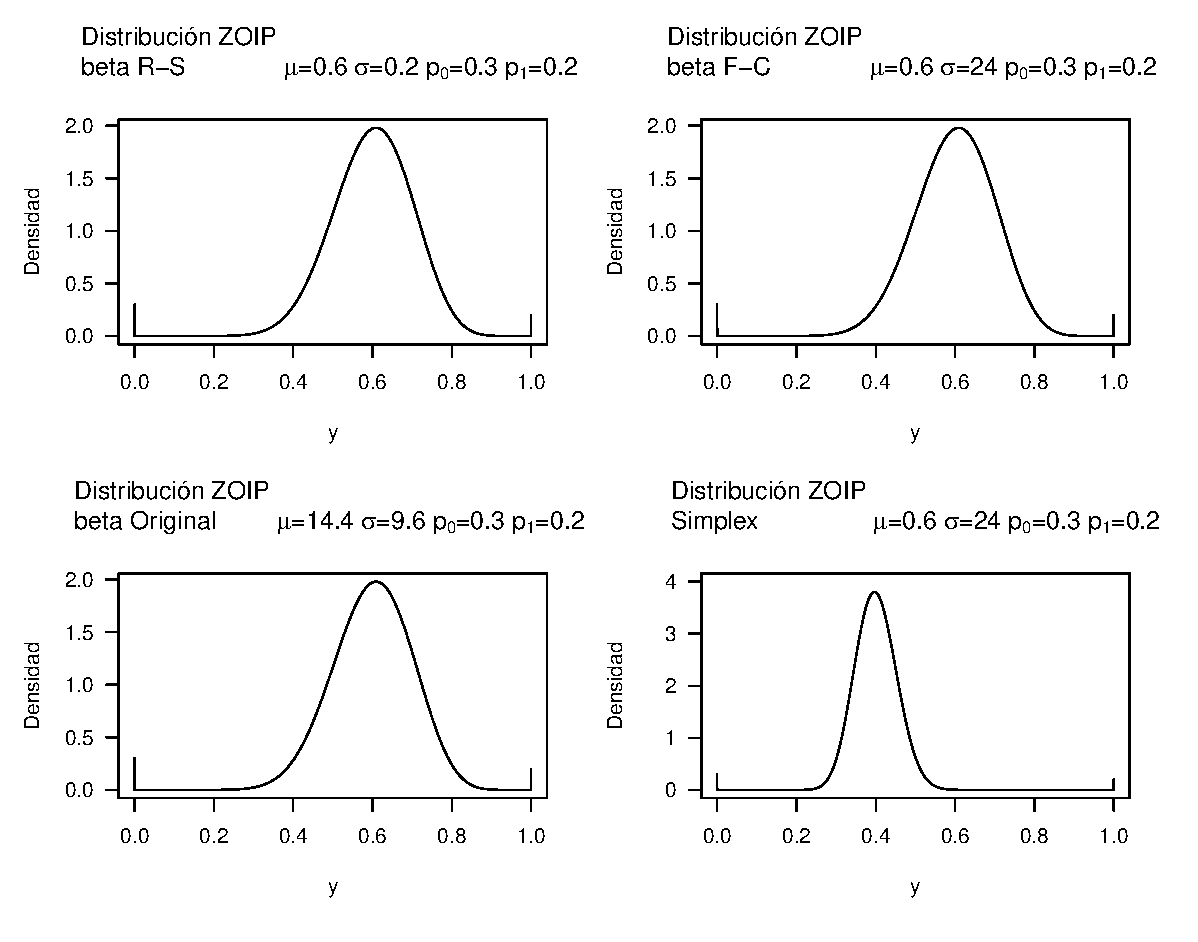
\includegraphics[scale=0.6]{Dist_ZOIP.eps}
		\caption{Densidades para la distribuci\'{o}n ZOIP para algunos valores de los par\'{a}metros, donde R-S se refiere a Rigby \& Stasinopoulos (2005) y F-C es Ferrari \& Cribari-Neto (2004).}
		\label{Dist_ZOIP}
	\end{center}
\end{figure}

%%%%%%%%%%%%%%%%%%%%%%%%%%%%%%%%%%%%%%%%%%%%%%%%%%%%%%%%%%%%%%%%%%%%%%%%%%%%%%%%%%%%%%%%%%%%%%%%%%%%%%%%%%%%%%%%%%%%%%%%%%%%%%%%%%%%%%%%%%%%%%%%%%%%%%%%%%%%%%%%%%
\section{Inferencia estad\'{\i}stica}

Para estimar los par\'{a}metros de la distribuci\'{o}n ZOIP se usa el m\'{e}todo de m\'{a}xima verosimilitud. La funci\'{o}n de verosimilitud para $\boldsymbol{\theta}=(\mu, \sigma, p_0, p_1)^{\top}$, basado en una muestra de $\boldsymbol{y}_i$ observaciones independientes, es de la forma:

\begin{equation}
L(\boldsymbol{\theta})=\prod_{i=1}^{n}g(\mathbf{y}_i;\mu, \sigma, p_0, p_1) 
\label{F_likel}
\end{equation}

%\[
%\ell(\boldsymbol{\theta})=\sum_{i=1}^{n}{\ell_i(\boldsymbol{\theta}) }
%\]

%donde para el caso de ZOIP-Beta original $\mu=p$, $\sigma=q$; si la distribuci\'{o}n ZOIP-Beta fuese con parametrizaci\'{o}n de \cite{Ferrari2} el \'{u}nico par\'{a}metro que cambiar\'{\i}a es $\sigma=\phi$, el resto de los par\'{a}metros no tendr\'{a}n modificaciones seg\'{u}n su parametrizaci\'{o}n o distribuci\'{o}n.\\

Para encontrar los estimadores de m\'{a}xima verosimilitud (MLE) de la distribuci\'{o}n ZOIP, se consideraran 2 casos:

\begin{enumerate}
	\item \textbf{ZOIP-beta original}\\
	Considera la parametrizaci\'{o}n de la distribuci\'{o}n beta original  y la ecuaci\'{o}n definida en \eqref{F_likel} se tiene que:
	\[
	\boldsymbol{\theta}=(p,q,p_0,p_1)^{\top}
	\]
	\[
	L(\boldsymbol{\theta})=\prod_{i=1}^{n}g(\boldsymbol{\theta}|y_i)=L_1(p_0)\cdot L_2(p_1) \cdot L_3(p,q)
	\]
	\\
Note que la funci\'{o}n de verosimilitud es factorizada en tres t\'{e}rminos, dos de ellos del componente discreto y uno compuesto por $p$ y $q$ del componente continuo, por tanto los par\'{a}metros son separables \citep{Pace1}, as\'{\i} la m\'{a}xima verosimilitud puede ser tratada por separado.\\
\[
L_1(p_0)=\prod_{i=1}^{n}p_0^{S_0(y_i)}(1-p_0)^{1-S_0(y_i)}=p_0^{\sum_{i=1}^{n}{S_0(y_i)}}(1-p_0)^{n-\sum_{i=1}^{n}{S_0(y_i)}}
\]
\\
donde:
\begin{equation}
S_j(y_i)=
\begin{cases}
1 & \text{si}\ y_i=j\\
0 & \text{si}\ y_i\neq j\\
\end{cases}
\quad ; \quad j=1,2 \label{Sj}
\end{equation}

Ahora sacando logaritmo natural a la funci\'{o}n de verosimilitud.
\[
\ell_1(p_0)=\sum_{i=1}^{n}{S_0(y_i)log(p_0)}+(n-\sum_{i=1}^{n}{S_0(y_i)})log(1-p_0)
\]	
\[
\frac{\delta \ell_1(p_0)}{\delta p_0}=\frac{\sum_{i=1}^{n}{S_0(y_i)}}{p_0}-\frac{n-\sum_{i=1}^{n}{S_0(y_i)}}{1-p_0}=\sum_{i=1}^{n}{S_0(y_i)}-p_0n=0
\]
\[
\hat{p_0}=\frac{1}{n}\sum_{i=1}^{n}{S_0(y_i)}
\]
\[
\therefore \hat{p_1}=\frac{1}{n}\sum_{i=1}^{n}{S_1(y_i)}
\]
\\
Ahora se halla MLE para los par\'{a}metros del componente continuo de la funci\'{o}n.

\[
\ell_3(p,q)=\sum_{i=1:y_i \in (0,1)}^{n}{log(f(p,q|y_i))}=n log(\Gamma(p+q))-n log(\Gamma(p))-n log(\Gamma(q))
\]
\[
+(p-1)\sum_{i=1:y_i \in (0,1)}^{n}{log(y_i)}+(q-1)\sum_{i=1:y_i \in (0,1)}^{n}{log(1-y_i)}
\]
\\
entonces
\[
\frac{\delta \ell_3(p,q)}{\delta p}=\sum_{i=1:y_i \in (0,1)}^{n}{log(y_i)}+\frac{n \cdot \delta log(\Gamma(p+q))}{\delta p}- \frac{n \cdot \delta log(\Gamma(p))}{\delta p}-\frac{n\cdot \delta log(\Gamma(q))}{\delta p}=0
\]
\[
\frac{\delta \ell_3(p,q)}{\delta q}=\sum_{i=1:y_i \in (0,1)}^{n}{log(1-y_i)}+\frac{n \cdot \delta log(\Gamma(p+q))}{\delta q}- \frac{n \cdot \delta log(\Gamma(p))}{\delta q}-\frac{n\cdot \delta log(\Gamma(q))}{\delta q}=0
\]

\[
\frac{\delta \ell_3(p,q)}{\delta p}=\sum_{i=1:y_i \in (0,1)}^{n}{log(y_i)}-n(-\psi(p+q)+\psi(p))=0
\]
\[
\frac{\delta \ell_3(p,q)}{\delta q}=\sum_{i=1:y_i \in (0,1)}^{n}{log(1-y_i)}-n(-\psi(p+q)+\psi(q))=0
\]
\\
donde $\psi(\cdot)={\Gamma^{'}{(\cdot)}}/{\Gamma(\cdot)}$
\\
Este sistema de ecuaciones no tiene una soluci\'{o}n de forma cerrada, por lo que para encontrar los MLE de $p$ y $q$ es necesario utilizar algoritmos iterativos, por ejemplo el m\'{e}todo de Newton Raphson, m\'{\i}nimos cuadrados ponderados y en el paquete \pkg{ZOIP} se utiliza optimizadores a la funci\'{o}n de verosimilitud mediante la funci\'{o}n \code{nlminb} de \proglang{R}, sin embargo se puede garantizar que los puntos cr\'{\i}ticos encontrados ser\'{a}n m\'{a}ximos de la funci\'{o}n de verosimilitud, ya que si hallamos la segunda derivada de la funci\'{o}n se tiene que:
\[
\frac{\delta^2 \ell_3(p,q)}{\delta p^2}=-n(\psi^{'}(p)-\psi^{'}(p+q))<0
\]
\[
\frac{\delta^2 \ell_3(p,q)}{\delta q^2}=-n(\psi^{'}(q)-\psi^{'}(p+q))<0
\]
\\
debido que la varianza de la transformaci\'{o}n logar\'{\i}tmica de la variable es:
\[
var(log(y))=E[log^2(y)]-(E[log(y)])^2=\psi^{'}(p)-\psi^{'}(p+q)>0
\]
\[
var(log(1-y))=E[log^2(1-y)]-(E[log(1-y)])^2=\psi^{'}(q)-\psi^{'}(p+q)>0
\]
\\
ver m\'{a}s en \cite{Owen1}.\\

Para encontrar las estimaciones de los par\'{a}metros de beta en parametrizaciones de \cite{Ferrari2} y \cite{Stasinopoulos2}, basta con encontrar los estimadores MLE anteriores de la parametrizaci\'{o}n original y utilizar las ecuaciones definidas en \eqref{FC_Origin1}, \eqref{FC_Origin2} para el caso de \cite{Ferrari2} y \eqref{RS_Origin1}, \eqref{RS_Origin2} para el caso de \cite{Stasinopoulos2}.

\item \textbf{ZOIP-simplex}\\

Para este caso lo \'{u}nico que var\'{\i}a con respecto al anterior es la estimaci\'{o}n en el componente continuo.

\[
L_3(\mu,\sigma)=\prod_{i=1:y_i \in (0,1)}^{n}\left[{2\pi \sigma^{2}[y_i(1-y_i)]^{3}}\right]^{-1/2}exp\left(-\frac{1}{2\sigma^2}d(y_i;\mu)\right)
\]
\\
donde $d(y_i ;\mu)=\frac{y_i(1-y_i)\mu^2(1-\mu)^2}{(y_i-\mu)^2}$
\[
\ell_3(\mu,\sigma)=-\frac{n}{2}log(2\pi)-\frac{n}{2}log(\sigma^2)-\frac{3}{2}\sum_{i=1:y_i \in (0,1)}^{n}{log(y_i(1-y_i))}-\sum_{i=1:y_i \in (0,1)}^{n}{\frac{1}{2\sigma^2}d(y_i;\mu)}
\]

\[
\frac{\delta \ell_3(\mu,\sigma)}{\delta \sigma}=-\frac{n}{\sigma}+\frac{1}{\sigma^3}\sum_{i=1:y_i \in (0,1)}^{n}{d(y_i;\mu)}=\sigma(-n\sigma^2+\sum_{i=1:y_i \in (0,1)}^{n}{d(y_i;\mu))}=0
\]
\\
no es admisible que $\sigma=0$ entonces:
\[
-n\sigma^2+\sum_{i=1:y_i \in (0,1)}^{n}{d(y_i;\mu)}=0
\]
\[
\therefore \hat{\sigma^2}=\frac{1}{n}\sum_{i=1:y_i \in (0,1)}^{n}{d(y_i;\mu)}
\]
\\
El estimador MLE de $\sigma^2$ depende del valor estimado en $\mu$, entonces:
\[
\frac{\delta \ell_3(\mu,\sigma)}{\delta \sigma}=-\frac{1}{2\sigma^2}\sum_{i=1:y_i \in (0,1)}^{n}{\frac{\delta d(y_i;\mu)}{\delta\mu}}=0
\]

\begin{multline*}
\frac{\delta d(y_i;\mu)}{\delta\mu}=\sum_{i=1:y_i \in (0,1)}^{n}\frac{y_i(1-y_i)\mu^2(1-\mu)^2}{2(y_i-\mu)^3}\\
+\frac{2y_i(1-y_i)\mu(1-\mu)^2-2y_i(1-y_i)\mu^2(1-\mu)}{(y_i-\mu)^2}=0
\end{multline*}

No tiene una soluci\'{o}n cerrada anal\'{\i}ticamente, entonces se deben utilizar algoritmos iterativos tal como Newton Raphson o m\'{\i}nimos cuadrados ponderados, en el paquete \pkg{ZOIP} se utiliza optimizadores para la funci\'{o}n de verosimilitud mediante la funci\'{o}n \code{nlminb} de \proglang{R}, para encontrar puntos cr\'{\i}ticos donde ${\delta d(y_i;\mu)}/{\delta\mu}=0$.

\end{enumerate}

%%%%%%%%%%%%%%%%%%%%%%%%%%%%%%%%%%%%%%%%%%%%%%%%%%%%%%%%%%%%%%%%%%%%%%%%%%%%%%%%%%%%%%%%%%%%%%%%%%%%%%%%%%%%%%%%%%%%%%%%%%%%%%%%%%%%%%%%%%%%%%%%%%%%%%%%%%%%%%%%%%


\section{Distribuci\'{o}n ZOIP en el paquete \pkg{ZOIP}}

En esta secci\'{o}n se presenta el paquete \pkg{ZOIP} de \proglang{R} alojado en \verb|GitHub| y creado por los autores para analizar datos proporcionales inflados con ceros y/o unos y ajustar una distribuci\'{o}n ZOIP.

\subsection{Instalaci\'{o}n}

Para acceder a la \'{u}ltima versi\'{o}n del paquete \pkg{ZOIP}, se encuentra ubicada en \verb|GitHub|, el cual es un alojamiento de repositorios Git, para obtener dicha versi\'{o}n es necesario ejecutar el siguiente c\'{o}digo que instala el paquete \pkg{devtools}, que es necesario para descargar el paquete \pkg{ZOIP} y otros paquetes complementarios, para el correcto funcionamiento del paquete.

\begin{verbatim}
if (!require('devtools')) install.packages('devtools')
if (!require('rmutil')) install.packages('rmutil')
if (!require('boot')) install.packages('boot')
if (!require('numDeriv')) install.packages('numDeriv')
if (!require('GHQp')) install.packages('GHQp')
devtools::install_github('jucdiaz/ZOIP', force=TRUE)
library(ZOIP)  # Carga el paquete
\end{verbatim}

\subsection{Funciones sobre distribuci\'{o}n ZOIP}

En el paquete \pkg{ZOIP} existen cuatro funciones llamadas \code{dZOIP}, \code{pZOIP}, \code{qZOIP} y \code{rZOIP} el cual corresponden a las funciones de densidad de probabilidad, la funci\'{o}n de distribuci\'{o}n acumulada, la funci\'{o}n cuantil y la funci\'{o}n generadora de n\'{u}meros aleatorios de la distribuci\'{o}n ZOIP, respectivamente; en el siguiente c\'{o}digo se observa como se halla la densidad de probabilidad en el punto $0.5$ de una distribuci\'{o}n ZOIP-beta con parametrizaci\'{o}n \cite{Stasinopoulos2} descrita como $\text{ZOIP}(\mu=0.2, \, \sigma=0.5, \, p_0=0.2, \, p_1=0.2)$\\

\begin{verbatim}
dZOIP(x=0.5, mu=0.2, sigma=0.5, p0=0.2, p1=0.2, family='R-S')
##[1] 0.3243543
\end{verbatim}

Adem\'{a}s se halla la probabilidad acumulada hasta el punto $0.5$ de una distribuci\'{o}n OIP-beta con parametrizaci\'{o}n \cite{Ferrari2} dada por $\text{ZOIP}(\mu=0.2, \, \sigma=3, \, p_0=0, \, p_1=0.2)$\\

\begin{verbatim}
pZOIP(q=0.5, mu=0.2, sigma=3, p0=0, p1=0.2, family='F-C')
##[1] 0.7181223
\end{verbatim}

Se calcula el percentil en el punto $0.7$ de una distribuci\'{o}n ZIP-beta original dada por $\text{ZOIP}(\mu=0.6, \, \sigma=2.4, \, p_0=0.2, \, p_1=0)$\\

\begin{verbatim}
qZOIP(p=0.7, mu=0.6, sigma=2.4, p0=0.2, p1=0, family='Original')
##[1] 0.2061418
\end{verbatim}

Por \'{u}ltimo se generaron 8 valores aleatorios de una distribuci\'{o}n ZOIP-simplex descrita como $\text{ZOIP}(\mu=0.6, \, \sigma=3, \, p_0=0.2, \, p_1=0.2)$. La funci\'{o}n \code{set.seed} sirve para garantizar la repetici\'{o}n de los valores aleatorios generados en el ejemplo.\\

\begin{verbatim}
set.seed(12345)
rZOIP(n=8, mu=0.2, sigma=3, p0=0.2, p1=0.2, family='Simplex')
##[1] 0.3185479 1.0000000 0.3765073 1.0000000 0.1626598
##[6] 0.0000000 0.1138673 0.1840670
\end{verbatim}

\subsection{Funci\'{o}n RM.ZOIP}

La funci\'{o}n \code{RM.ZOIP} estima los par\'{a}metros de una distribuci\'{o}n ZOIP, v\'{\i}a m\'{a}xima verosimilitud utilizando el optimizador deseado (\code{nlminb}, \code{optim}). La estructura de la funci\'{o}n \code{RM.ZOIP} es la siguiente:

\begin{verbatim}
RM.ZOIP(
  formula.mu,
  formula.sigma = ~ 1,
  formula.p0 = ~ 1,
  formula.p1 = ~ 1,
  data,
  link = c('identity', 'identity', 'identity', 'identity'),
  family = 'R-S',
	optimizer='nlminb'
)
\end{verbatim}

Los argumentos de la funci\'{o}n \code{RM.ZOIP} son:

\begin{itemize}[noitemsep, nolistsep]

\item \code{formula.mu}: Formula que define la funci\'{o}n de regresi\'{o}n para el par\'{a}metro $\mu$, Para ajustar una distibuci\'{o}n ZOIP debe tomar el valor de \code{y $\sim$ 1}, donde y es la variable a ajustar.
\item \code{formula.sigma}: Formula que define la funci\'{o}n de regresi\'{o}n para el par\'{a}metro $\sigma$, Para ajustar una distibuci\'{o}n ZOIP debe tomar el valor de \code{$\sim$ 1}.
\item \code{formula.p0}: Formula que define la funci\'{o}n de regresi\'{o}n para el par\'{a}metro $p_0$, Para ajustar una distibuci\'{o}n ZOIP debe tomar el valor de \code{$\sim $1}.
\item \code{formula.p1}: Formula que define la funci\'{o}n de regresi\'{o}n para el par\'{a}metro $p_1$,Para ajustar una distibuci\'{o}n ZOIP debe tomar el valor de \code{$\sim $1}.
\item \code{data}: es el conjunto de datos en formato \code{data.frame} donde debe contener los datos de la variable a ajustar y el nombre debe ser la tal cual como est\'{a} en las f\'{o}rmula para el par\'{a}metro $\mu$.
\item \code{family}: Elecci\'{o}n de la distribuci\'{o}n ZOIP deseada para ajustar, si toma el valor de \code{`R-S'} se utilizar\'{a} la distribuci\'{o}n ZOIP-beta con parametrizaci\'{o}n  \cite{Stasinopoulos2}, si toma el valor de \code{`F-C'} se utilizar\'{a} la distribuci\'{o}n ZOIP-beta parametrizaci\'{o}n \cite{Ferrari2}, el valor de \code{`Original'} se utilizar\'{a} la distribuci\'{o}n ZOIP-beta con parametrizaci\'{o}n original, \code{`Simplex'} Utilizar\'{a} la distribuci\'{o}n ZOIP-simplex.
\item \code{link}: Es un vector con las funciones enlace adecuadas para cada par\'{a}metro a estimar de acuerdo a las opciones escogidas en los par\'{a}metros de familia y formula. Para ajustar una distribuci i\'{o}n ZOIP se debe utilizar como funci\'{o}n enlace la opci\'{o}n \code{identity} en sus cuatro par\'{a}metros, independientemente de la distribuci i\'{o}n ZOIP escogida, en familia. Por defecto \code{link=c(`identity',`identity',`identity',`identity')}.
\item \code{optimizer}: Elecci\'{o}n del optimizador, utilizado para encontrar la convergencia de la m\'{a}xima verosimilitud. se puede elegir el valor de \code{`nlminb'} o \code{`optim'}. Por defecto \code{`nlminb'}
\end{itemize}

En el siguiente ejemplo se mostrara el ajuste de una distribuci\'{o}n ZOIP, para ello mostraremos la salida de la funci\'{o}n \code{RM.ZOIP} de $1000$ observaciones simuladas para la distribuci\'{o}n ZOIP-beta parametrizaci\'{o}n \cite{Stasinopoulos2}.\\

\begin{verbatim}
yi <- as.data.frame(rZOIP(n=1000, mu=0.6, sigma=0.2,
                          p0=0.03, p1=0.05, family='R-S'))
mod <- RM.ZOIP(formula.mu=yi ~ 1, formula.sigma= ~ 1, 
               formula.p0= ~ 1, formula.p1= ~ 1, data=yi,
               family='R-S')
summary(mod)
\end{verbatim}

\begin{verbatim}
---------------------------------------------------------------
Fixed effects for identity(mu)
---------------------------------------------------------------
             Estimate Std. Error z value  Pr(>|z|)    
(intercept) 0.6066914  0.0031636  191.78 < 2.2e-16 ***
---
Signif. codes:  0 *** 0.001 ** 0.01 * 0.05 . 0.1   1
---------------------------------------------------------------
Fixed effects for identity(sigma)
---------------------------------------------------------------
            Estimate Std. Error z value  Pr(>|z|)    
(intercept) 0.196643   0.004322  45.498 < 2.2e-16 ***
---
Signif. codes:  0 *** 0.001 ** 0.01 * 0.05 . 0.1   1
---------------------------------------------------------------
Fixed effects for identity(p0)
---------------------------------------------------------------
             Estimate Std. Error z value Pr(>|z|)    
(intercept) 0.0339992  0.0057308  5.9327 2.98e-09 ***
---
Signif. codes:  0 *** 0.001 ** 0.01 * 0.05 . 0.1   1
---------------------------------------------------------------
Fixed effects for identity(p1)
---------------------------------------------------------------
             Estimate Std. Error z value  Pr(>|z|)    
(intercept) 0.0450005  0.0065556  6.8644 6.675e-12 ***
---
Signif. codes:  0 *** 0.001 ** 0.01 * 0.05 . 0.1   1
---------------------------------------------------------------
---------------------------------------------------------------
\end{verbatim}

En el resultado anterior se obtienen los valores de $\hat{\mu}=0.6066914$, $\hat{\sigma}=0.196643$, $\hat{p_0}=0.0339992$ y $\hat{p_1}=0.0450005$, que son a los par\'{a}metros con los que se simulo $y_i$. Adem\'{a}s cabe resaltar que en la funci\'{o}n \code{RM.ZOIP} para ajustar distribuciones de probabilidad no es necesario colocar funciones de enlace ni espacio de busqueda de los par\'{a}metros, ya que estos son introducidas autom\'{a}ticamente de acuerdo a el valor tomado en \code{family}.

%%%%%%%%%%%%%%%%%%%%%%%%%%%%%%%%%%%%%%%%%%%%%%%%%%%%%%%%%%%%%%%%%%%%%%%%%%%%%%%%%%%%%%%%%%%%%%%%%%%%%%%%%%%%%%%%%%%%%%%%%%%%%%%%%%%%%%%%%%%%%%%%%%%%%%%%%%%%%%%%%%

\section{Aplicaci\'{o}n}
En esta secci\'{o}n se muestran varios resultados sobre el ajuste de una distribuci\'{o}n ZOIP, primero se realiz\'{o} un estudio de simulaci\'{o}n para observar la convergencia de la estimaci\'{o}n de los par\'{a}metros de la distribuci\'{o}n, y en segunda instancia se ajust\'{o} una distribuci\'{o}n ZOIP a datos reales sobre la utilizaci\'{o}n de una tarjeta de cr\'{e}dito de una entidad financiera.

\subsection{Datos simulados}
En este estudio de simulaci\'{o}n se analizan diferentes aspectos de la capacidad de estimaci\'{o}n que tiene el m\'{e}todo de m\'{a}xima verosimilitud sobre los par\'{a}metros de la distribuci\'{o}n ZOIP. Se generaron muestras de una distribuci\'{o}n ZOIP bajo las diferentes distribuciones y par\'{a}metrizaciones con tama\~{n}os de muestra n de: 5, 10, 15 y as\'{\i} sucesivamente hasta 500, y se realizaron 1000 r\'{e}plicas para cada tama\~{n}o de muestra, posteriormente se calcul\'{o} la mediana de cada una de las estimaciones de los par\'{a}metros, y as\'{\i} poder analizar la capacidad de convergencia de las metodolog\'{\i}as implementadas en la distribuci\'{o}n ZOIP y en el paquete \pkg{ZOIP}.\\

En el primer escenario del estudio de simulaci\'{o}n se generaron los datos de una distribuci\'{o}n ZOIP-beta$(\mu=0.6 ,\sigma=0.2 , p_0=0.03 , p_1= 0.05)$ para el caso de la parametrizaci\'{o}n de \cite{Stasinopoulos2}, ZOIP-beta$(\mu=0.6 , \sigma=24 , p_0=0.03 , p_1= 0.05)$ para el caso de la parametrizaci\'{o}n de \cite{Ferrari2}, ZOIP-beta$(\mu=14.4 , \sigma=9.6 , p_0=0.03 , p_1= 0.05)$ en la parametrizaci\'{o}n original, cabe aclarar que las tres parametrizaciones anteriores generan exactamente la misma distribuci\'{o}n, esto gracias a las ecuaciones definidas en \eqref{FC_Origin1}, \eqref{FC_Origin2}, \eqref{RS_Origin1} y \eqref{RS_Origin2}, de igual manera se gener\'{o} la misma cantidad de datos simulados para la distribuci\'{o}n ZOIP-simplex$(\mu=0.4 , \sigma=0.2 , p_0=0.03 , p_1= 0.05)$.\\


\begin{figure}
	\begin{center}
		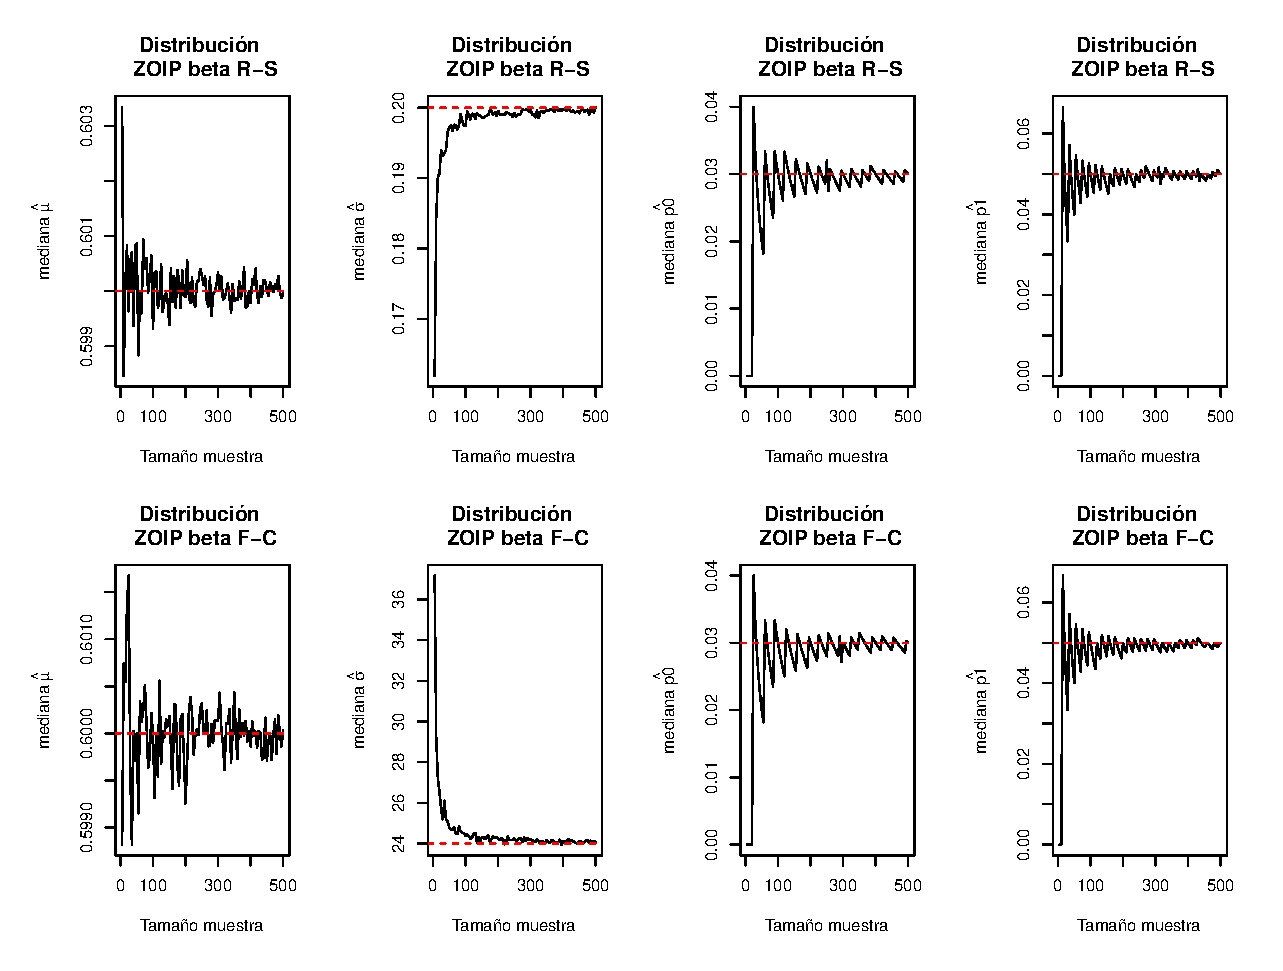
\includegraphics[scale=0.55]{Simulacion_RS_FC.eps}
		\quad
		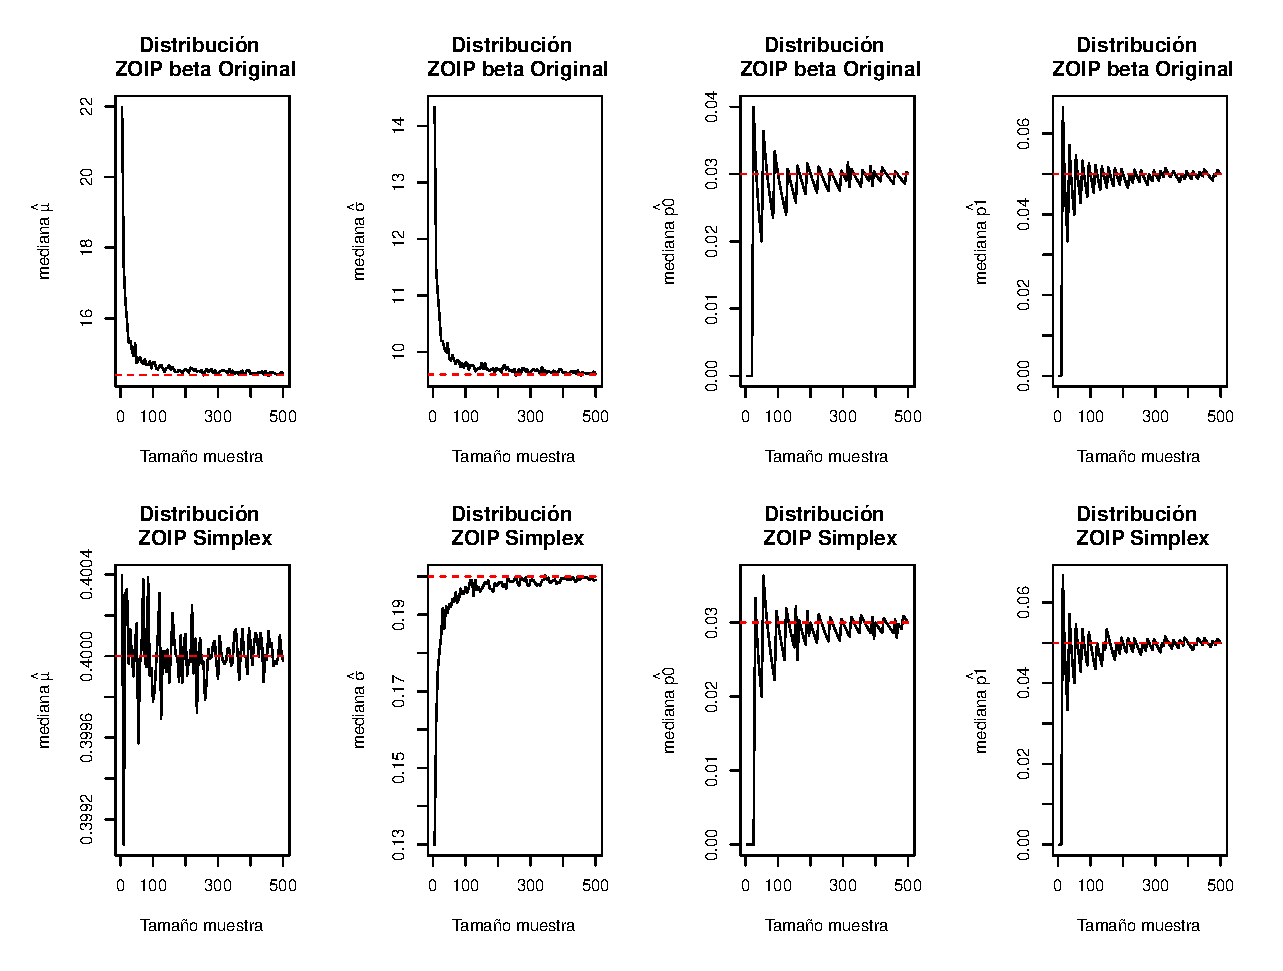
\includegraphics[scale=0.55]{Simulacion_Ori_Sim.eps}	
		\caption{Mediana de los par\'{a}metros estimados en el escenario 1 para distintas parametrizaciones y valores de $n$, las l\'{\i}neas rojas representan el verdadero valor del par\'{a}metro.}
		\label{Simu_1}
	\end{center}
\end{figure}

En la Figura \ref{Simu_1} se presentan las medianas de la estimaci\'{o}n de los par\'{a}metros para cada tama\~{n}o de muestra, de esta figura se observa que independientemente de la distribuci\'{o}n y pa\-ra\-me\-tri\-za\-ci\-\'{o}n escogida en la distribuci\'{o}n ZOIP, todos las estimaciones convergen al valor verdadero del par\'{a}metro a medida que aumenta el tama\~{n}o de muestra n, de la Figura \ref{Simu_1} se nota que las estimaciones de $\sigma$ cuando son par\'{a}metros con significado de dispersi\'{o}n como es en la distribuci\'{o}n beta con parametrizaci\'{o}n \cite{Stasinopoulos2} y en la distribuci\'{o}n simplex, tienden a dar valores subestimados, por otra parte, en las distribuciones que $\sigma$ tiene significado de forma y precisi\'{o}n tienden a dar valores sobrestimados. Se observa que las estimaciones de los par\'{a}metros de inflaci\'{o}n a pesar de que son peque\~{n}as dan resultados muy satisfactorios y casi sin variaci\'{o}n en su forma de estimaci\'{o}n de distribuci\'{o}n a distribuci\'{o}n.\\

Como medida global del proceso de estimaci\'{o}n se eligi\'{o} el MAPE (Error porcentual absoluto medio. $(\sum_{i=1}^{n}{|y_i-\hat{y_i}/y_i}|)/n$) debido a los cambios de escala entre los diferentes par\'{a}metros de las diferentes distribuciones y parametrizaciones. Esta media se realiz\'{o} como un promedio de los MAPES generados por cada uno de los par\'{a}metros de la distribuci\'{o}n ZOIP en cada tama\~{n}o de muestra. En la Figura \ref{Mapes}a se presenta el MAPE para las diferentes distribuciones y parametrizaciones estimadas, se observa como a medida que el tama\~{n}o de muestra aumenta, el MAPE va decreciendo r\'{a}pidamente, aunque des\-pu\'{e}s de un tama\~{n}o de muestra de 200, el MAPE decrece de una manera m\'{a}s lenta, adem\'{a}s los errores de estimaci\'{o}n son muy parecidos entre los cuatro casos de simulaci\'{o}n, la estimaci\'{o}n sobre los par\'{a}metros de la distribuci\'{o}n ZOIP-simplex tiene un error un poco m\'{a}s grande, pero no es significativo sobre los dem\'{a}s casos.\\
 
En el segundo escenario de simulaci\'{o}n se gener\'{o} el mismo ejercicio de simulaci\'{o}n anterior sobre las mismas distribuciones y parametrizaciones, solo que los valores de $p_0$ y $p_1$ cambian por $0.3$ y $0.2$, respectivamente. Dando as\'{\i} que el 50\% de los datos se vean contaminados por ceros y unos, esto para ver si de alguna forma afecta el aumento de la presencia de ceros y unos sobre las estimaciones de los par\'{a}metros de la parte continua de la distribuci\'{o}n ZOIP.

\begin{figure}
	\begin{center}
		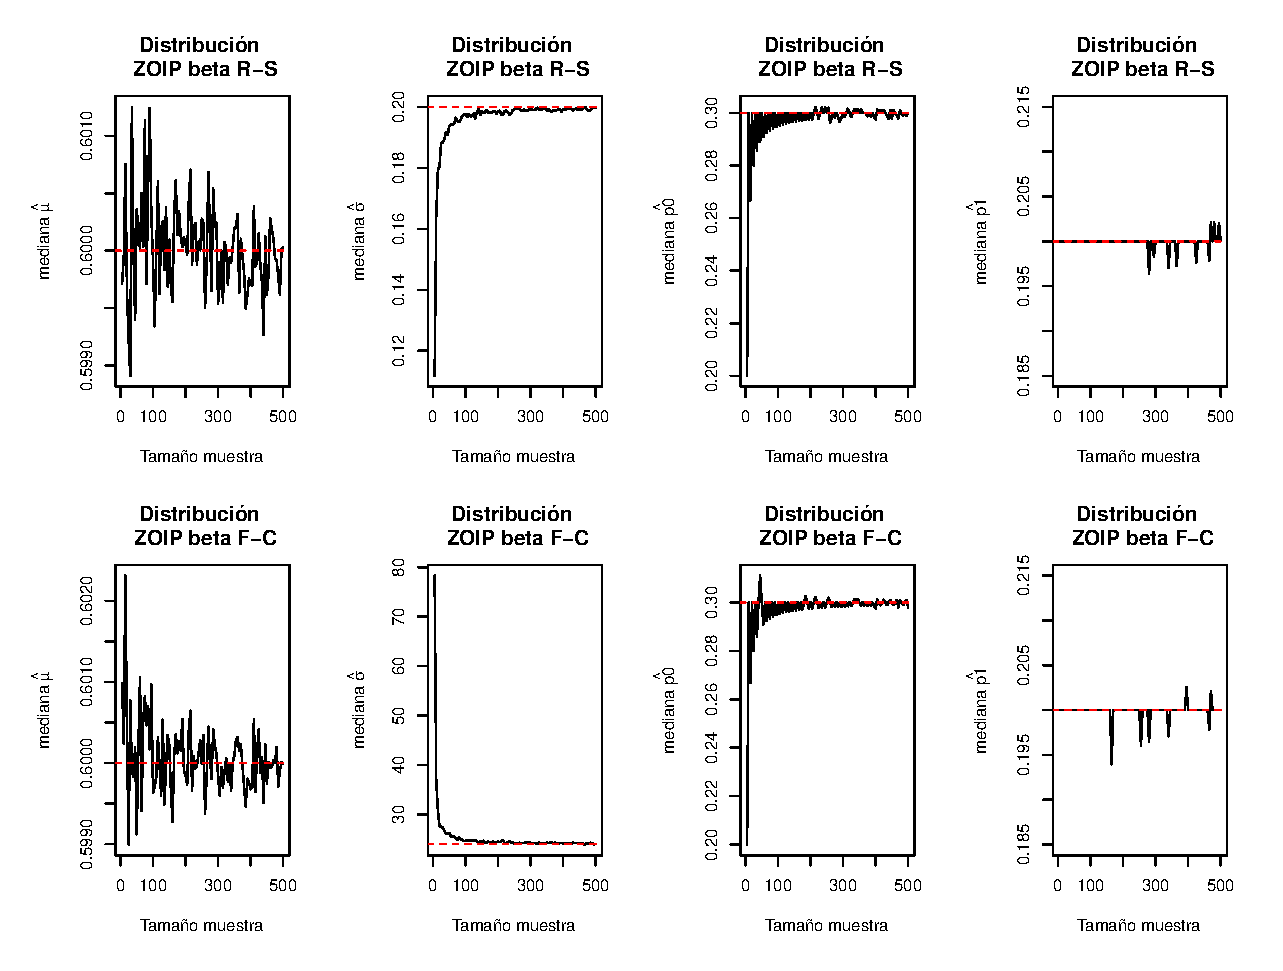
\includegraphics[scale=0.55]{Simulacion_RS_FC_Infla.eps}
		\quad
		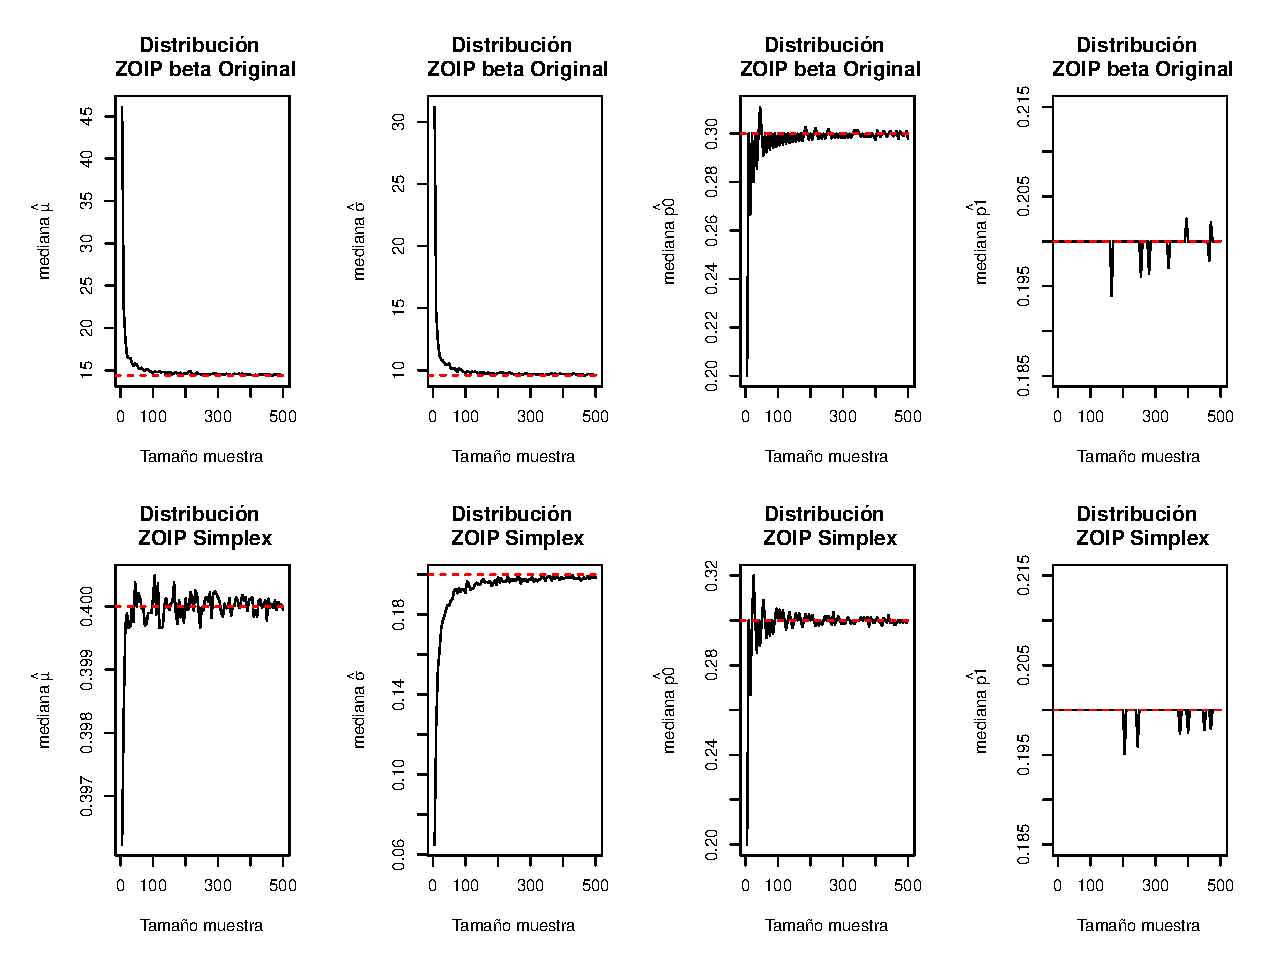
\includegraphics[scale=0.55]{Simulacion_Ori_Sim_Infla.eps}	
		\caption{Simulaci\'{o}n de distribuci\'{o}n ZOIP para distintas par\'{a}metrizaciones con par\'{a}metros de inflaci\'{o}n grandes, distribuciones y valores de $n$.}
		\label{Simu_2}
	\end{center}
\end{figure}

En la Figura \ref{Simu_2} se presentan las estimaciones de los par\'{a}metros de la simulaci\'{o}n con inflaciones al 50\% para diferentes tama\~{n}os de muestras, en general se observa que no se ven cambios muy significativos sobre la Figura \ref{Simu_1} en los par\'{a}metros de $\mu$ y $\sigma$, sin embargo, en la estimaci\'{o}n de $p_0$ se tienden a dar valores subestimados con relaci\'{o}n al estudio de simulaci\'{o}n anterior y con el par\'{a}metro $p_1$ aunque las estimaciones son muy acertadas sobre el valor real desde tama\~{n}os de muestra peque\~{n}os, en algunas ocasiones se producen peque\~{n}as perturbaciones no muy alejados del valor real.


\begin{figure}
	\begin{center}
		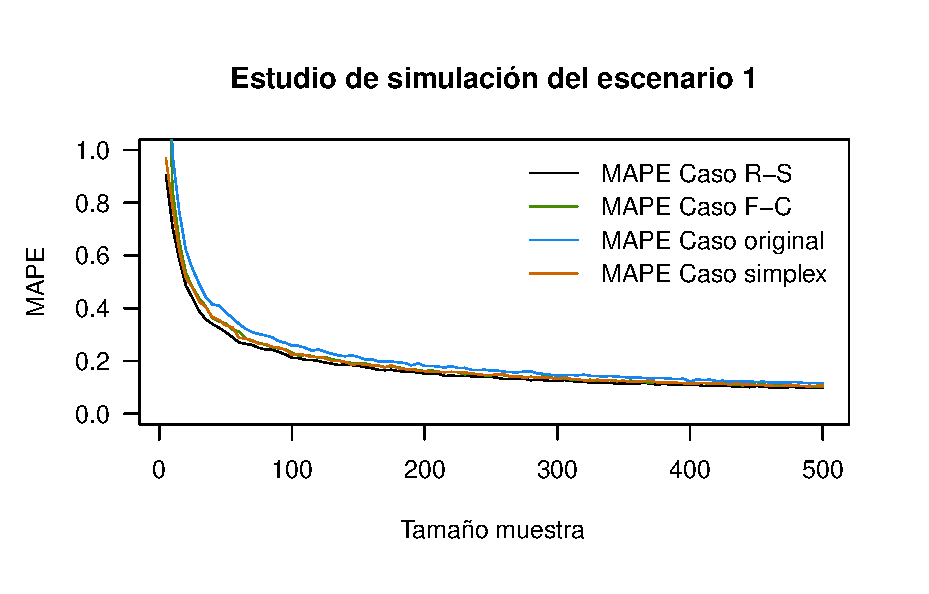
\includegraphics[scale=0.45]{Mape_gnrl.eps}	
		\quad
		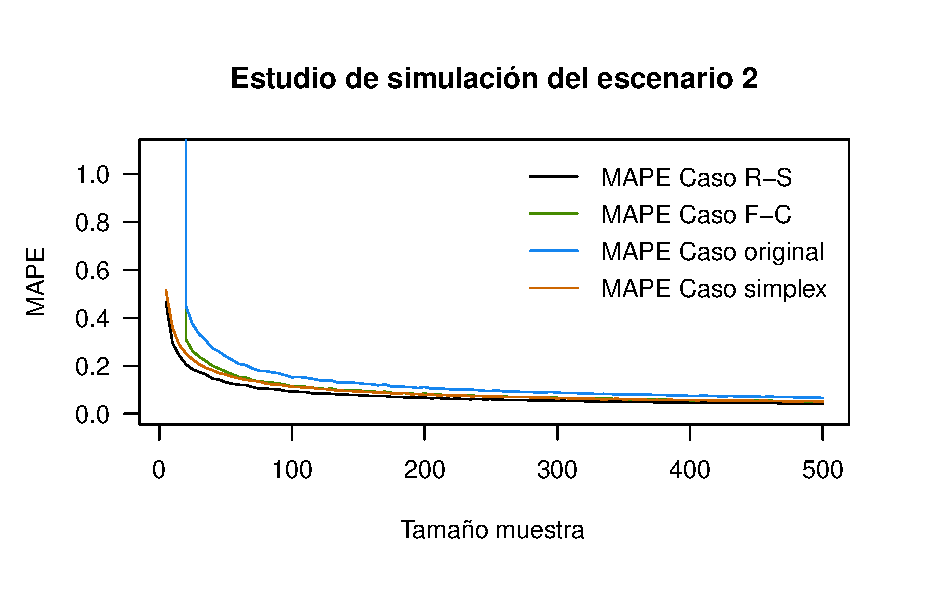
\includegraphics[scale=0.45]{Mape_gnrl_infla.eps}
		\caption{Mape (Error porcentual absoluto medio) para los dos escenarios de simulaci\'{o}n y para distintas parametrizaciones y valores de $n$.}
		\label{Mapes}
	\end{center}
\end{figure}

\begin{table}[!hbt]
{\scriptsize
\begin{center}
\begin{tabular}{|c|l|cc|}\hline
 Par\'{a}metro & Caso & MAPE escenario 1 \% &  MAPE escenario 2 \% \\ \hline

\multirow{4}{*}{$\mu$}&Caso R-S &0.61 & 0.86	\\
& Caso F-C & 0.50	& 0.85	\\
& Caso original &0.53 & 0.70	 \\
& Caso simplex 	&0.47 & 0.63	\\ \hline

\multirow{4}{*}{$\sigma$} &Caso R-S &2.53 & 3.40\\
& Caso F-C 	&5.10 & 6.90\\
& Caso original &5.30 & 6.98\\
& Caso simplex 	&5.30  &7.37 \\\hline

\multirow{4}{*}{$p_0$} &Caso R-S &20.5  & 5.36	\\
& Caso F-C &19.7  & 5.42	\\
& Caso original &19.8 & 5.43	\\
& Caso simplex 	&20.8 & 5.51\\ \hline

\multirow{4}{*}{$p_1$} &Caso R-S 	&15.2 & 7.28\\
& Caso F-C &16 & 7  \\
& Caso original &15.7	 & 7	\\
& Caso simplex &16.2 & 7.12	 \\ \hline
& Promedio & 10.57 & 5.26 \\ \hline
\end{tabular}
\caption{MAPE de las estimaciones para cada par\'{a}metro en diferentes parametrizaciones en los dos estudios de simulaci\'{o}n.}
\label{T_MAPES}
\end{center}
}
\end{table}

En la Figura \ref{Mapes}b se presenta el MAPE para el estudio de simulaci\'{o}n del escenario 2, se puede ver como se obtienen MAPES muy parecidos a los del estudio de simulaci\'{o}n del escenario 1, pero cabe resaltar como se comete menos error sobre la estimaci\'{o}n de los par\'{a}metros de la distribuci\'{o}n beta con parametrizaci\'{o}n \cite{Stasinopoulos2}. En la tabla \ref{T_MAPES} se presenta el MAPE para cada par\'{a}metro de cada parametrizaci\'{o}n para ambos estudios de simulaci\'{o}n, es claro ver como en general el estudio de simulaci\'{o}n del escenario 2 produce un MAPE menor que el del escenario 1, esto es causado por que en el escenario 1 de simulaci\'{o}n los errores de pron\'{o}stico son m\'{a}s grandes en los par\'{a}metros de inflaci\'{o}n que en el escenario 2. Por todo lo visto anteriormente se puede concluir que el crecimiento de los par\'{a}metros de inflaci\'{o}n no afecta de manera significativa la estimaci\'{o}n de los par\'{a}metros de la parte continua de la distribuci\'{o}n ZOIP, pero si en una mejor estimaci\'{o}n de los par\'{a}metros de inflaci\'{o}n.


\subsection{Datos reales}
En esta secci\'{o}n se presenta el ajuste de una distribuci\'{o}n ZOIP a datos reales sobre la utilizaci\'{o}n de una tarjeta de cr\'{e}dito en un banco, para una entidad financiera grande como un banco es de vital importancia conocer el comportamiento del porcentaje de utilizaci\'{o}n de sus tarjetas de cr\'{e}dito (tdc), se define a $y$ como el porcentaje de uso de una tdc, en la Figura \ref{hist_tdc} se presenta el histograma del porcentaje de utilizaci\'{o}n de las tdc y es claro notar que $y$ se encuentra entre cero y uno, pero adicional es muy com\'{u}n ver que las tdc no sean utilizadas ($y=0$) y tambi\'{e}n que las tdc sean utilizadas en la totalidad de su cupo asignado ($y=1$), por lo que se trata a $y$ como una variable aleatoria perteneciente a datos proporcionales inflados con ceros y unos. Se tiene un total de $9206$ tdc, que representan el porcentaje de utilizaci\'{o}n de las tdc para un trimestre del a\~{n}o 2014 del banco. Se quiere estudiar el ajuste de una distribuci\'{o}n ZOIP, para ello se utiliza el paquete en \proglang{R} llamado \pkg{ZOIP} mediante su funci\'{o}n \code{RM.ZOIP}.\\

\begin{figure}
	\begin{center}
		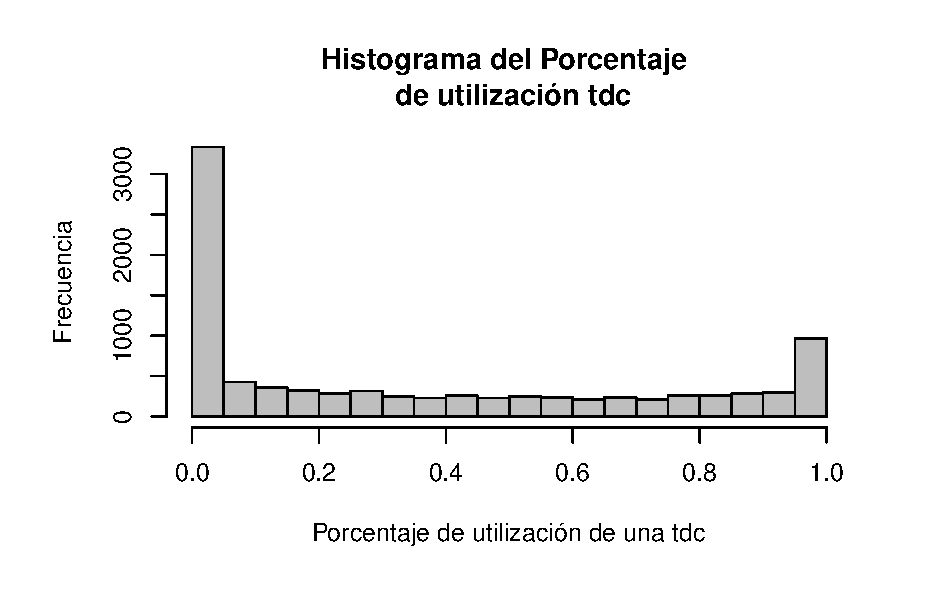
\includegraphics[scale=0.6]{Hist_tdc.eps}
		\caption{Histograma del porcentaje de utilizaci\'{o}n de las tdc en un banco.}
		\label{hist_tdc}
	\end{center}
\end{figure}

\begin{table}[!hbt]
{\scriptsize
\begin{center}
\begin{tabular}{|c|c|ccc|c|}\hline
Familia & Par\'{a}metro & Estimaci\'{o}n & Error est\'{a}ndar & Valor P & Log-Verosimilitud\\ \hline

\multirow{4}{*}{R-S} &$\mu$ &0.4040	&0.0037	&$<2.2e^{-16}$ &\multirow{4}{*}{5854.067}\\
& $\sigma$ & 0.6601	&0.0027	&$<2.2e^{-16}$& \\
& $p_0$ & 0.2219	&0.0043	&$<2.2e^{-16}$ &\\
& $p_1$ & 0.0695	&0.0027	&$<2.2e^{-16}$ &\\ \hline

\multirow{4}{*}{F-C} &$\mu$ & 0.4040	&0.0037	&$<2.2e^{-16}$ &\multirow{4}{*}{5854.067}\\
& $\sigma$ & 0.4040	&0.0037	&$<2.2e^{-16}$ &\\
& $p_0$ & 0.2219	&0.0043	&$<2.2e^{-16}$ &\\
& $p_1$ & 0.0695	&0.0027	&$<2.2e^{-16}$ &\\ \hline

\multirow{4}{*}{original} &$\mu$ & 0.5233	&0.0080	&$<2.2e^{-16}$&\multirow{4}{*}{5854.067} \\
& $\sigma$ & 0.7719	&0.0130	&$<2.2e^{-16}$& \\
& $p_0$ & 0.2219	&0.0043	&$<2.2e^{-16}$& \\
& $p_1$ & 0.0695	&0.0027	&$<2.2e^{-16}$& \\ \hline

\multirow{4}{*}{simplex} &$\mu$ & 0.5741	&0.0010	&$<2.2e^{-16}$ &\multirow{4}{*}{54425.63}\\
& $\sigma$ & 4885.4370	&18.2430	&$<2.2e^{-16}$ &\\
& $p_0$ & 0.1497	&0.0032	&$<2.2e^{-16}$ &\\
& $p_1$ & 0.0090	&0.0004	&$<2.2e^{-16}$ &\\ \hline

\end{tabular}
\caption{Ajuste de diferentes distribuciones ZOIP en el porcentaje de utilizaci\'{o}n de una tdc.}
\label{T_Apli_SC}
\end{center}
}
\end{table}


En la Tabla \ref{T_Apli_SC} se muestran resultados de los cuatro par\'{a}metros estimados v\'{\i}a m\'{a}xima verosimilitud para la distribuci\'{o}n ZOIP, en ellas vemos c\'{o}mo cambian los valores de los par\'{a}metros seg\'{u}n la parametrizaci\'{o}n escogida, los valores de log-verosimilitud no indican que el mejor modelo ajustado es un ZOIP-beta, ya que es bastante menor el valor de log-verosimilitud de una distribuci\'{o}n ZOIP-simplex, adem\'{a}s que en las estimaciones de los par\'{a}metros de la distribuci\'{o}n ZOIP-simplex no se tuvo una convergencia, por lo tanto los valores son muy distintos para el par\'{a}metro de dispersi\'{o}n a los vistos en la distribuci\'{o}n ZOIP-beta, inclusive muy elevados. Adem\'{a}s, el valor de $\mu$ es mayor que las de la parametrizaci\'{o}n en \cite{Stasinopoulos2} y \cite{Ferrari2}, un 17\% m\'{a}s.\\

\begin{figure}
	\begin{center}
		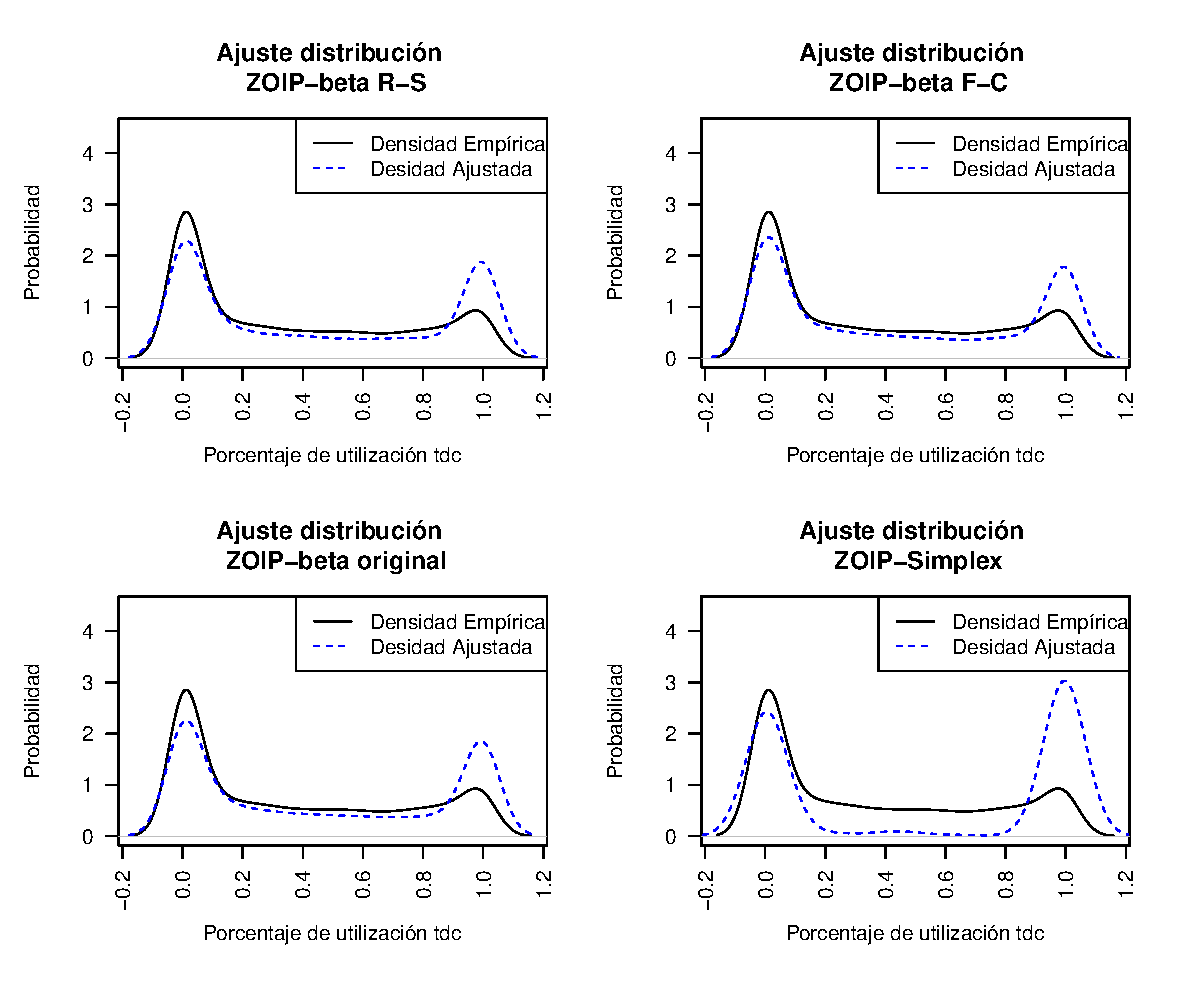
\includegraphics[scale=0.55]{Aplicacion_SC.eps}
		\caption{Ajuste de diferentes distribuciones y parametrizaciones ZOIP al porcentaje de utilizaci\'{o}n de una tdc.}
		\label{Apli_Aju_ZOIP}
	\end{center}
\end{figure}


En la Figura \ref{Apli_Aju_ZOIP} se presenta gr\'{a}ficamente el ajuste de la distribuci\'{o}n ZOIP para diferentes parametrizaciones al porcentaje de utilizaci\'{o}n de las tdc, la l\'{\i}nea azul que representa la distribuci\'{o}n ZOIP ajustada, es de notar que dicha l\'{\i}nea azul es exactamente igual en las tres ocasiones que se ajusta la distribuci\'{o}n ZOIP-beta y se ve como sigue el comportamiento original del porcentaje de utilizaci\'{o}n de las tdc. Es bueno resaltar tambi\'{e}n como en la Figura 1d de la Figura \ref{Apli_Aju_ZOIP} no se nota un buen ajuste para los valores entre cero y uno. Por todo anterior es recomendable decir que el porcentaje de utilizaci\'{o}n de las tdc de este banco se comportan como una distribuci\'{o}n ZOIP-beta con los par\'{a}metros descritos en la tabla \ref{T_Apli_SC}, seg\'{u}n la parametrizaci\'{o}n deseada y no como una distribuci\'{o}n ZOIP-simplex.

%%%%%%%%%%%%%%%%%%%%%%%%%%%%%%%%%%%%%%%%%%%%%%%%%%%%%%%%%%%%%%%%%%%%%%%%%%%%%%%%%%%%%%%%%%%%%%%%%%%%%%%%%%%%%%%%%%%%%%%%%%%%%%%%%%%%%%%%%%%%%%%%%%%%%%%%%%%%%%%%%%

\section{Conclusiones}

La distribuci\'{o}n ZOIP y el paquete \pkg{ZOIP} de \proglang{R} permiten ajustar distribuciones para datos provenientes de porcentajes, tasas o proporciones que se encuentren inflados con ceros y/o unos, dicha distribuci\'{o}n est\'{a} compuesta por cuatro par\'{a}metros, que son estimados v\'{\i}a m\'{a}xima verosimilitud y en el cual de acuerdo a los estudios de simulaci\'{o}n realizados estos convergen a los valores reales con un tama\~{n}o de muestra relativamente peque\~{n}o, adem\'{a}s se observa como la estimaci\'{o}n de los par\'{a}metros de la parte continua no se ven afectados por el aumento de la presencia de ceros y unos en los datos, pero si la estimaci\'{o}n de los par\'{a}metros de la parte discreta. Por otra parte, se observa como el Ajuste de la distribuci\'{o}n ZOIP-beta explica el comportamiento de la distribuci\'{o}n del porcentaje de utilizaci\'{o}n de una tarjeta de cr\'{e}dito en un banco.\\

La distribuci\'{o}n ZOIP y el paquete \pkg{ZOIP} de \proglang{R} permiten de una manera muy vers\'{a}til utilizar y ajustar diferentes parametrizaciones y distribuciones para datos proporcionales. Adem\'{a}s permite Utilizar y ajustar distribuciones para datos proporcionales que se encuentran inflados solo con ceros o solo con unos, de una manera pr\'{a}ctica.

\chapter{Cap\'{\i}tulo 3: Modelo de regresi\'{o}n ZOIP con efectos fijos}\label{cap3}
%{\Huge \textbf{Modelo de regresi\'{o}n ZOIP con efectos fijos\\}}
%Los datos obtenidos a partir de variables medidas bajo porcentajes, tasas y proporciones, son llamados datos proporcionales y estos se encuentran ubicados por lo general en el intervalo (0,1), sin embargo existen casos de este tipo de variables pueden dar resultados de cero y/o uno, representando la ausencia o presencia total de la caracter\'{\i}stica medida a partir de una variable, este tipo de datos son conocidos como datos proporcionales inflados con ceros y/o unos, existen diferentes distribuciones que explican estos datos, tales como la distribuci\'{o}n beta inflada con ceros o unos \citep{Ospina2} o de una manera m\'{a}s general la distribuci\'{o}n ZOIP (Zeros Ones inflated Proportional) que busca reunir la distribuci\'{o}n simplex y beta bajo diferentes parametrizaciones en una sola distribuci\'{o}n.\\

En muchos casos de estudio es razonable preguntarse c\'{o}mo puede ser explicada una variable aleatoria proveniente de datos proporcionales a partir de diferentes covariables, el modelo m\'{a}s conocido en la literatura para abordar este problema es la regresi\'{o}n beta, \cite{Paolino1} estima mediante el m\'{e}todo de m\'{a}xima verosimilitud, los par\'{a}metros para una regresi\'{o}n beta con parametrizaci\'{o}n original, \cite{Ferrari2} reparametrizan la distribuci\'{o}n y proponen el modelo regresi\'{o}n beta bajo esta nueva parametrizaci\'{o}n, luego \cite{Zeileis1} crean el paquete \pkg{betareg} de \proglang{R} en el cual se implementa dicha regresi\'{o}n. Por otro parte, \cite{Stasinopoulos2} tambi\'{e}n realizaron otra reparametrizaci\'{o}n de la distribuci\'{o}n beta original, en terminos de la media y la dispersi\'{o}n, adem\'{a}s introducen un modelo de regresi\'{o}n beta basado en dicha distribuci\'{o}n y lo implementan en el paquete \pkg{gamlss} de \proglang{R}. Existe otro modelo de regresi\'{o}n basado en  la distribuci\'{o}n simplex, propuesta por \cite{Barndorff1}, este nuevo modelo de regresi\'{o}n fue realizada por \cite{Qiu1} e implementado en el paquete \pkg{simplexreg}, \cite{Zhang1}.\\

Sin embargo, los anteriores modelos de regresi\'{o}n son realizados para datos proporcionales no inflados con ceros o unos, es por esto que \cite{Ospina1} propusieron un modelo de regresi\'{o}n inflado con cero o con uno (no con ambos) bajo la distribuci\'{o}n beta inflada de \cite{Ospina2} y bajo la parametrizaci\'{o}n \cite{Ferrari2}, de igual manera \cite{Stasinopoulos2} implementan los modelos de regresi\'{o}n beta inflados con ceros y/o unos, y se encuentran implementados en el paquete \pkg{gamlss} de \proglang{R} \citep{Stasinopoulos1}, sin embargo, para la utilizaci\'{o}n del modelo de regresi\'{o}n inflado solo con ceros o unos o con ambos, se deben utilizar funciones distintas dentro del paquete para ajustar los tres diferentes modelos de regresi\'{o}n. Adem\'{a}s no existen paquetes en \proglang{R} que logren ajustar un modelo de regresi\'{o}n beta inflado con ceros y/o unos bajo las parametrizaciones originales y de \cite{Ferrari2}, por otra parte a pesar de que existen desarrollos te\'{o}ricos sobre el modelo de regresi\'{o}n simplex inflado con ceros y/o unos \citep{Galvis1}, no existe un paquete en \proglang{R} que permita realizar un ajuste sobre dicho modelo de regresi\'{o}n.\\

Es por esto que en este trabajo se implementa de manera te\'{o}rica y de forma pr\'{a}ctica mediante el paquete \pkg{ZOIP} en el sistema de computaci\'{o}n \proglang{R} \citep{R} y disponible en el repositorio web \verb|GitHub|, un modelo de regresi\'{o}n para datos proporcionales inflados con ceros y/o unos (Modelo de regresi\'{o}n ZOIP) que permita mediante una misma funci\'{o}n ajustar mo\-de\-los en diferentes distribuciones para datos proporcionales y en diferentes parametrizaciones.\\

Este cap\'{\i}tulo se encuentra organizado de la siguiente manera: primero se presenta el modelo de regresi\'{o}n ZOIP que es basado en la distribucion ZOIP visto en el cap\'{\i}tulo anterior y su debida estimaci\'{o}n, mediante maxima verosimilitud, en la siguiente secci\'{o}n se presenta la implementaci\'{o}n del modelo de regresi\'{o}n ZOIP en el paquete \pkg{ZOIP} de \proglang{R} y por \'{u}ltimo se presentan unas aplicaciones a datos simulados y a datos reales.


%%%%%%%%%%%%%%%%%%%%%%%%%%%%%%%%%%%%%%%%%%%%%%%%%%%%%%%%%%%%%%%%%%%%%%%%%%%%%%%%%%%%%%%%%%%%%%%%%%%%%%%%%%%%%%%%%%%%%%%%%%%%%%%%%%%%%%%%%%%%%%%%%%%%%%%%%%%%%%%%%%

\section{Modelo de regresi\'{o}n ZOIP}

Una clase general de modelos de regresi\'{o}n ZOIP puede definirse como sigue. Sea $y_1, y_2,\ldots, y_n$ variables aleatorias independientes tal que cada $y_i$, para $i=1,\ldots, n$, tiene funci\'{o}n de densidad de probabilidad \eqref{eq_Dist_ZOIP} con par\'{a}metros $\mu = \mu_i$, $\sigma=\sigma_i$, $p_0=p_{0i}$, y $p1=p_{1i}$. Se asume que $\mu_i$, $\sigma_i$, $p_{0i}$ y $p_{1i}$ se definen como

\begin{equation}
\begin{split}
&h_1(\mu_{i})=\mathbf{x}_{i1}^{\top} \boldsymbol{\beta}_1,\\
&h_2(\sigma_{i})=\mathbf{x}_{i2}^{\top} \boldsymbol{\beta}_2,\\
&h_3(p_{0i})=\mathbf{x}_{i3}^{\top} \boldsymbol{\beta}_3,\\
&h_4(p_{1i}) =\mathbf{x}_{i4}^{\top} \boldsymbol{\beta}_4
\end{split}
\label{eq_reg}
\end{equation}

donde $\mathbf{x}_{i1}=(x_{i11}, x_{i12},\ldots, x_{i1k_1})^{\top}$, $\mathbf{x}_{i2}=(x_{i21}, x_{i22},\ldots, x_{i2k_2})^{\top}$, \\
$\mathbf{x}_{i3}=(x_{i31}, x_{i32},\ldots, x_{i1k_3})^{\top}$ y $\mathbf{x}_{i4}=(x_{i41}, x_{i42},\ldots, x_{i1k_4})^{\top}$, son vectores de covariables conocidos de dimensi\'{o}n $k_1$, $k_2$, $k_3$ y $k_4$ respectivamente, $\boldsymbol{\beta}_1=(\beta_{11}, \beta_{12},\ldots, \beta_{1k_1})^{\top}$, \\
$\boldsymbol{\beta}_2=(\beta_{21}, \beta_{22},\ldots, \beta_{2k_2})^{\top}$, $\boldsymbol{\beta}_3=(\beta_{31}, \beta_{32},\ldots, \beta_{3k_3})^{\top}$ y $\boldsymbol{\beta}_4=(\beta_{41}, \beta_{42},\ldots, \beta_{4k_4})^{\top}$ son vectores de par\'{a}metros de regresi\'{o}n desconocidos. Adem\'{a}s se asume que las funciones de enlace $h_1(\cdot)$, $h_2(\cdot)$, $h_3(\cdot)$ y $h_4(\cdot)$ son conocidas y apropiadas para mapear de los reales a los valores admisibles del par\'{a}metro, ademas son funciones estrictamente mon\'{o}tonas y doblemente diferenciables. Las posibles funciones de enlace para el par\'{a}metro $\mu$ y $\sigma$ son logit, probit, clog-log, o log dependiendo de la parametrizaci\'{o}n, para los par\'{a}metros de inflaci\'{o}n $p_0$ y $p_1$ son posibles funciones de enlace como logit, probit, clog-log. Estudios sobre funciones enlace mal especificadas sobre modelos de regresi\'{o}n beta se encuentran en \cite{andrade07}.

\subsection{Inferencia estad\'{\i}stica}

Para estimar los par\'{a}metros del modelo de regresi\'{o}n ZOIP se usar\'{a} el m\'{e}todo de m\'{a}xima verosimilitud. La funci\'{o}n de verosimilitud para $\boldsymbol{\theta}=(\boldsymbol{\beta_1}^{\top},\boldsymbol{\beta_2}^{\top},\boldsymbol{\beta_3}^{\top}, \boldsymbol{\beta_4}^{\top})^{\top}$, basado en una muestra de observaciones independientes, es de la forma:

\begin{equation}
L(\boldsymbol{\theta})=\prod_{i=1}^{n}g(\mathbf{y}_i;\mu_i,\sigma_i,p_{0i},p_{1i})=\prod_{i=1}^{n}f_1(\mathbf{y}_i;p_{0i})\prod_{i=1}^{n}f_2(\mathbf{y}_i;p_{1i})\prod_{i=1}^{n}f_3(\mathbf{y}_i;\mu_i,\sigma_i)
\label{F_likel}
\end{equation}

%\[
%\ell(\boldsymbol{\theta})=\sum_{i=1}^{n}{\ell_i(\mu_i,\sigma_i,p_{0i},p_{1i}) }
%\]

donde para el caso de ZOIP-beta original $\mu_i=p_i$, $\sigma_i=q_i$; si la distribuci\'{o}n ZOIP-beta fuese con parametrizaci\'{o}n de \cite{Ferrari2} el \'{u}nico par\'{a}metro que cambiar\'{\i}a es $\sigma_i=\phi_i$, el resto de los par\'{a}metros no tendr\'{\i}an modificaciones seg\'{u}n su parametrizaci\'{o}n o distribuci\'{o}n.\\

La funci\'{o}n de verosimilitud definida en \eqref{F_likel} al aplicar logaritmo natural se obtiene la funci\'{o}n de log verosimilitud definida como:
\[
\ell(\boldsymbol{\theta})=\ell_1(\boldsymbol{\beta_3})+\ell_2(\boldsymbol{\beta_4})+\ell_3(\boldsymbol{\beta_1},\boldsymbol{\beta_2})
\]
\\
Note que la funci\'{o}n de verosimilitud es factorizada en tres t\'{e}rminos, dos de ellos del componente discreto y uno compuesto por $\boldsymbol{\beta_1}$ y $\boldsymbol{\beta_2}$ del componente continuo, por tanto los par\'{a}metros son separables \citep{Pace1}, as\'{\i} la m\'{a}xima verosimilitud puede ser tratada por separado y por lo tanto:\\
\begin{align*}
\begin{split}
	\ell_1(\boldsymbol{\beta_3}) &= \sum_{i=1}^{n}{p_{0i}^{S_0(y_i)}(1-p_{0i})^{1-S_0(y_i)}}
\end{split}\\
\begin{split}
	\ell_2(\boldsymbol{\beta_4}) &= \sum_{i=1}^{n}{p_{1i}^{S_1(y_i)}(1-p_{1i})^{1-S_1(y_i)}}
\end{split}\\
\begin{split}
	\ell_3(\boldsymbol{\beta_1},\boldsymbol{\beta_2}) &= \sum_{i=1:y_i \in (0,1)}^{n}{f_3(y_i;\mu_i,\sigma_i)} 
\end{split}
\end{align*}

Con
\[
S_j(y_i)=
\begin{cases}
1 & \text{si}\ y_i=j\\
0 & \text{si}\ y_i\neq j\\
\end{cases}
\quad ; \quad j=1,2
\]
\\
Con $p_{0i}=h_3^{-1}(\mathbf{x}_{i3}^{\top} \boldsymbol{\beta}_3)$, $p_{1i}=h_4^{-1}(\mathbf{x}_{i4}^{\top} \boldsymbol{\beta}_4)$, $\mu_i=h_1^{-1}(\mathbf{x}_{i1}^{\top} \boldsymbol{\beta}_1)$ y $\sigma_i=h_2^{-1}(\mathbf{x}_{i2}^{\top} \boldsymbol{\beta}_2)$ como se defini\'{o} en \eqref{eq_reg}. La funcion de verosimilitud depende de tres terminos, el primero depende de $\boldsymbol{\beta}_3$ (componente discreto para inflaci\'{o}n en cero), el segundo de $\boldsymbol{\beta}_4$ (componente discreto para explicar la inflaci\'{o}n en uno) y el tercero depende de $(\boldsymbol{\beta}_1,\boldsymbol{\beta}_2)$ (Componentes para explicar la parte continua), por lo tanto los par\'{a}metros son separables y la inferencia de m\'{a}xima verosimilitud para $\boldsymbol{\beta}_1$ y $\boldsymbol{\beta}_2$ se puede hacer por separado de la de $\boldsymbol{\beta}_3$ y $\boldsymbol{\beta}_4$, como si conociera a $\boldsymbol{\beta}_3$ y $\boldsymbol{\beta}_4$ y viceversa. \citep{Ospina1}.\\

No existen expresiones que den una soluci\'{o}n cerrada anal\'{\i}ticamente para encontrar los m\'{a}ximos de las funciones de log verosimilitudes descritas anteriormente, para as\'{\i} hallar los estimadores de m\'{a}xima verosimilitud de los par\'{a}metros de regresi\'{o}n de cada uno de los componentes de la distribuci\'{o}n ZOIP. Por lo que es necesario utilizar algoritmos de optimizaci\'{o}n no lineal como el m\'{e}todo de Newton-Raphson o Fisher's scoring, para nuestro caso utilizaremos el algoritmo de optimizaci\'{o}n dado por la funci\'{o}n \code{nlminb} o \code{optim} del paquete \code{stats} de \proglang{R} e implementado en el paquete \pkg{ZOIP} de \proglang{R} para el modelo de regresi\'{o}n ZOIP.

%%%%%%%%%%%%%%%%%%%%%%%%%%%%%%%%%%%%%%%%%%%%%%%%%%%%%%%%%%%%%%%%%%%%%%%%%%%%%%%%%%%%%%%%%%%%%%%%%%%%%%%%%%%%%%%%%%%%%%%%%%%%%%%%%%%%%%%%%%%%%%%%%%%%%%%%%%%%%%%%%%

\section{Modelo de regresi\'{o}n ZOIP en el Paquete \pkg{ZOIP}}

En esta secci\'{o}n presentaremos como el paquete \pkg{ZOIP} realizado en \proglang{R} ajusta un modelo de regresi\'{o}n ZOIP con efectos fijos, v\'{\i}a m\'{a}xima verosimilitud.

%\subsection{Instalaci\'{o}n}
%
%La versi\'{o}n m\'{a}s actualizada del paquete \pkg{ZOIP} se encuentra ubicada en \verb|GitHub|, el cual es un alojamiento de repositorios Git, para obtener dicha versi\'{o}n es necesario ejecutar el siguiente c\'{o}digo que instala el devtools que es necesario para descargar el paquete \pkg{ZOIP}.
%
%\begin{verbatim}
%if (!require('devtools')) install.packages('devtools')
%devtools::install_github('jucdiaz/ZOIP', force=TRUE)
%require(ZOIP)  # Carga el paquete
%\end{verbatim}

\subsection{Funci\'{o}n RM.ZOIP}

La funci\'{o}n \code{RM.ZOIP} estima los par\'{a}metros de un modelo de regresi\'{o}n ZOIP con y sin covariables v\'{\i}a m\'{a}xima verosimilitud utilizando el optimizador \code{nlminb} o \code{optim}. La estructura de la funci\'{o}n \code{RM.ZOIP} es la siguiente:

\begin{verbatim}
RM.ZOIP(formula.mu, formula.sigma = ~1, formula.p0 = ~1, 
    formula.p1 = ~1, data, link = c("identity", "identity", 
        "identity", "identity"), family = "R-S", optimizer = "nlminb")
\end{verbatim}

Los argumentos de la funci\'{o}n \code{RM.ZOIP} son:

\begin{itemize}[noitemsep, nolistsep]

\item \code{formula.mu}: f\'{o}rmula que define la variable respuesta y la estructura de covariables para modelar el par\'{a}metro $\mu$, por ejemplo si se escribe \code{y $\sim$ x1 + x2} significa que la variable respuesta es $y$ y que $h(\mu)=\beta_0 + \beta_1 x_1 + \beta_2 x_2$.
\item \code{formula.sigma}: f\'{o}rmula que define la funci\'{o}n de regresi\'{o}n de efectos fijos, para el par\'{a}metro $\sigma$, un valor posible es \code{$\sim$ x1}, por defecto \code{$\sim$ 1}.
\item \code{formula.p0}: f\'{o}rmula que define la funci\'{o}n de regresi\'{o}n de efectos fijos, para el par\'{a}metro $p_0$, un valor posible es \code{$\sim $x1}, por defecto \code{$\sim $1}.
\item \code{formula.p1}: f\'{o}rmula que define la funci\'{o}n de regresi\'{o}n de efectos fijos, para el par\'{a}metro $p_1$, un valor posible es \code{$\sim $x1}, por defecto \code{$\sim $1}.
\item \code{data}: es el conjunto de datos en formato \code{data.frame} donde deben estar las variables tal cual como est\'{a}n en las f\'{o}rmulas.
\item \code{family}: elecci\'{o}n de la parametrizaci\'{o}n de la distribuci\'{o}n beta o distribuci\'{o}n deseada en la parte continua de la distribuci\'{o}n ZOIP. El valor de \code{``R-S''} indicar\'{a} la distribuci\'{o}n beta con parametrizaci\'{o}n \cite{Stasinopoulos2}, si toma el valor de \code{``F-C''} se utilizar\'{a} la distribuci\'{o}n beta parametrizaci\'{o}n \cite{Ferrari2}, el valor de \code{``Original''} se utilizar\'{a} la distribuci\'{o}n beta con parametrizaci\'{o}n original, \code{``Simplex''} utilizar\'{a} la distribuci\'{o}n simplex.
\item \code{link}: es un vector con las funciones enlace adecuadas para cada par\'{a}metro a estimar de acuerdo a las opciones escogidas en los par\'{a}metros de familia y f\'{o}rmula. Si la funci\'{o}n de regresi\'{o}n no posee covariables para la explicaci\'{o}n de los par\'{a}metros de $\mu$, $\sigma$, $p_0$ o $p_1$; entonces se debe utilizar como funci\'{o}n enlace la opci\'{o}n \code{identity}, independientemente de la parametrizaci\'{o}n deseada (familia). Los posibles valores para las funciones enlace son \code{identity}, \code{logit} y \code{log}.\\
Por defecto \code{link=c(``identity'',``identity'',``identity'',``identity'')}.
\item \code{optimizer}: elecci\'{o}n del optimizador, utilizado para encontrar la convergencia de la m\'{a}xima verosimilitud en los par\'{a}metros de efectos fijos, se puede elegir el valor de \code{``nlminb''} u \code{``optim''}, por defecto \code{``nlminb''}.


\end{itemize}

En el siguiente ejemplo nos concentraremos en el ajuste de un modelo regresi\'{o}n ZOIP, para ello se mostrar\'{a} el c\'{o}digo utilizado y la salida de la funci\'{o}n \code{RM.ZOIP}, para una variable aleatoria simulada de una distribuci\'{o}n ZOIP-beta con parametrizaci\'{o}n \cite{Stasinopoulos2} y dos covariables simuladas a partir de una distribuci\'{o}n uniforme entre cero y uno, el tama\~{n}o de la muestra simulada es 1000. Esto replicando exactamente uno de los casos de simulaci\'{o}n vistos en la pr\'{o}xima secci\'{o}n.\\

Primero se simula la variable respuesta a partir de la funci\'{o}n \code{rZOIP} con los debidos valores de los par\'{a}metros para cada observaci\'{o}n, y las covariables.

\begin{verbatim}
library(ZOIP)
n <- 1000
x1 <- runif(n)
x2 <- runif(n)

c1 <- 0.2
c2 <- -1
mu_i <- inv.logit(c1 + c2 * x1)

b1 <- 0.3
b2 <- 3
b3 <- 0.9
sigma_i <- inv.logit(b1 + b2 * x1 + b3 * x2)
\end{verbatim}
\begin{verbatim}
d1 <- 0.07
p0_i <- rep(d1, n)

e1 <- 0.02
e2 <- -4
p1_i <- inv.logit(e1 + e2 * x2)

param <- cbind(mu_i, sigma_i, p0_i, p1_i)
y_i <- apply(param, 1, function(x)
{
    rZOIP(1, mu = x[1], sigma = x[2], p0 = x[3], p1 = x[4], 
        family = "R-S")
})

data <- as.data.frame(cbind(y_i, x1, x2))

link <- c("logit", "logit", "identity", "logit")
mod <- RM.ZOIP(formula.mu = y_i ~ x1, formula.sigma = ~x1 + 
    x2, formula.p0 = ~1, formula.p1 = ~x2, data = data, 
    link = link, family = "R-S")

mod
\end{verbatim}

Los resultados obtenidos se muestran a continuaci\'{o}n.

\begin{verbatim}
## Call:
## RM.ZOIP(formula.mu = y_i ~ x1, formula.sigma = ~x1 + x2, formula.p0 = ~1, 
##     formula.p1 = ~x2, data = data, link = link, family = "R-S")
## 
##  Results: 
## 
##  Estimated coefficients for h(mu): 
## (Intercept)          x1 
##   0.3395118  -1.4808985 
## 
\end{verbatim}
\begin{verbatim}
##  Estimated coefficients for h(sigma): 
## (Intercept)          x1          x2 
##   0.7006753   2.4493508   0.5328350 
## 
##  Estimated coefficients for h(p0): 
## (Intercept) 
##  0.08199999 
## 
##  Estimated coefficients for h(p1): 
## (Intercept)          x2 
##  -0.1252807  -3.0092159 
## 
##  Convergence 
## [1] 0
## 
##  message 
## [1] "relative convergence (4)"
## 
##  iterations 
## [1] 39
## 
##  Log-likelihood 
## [1] 7688.628
\end{verbatim}

En el anterior resultado se obtienen varios aspectos importantes de la salida del modelo y leyendo de arriba hacia abajo, primero que todo nos muestra el modelo ajustado, luego para cada par\'{a}metro de la distribuci\'{o}n ZOIP los valores estimados para cada uno de los pa\-r\'{a}\-me\-tros de regresi\'{o}n asociados a cada covariable, luego un indicador de convergencia, donde 0 indica la convergencia, despu\'{e}s un mensaje sobre la convergencia (resultados heredados de la funci\'{o}n \code{nlimnb}), despu\'{e}s se encuentra el n\'{u}mero de iteraciones que fueron necesarias para que convergiera el modelo, por \'{u}ltimo se encuentra valor de la log-verosimilitud que nos permitir\'{a} hacer comparaciones entre modelos.\\ 

 Al aplicar al modelo ajustado (\code{mod}) la funci\'{o}n \code{summary} se obtiene el siguiente resultado:

\begin{verbatim}
summary(mod)
## ---------------------------------------------------------------
## Fixed effects for logit(mu) 
## ---------------------------------------------------------------
##              Estimate Std. Error z value  Pr(>|z|)    
## (Intercept)  0.339512   0.098754  3.4379 0.0005862 ***
## x1          -1.480898   0.179015 -8.2725 < 2.2e-16 ***
## ---
## Signif. codes:  0 *** 0.001 ** 0.01 * 0.05 . 0.1   1
## ---------------------------------------------------------------
## Fixed effects for logit(sigma) 
## ---------------------------------------------------------------
##             Estimate Std. Error z value  Pr(>|z|)    
## (Intercept)  0.70068    0.10726  6.5323 6.476e-11 ***
## x1           2.44935    0.13775 17.7812 < 2.2e-16 ***
## x2           0.53283    0.13273  4.0143 5.961e-05 ***
## ---
## Signif. codes:  0 *** 0.001 ** 0.01 * 0.05 . 0.1   1
## ---------------------------------------------------------------
## Fixed effects for identity(p0) 
## ---------------------------------------------------------------
##              Estimate Std. Error z value  Pr(>|z|)    
## (Intercept) 0.0820000  0.0086762  9.4512 < 2.2e-16 ***
## ---
## Signif. codes:  0 *** 0.001 ** 0.01 * 0.05 . 0.1   1
## ---------------------------------------------------------------
## Fixed effects for logit(p1) 
## ---------------------------------------------------------------
##             Estimate Std. Error z value Pr(>|z|)    
## (Intercept) -0.12528    0.15084 -0.8305   0.4062    
## x2          -3.00922    0.34242 -8.7881   <2e-16 ***
## ---
## Signif. codes:  0 *** 0.001 ** 0.01 * 0.05 . 0.1   1
## ---------------------------------------------------------------
## ---------------------------------------------------------------
\end{verbatim}

Con la funci\'{o}n \code{summary} aplicada al modelo de regresi\'{o}n ZOIP, se obtiene m\'{a}s detalles de los par\'{a}metros regresores estimados para cada par\'{a}metro del modelo de regresi\'{o}n ZOIP, se obtiene el valor estimado (Estimate), su error est\'{a}ndar (Std.Error), el valor Z del estimador (z value) y el valor p que nos indicara la significancia del par\'{a}metro estimado (\code{Pr(>|z|)}), es de notar que para cada par\'{a}metro del modelo de regresi\'{o}n ZOIP le es mostrado la respectiva funci\'{o}n enlace utilizada y definida al inicio del modelo.
%%%%%%%%%%%%%%%%%%%%%%%%%%%%%%%%%%%%%%%%%%%%%%%%%%%%%%%%%%%%%%%%%%%%%%%%%%%%%%%%%%%%%%%%%%%%%%%%%%%%%%%%%%%%%%%%%%%%%%%%%%%%%%%%%%%%%%%%%%%%%%%%%%%%%%%%%%%%%%%%%%

\section{Aplicaci\'{o}n}
En esta secci\'{o}n se muestran diferentes resultados sobre el ajuste de un modelo de regresi\'{o}n ZOIP, por medio del paquete \pkg{ZOIP}, primero se realiz\'{o} un estudio de simulaci\'{o}n para analizar la convergencia de la estimaci\'{o}n de los par\'{a}metros regresores de una regresi\'{o}n ZOIP, y en segunda instancia se ajusta un modelo de regresi\'{o}n ZOIP a datos reales, sobre c\'{o}mo puede ser explicado el porcentaje de utilizaci\'{o}n de una tarjeta de cr\'{e}dito (tdc) de una entidad financiera con diferentes variables del negocio.

\subsection{Datos simulados}
En el estudio de simulaci\'{o}n se analizan diferentes aspectos de la capacidad de estimaci\'{o}n que tiene el m\'{e}todo de m\'{a}xima verosimilitud sobre los par\'{a}metros regresores de un modelo de regresi\'{o}n ZOIP. Para comprobar esto se generaron muestras pertenecientes a una distribuci\'{o}n ZOIP a partir de dos variables aleatorias uniformes cero uno, con tama\~{n}os de muestra de 25, 50, 75, y 100 a partir de este punto no se realizar\'{a}n incrementos de 25 si no de 100, es decir 100, 200, 300 hasta 3500, y se realizaron 1000 r\'{e}plicas para cada tama\~{n}o de muestra, posteriormente se calcul\'{o} la mediana de la estimaci\'{o}n de cada par\'{a}metro regresor para cada distribuci\'{o}n y parametrizaci\'{o}n utilizada. A continuaci\'{o}n, se muestra la estructura simulada para cada par\'{a}metro de la distribuci\'{o}n ZOIP.\\

Si $y_{i} \sim ZOIP(\mu_{i},\sigma_{i},p_{0i}, p_{1i}),$

\begin{equation}
\begin{split}
&h_1(\mu_{i})=\beta_0+\beta_1x_{1i},\\
&h_2(\sigma_{i})=\beta_0+\beta_1x_{1i}+\beta_2x_{2i},\\
&h_3(p_{0i})=\beta_0,\\
&h_4(p_{1i}) =\beta_0+\beta_1x_{2i},
\end{split}
\label{S_eq_reg}
\end{equation}

donde para la regresi\'{o}n de $\mu$: $\beta_0=0.2$ y $\beta_1=-1$, para la de $\sigma$ se escogieron dos escenarios distintos si la regresi\'{o}n a modelar es ZOIP-beta parametrizaci\'{o}n de \cite{Stasinopoulos2}, entonces: $\beta_0=0.3$, $\beta_1=-2$, $\beta_2=-4$, para las dem\'{a}s parametrizaci\'{o}n y distribuciones $\beta_0=0.3$, $\beta_1=3$, $\beta_2=0.9$, esto para tener una variabilidad de los datos moderada. Para el par\'{a}metro $p_0$: $\beta_0=0.07$ y para $p_1$: $\beta_0=0.02$ y $\beta_1=-4$ para todos los casos posibles de selecci\'{o}n de la regresi\'{o}n ZOIP, y $x_{1i} \sim U(0,1)$, $x_{2i} \sim U(0,1)$. Las funciones de enlace adecuadas para cada distribuci\'{o}n y parametrizaci\'{o}n se muestran en la tabla \ref{T_F_enlace}.\\

\begin{table}[!hbt]
{\scriptsize
\begin{center}
\begin{tabular}{|c|c|c|}\hline
Familia & Par\'{a}metro & $h(\cdot)$ \\ \hline
\multirow{4}{*}{R-S} & $\mu$ & Logit \\
 & $\sigma$ & Logit \\
 & $p_0$ & NA \\
 & $p_1$ & Logit \\ \hline

\multirow{4}{*}{F-C} & $\mu$ & Logit \\
 & $\sigma$ & Log. \\
 & $p_0$ & NA \\
 & $p_1$ & Logit \\ \hline

\multirow{4}{*}{original} & $\mu$ & Log. \\
 & $\sigma$ & Log. \\
 & $p_0$ & NA \\
 & $p_1$ & Logit \\ \hline

\multirow{4}{*}{simplex} & $\mu$ & Logit \\
 & $\sigma$ & Log. \\
 & $p_0$ & NA \\
 & $p_1$ & Logit \\ \hline

\end{tabular}
\caption{Funciones de enlace adecuadas para cada par\'{a}metro, seg\'{u}n su distribuci\'{o}n y/o parametrizaci\'{o}n.}
\label{T_F_enlace}
\end{center}
}
\end{table}

\begin{figure}
	\begin{center}
		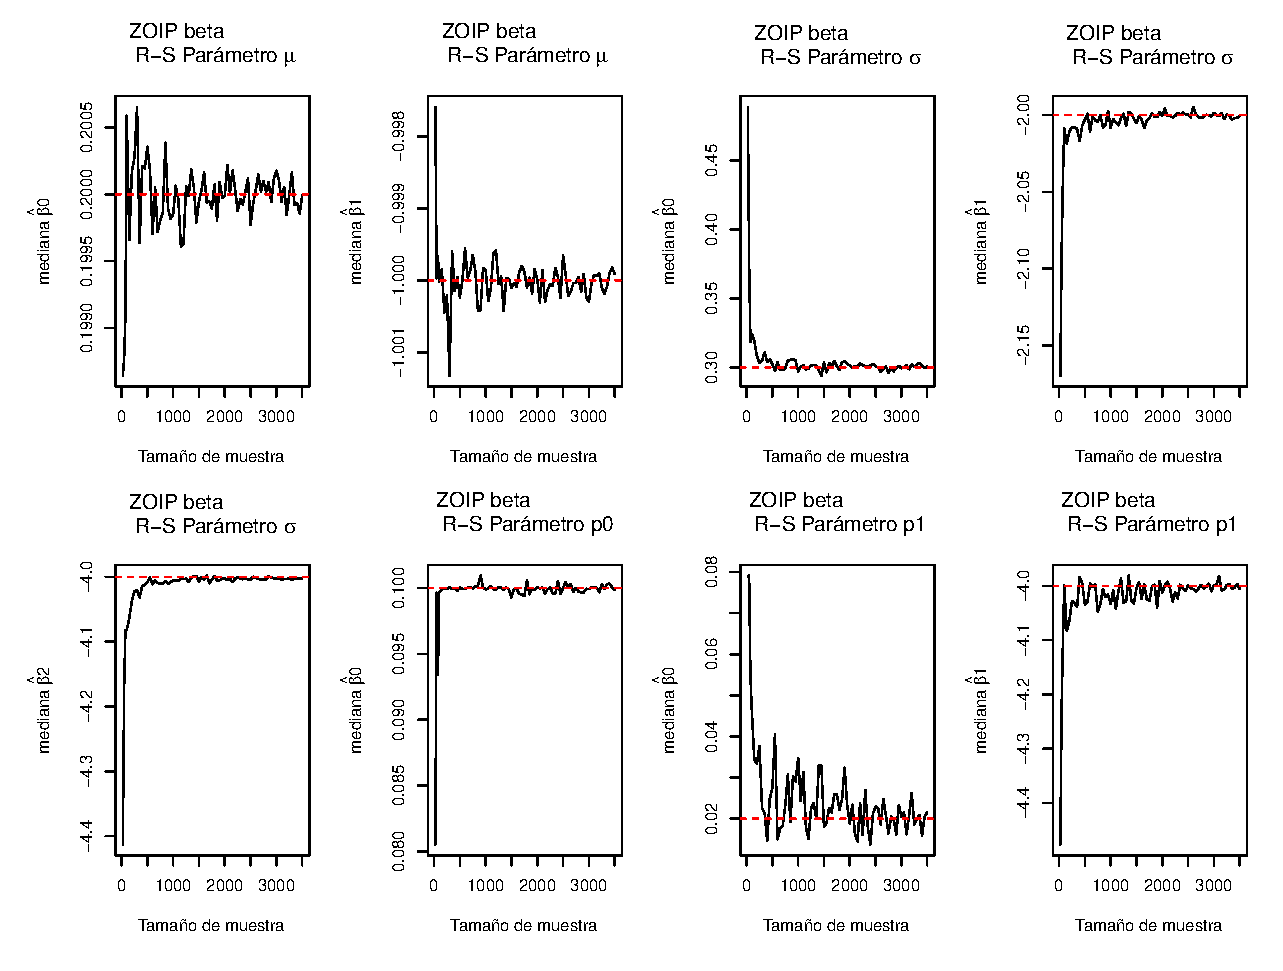
\includegraphics[scale=0.5]{Converg_RS.eps}	
		\caption{Simulaci\'{o}n de un modelo de regresi\'{o}n ZOIP-beta para la parametricazion R-S con diferentes valores de $n$.}
		\label{Simu_RS}
	\end{center}
\end{figure}

En la figura \ref{Simu_RS} se describen los valores estimados para diferentes valores de tama\~{n}o de muestra, cuando se elige realizar una regresi\'{o}n ZOIP-beta con parametrizaci\'{o}n de \cite{Stasinopoulos2}, en ella se ve como todos los par\'{a}metros estimados oscilan alrededor del valor real del par\'{a}metro que es representado por la l\'{\i}nea roja, sin embargo, se nota como unos par\'{a}metros tienen una oscilaci\'{o}n mayor que otros, como es el caso de los par\'{a}metros de intercepto de la media y el del par\'{a}metro de inflaci\'{o}n de unos, asociada a $p_1$. Los de m\'{a}s par\'{a}metros convergen r\'{a}pidamente a sus valores reales, como los par\'{a}metros que representan la variabilidad ($\sigma$) y el par\'{a}metro de $p_0$.\\

\begin{figure}
	\begin{center}
		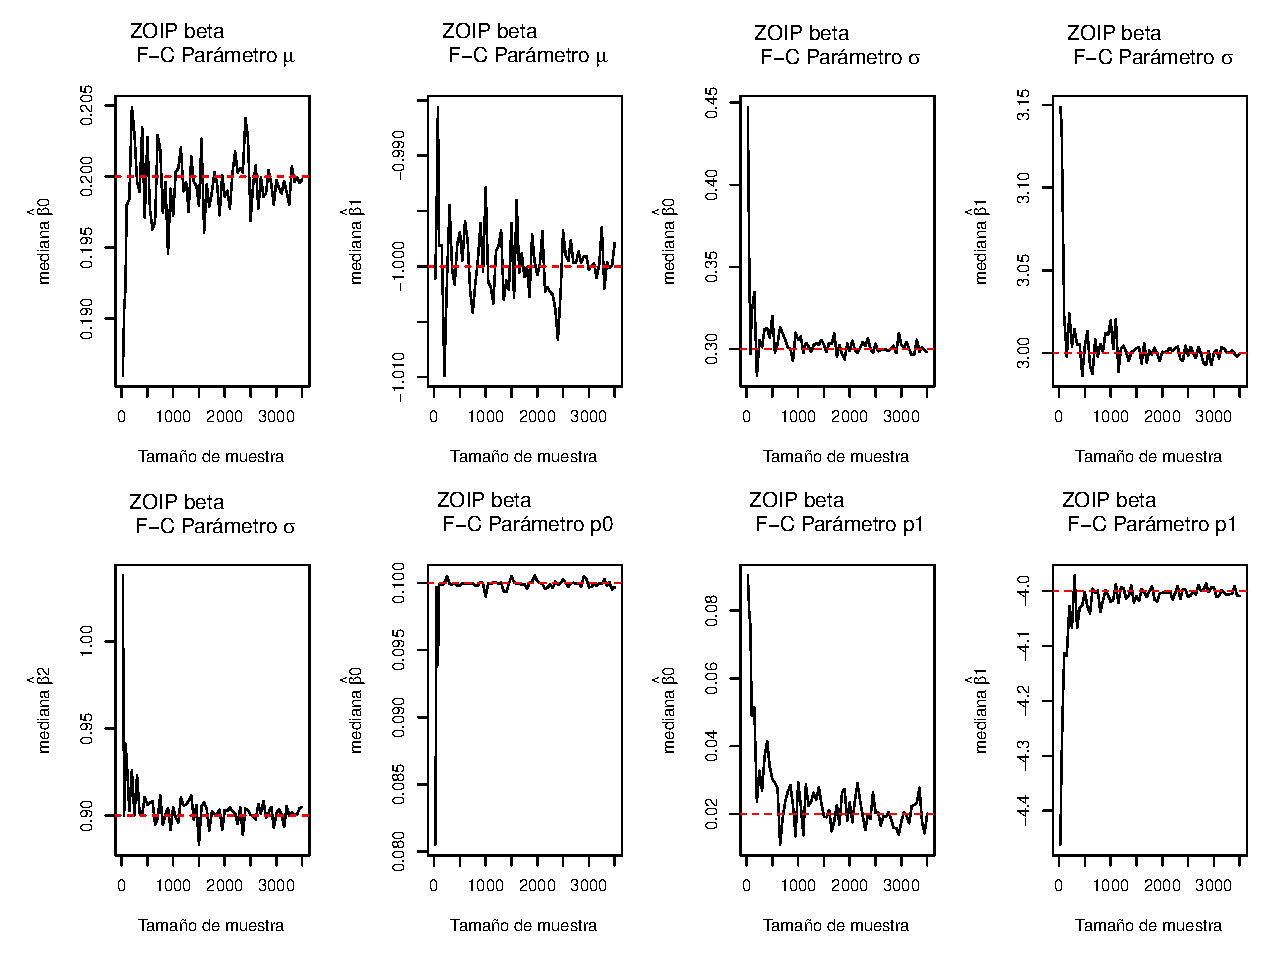
\includegraphics[scale=0.5]{Converg_FC.eps}	
		\caption{Simulaci\'{o}n de un modelo de regresi\'{o}n ZOIP-beta para la parametricazion F-C con diferentes valores de $n$.}
		\label{Simu_FC}
	\end{center}
\end{figure}

En la figura \ref{Simu_FC} se describen los valores estimados para diferentes tama\~{n}os de muestra, cuando se elige realizar una regresi\'{o}n ZOIP-beta con parametrizaci\'{o}n de \cite{Ferrari2}, en dicha figura se nota como la estimaci\'{o}n de los par\'{a}metros asociados con la media tienen una oscilaci\'{o}n mayor que los dem\'{a}s par\'{a}metros, sin embargo, en todos los par\'{a}metros se obsserva como a medida que el tama\~{n}o de muestra es m\'{a}s grande la oscilaci\'{o}n de los par\'{a}metros es menor y van convergiendo satisfactoriamente a sus valores reales.\\

\begin{figure}
	\begin{center}
		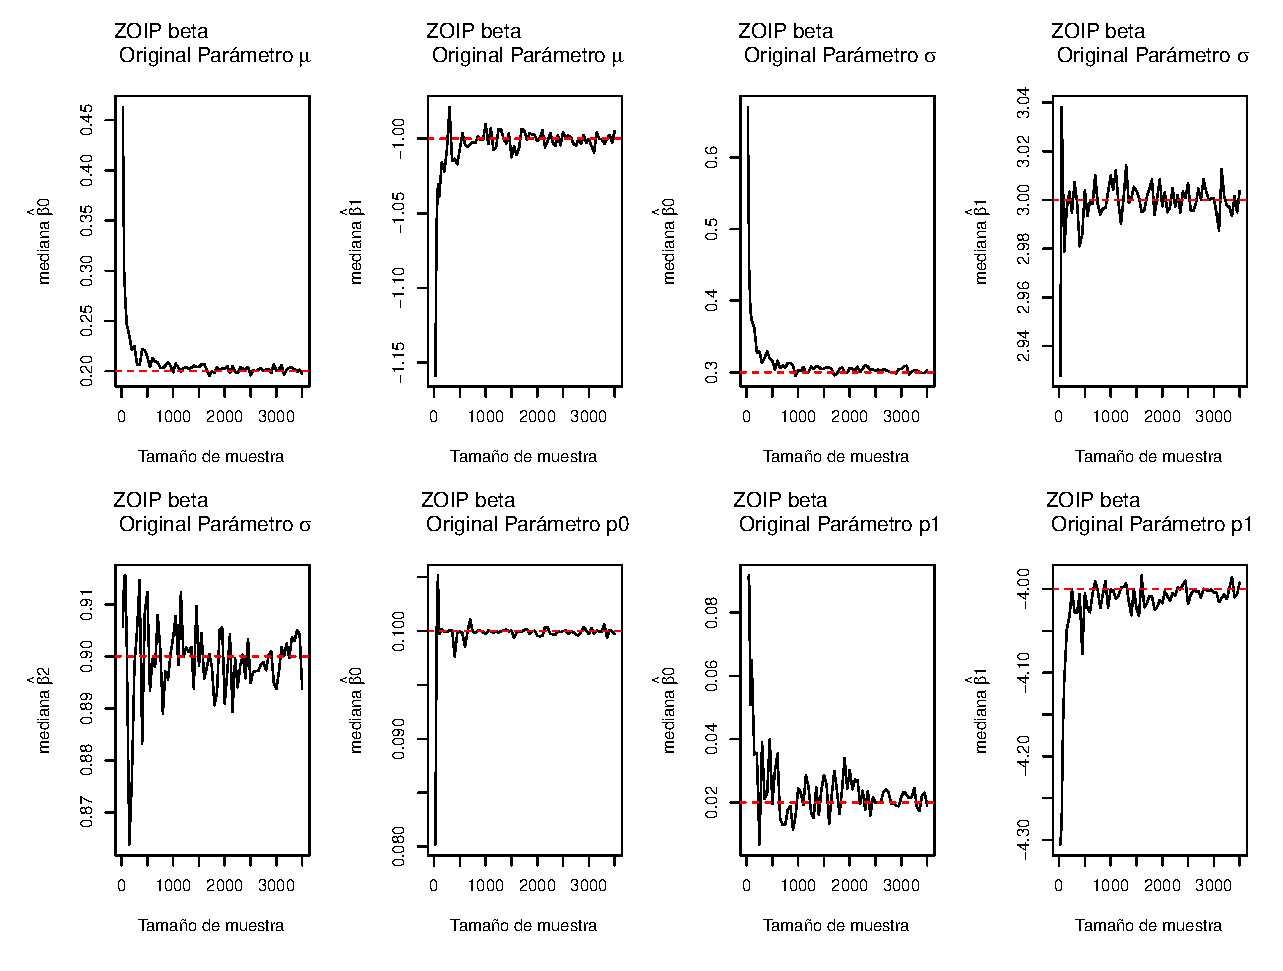
\includegraphics[scale=0.5]{Converg_Ori.eps}	
		\caption{Simulaci\'{o}n de un modelo de regresi\'{o}n ZOIP-beta para la parametricazion ori\-gi\-nal con diferentes valores de $n$.}
		\label{Simu_Ori}
	\end{center}
\end{figure}

En la figura \ref{Simu_Ori} se describen los valores estimados para diferentes tama\~{n}os de muestra, cuando se elige realizar una regresi\'{o}n ZOIP-beta con parametrizaci\'{o}n original, se puede ver como con los valores del escenario de simulaci\'{o}n elegidos, se obtiene una distribuci\'{o}n ZOIP con mayor variabilidad, por lo que los valores de los par\'{a}metros asociados a $\sigma$ tienen una mayor oscilaci\'{o}n, sin embargo, este oscila solo en un 0.01 de sus unidades, lo que no es preocupante. Por otra parte, se observa como el par\'{a}metro de intercepto del par\'{a}metro de inflaci\'{o}n de unos ($p_1$) si oscila mucho m\'{a}s ya que este tiene una desviaci\'{o}n est\'{a}ndar de 0.04 en promedio, pero se observa como a trav\'{e}s de que el tama\~{n}o de muestra es mayor la oscilaci\'{o}n va dis\-mi\-nu\-yen\-do, por lo que se sospecha que se necesita un mayor tama\~{n}o de muestra para que esta converja con mayor satisfacci\'{o}n.\\

\begin{figure}
	\begin{center}
		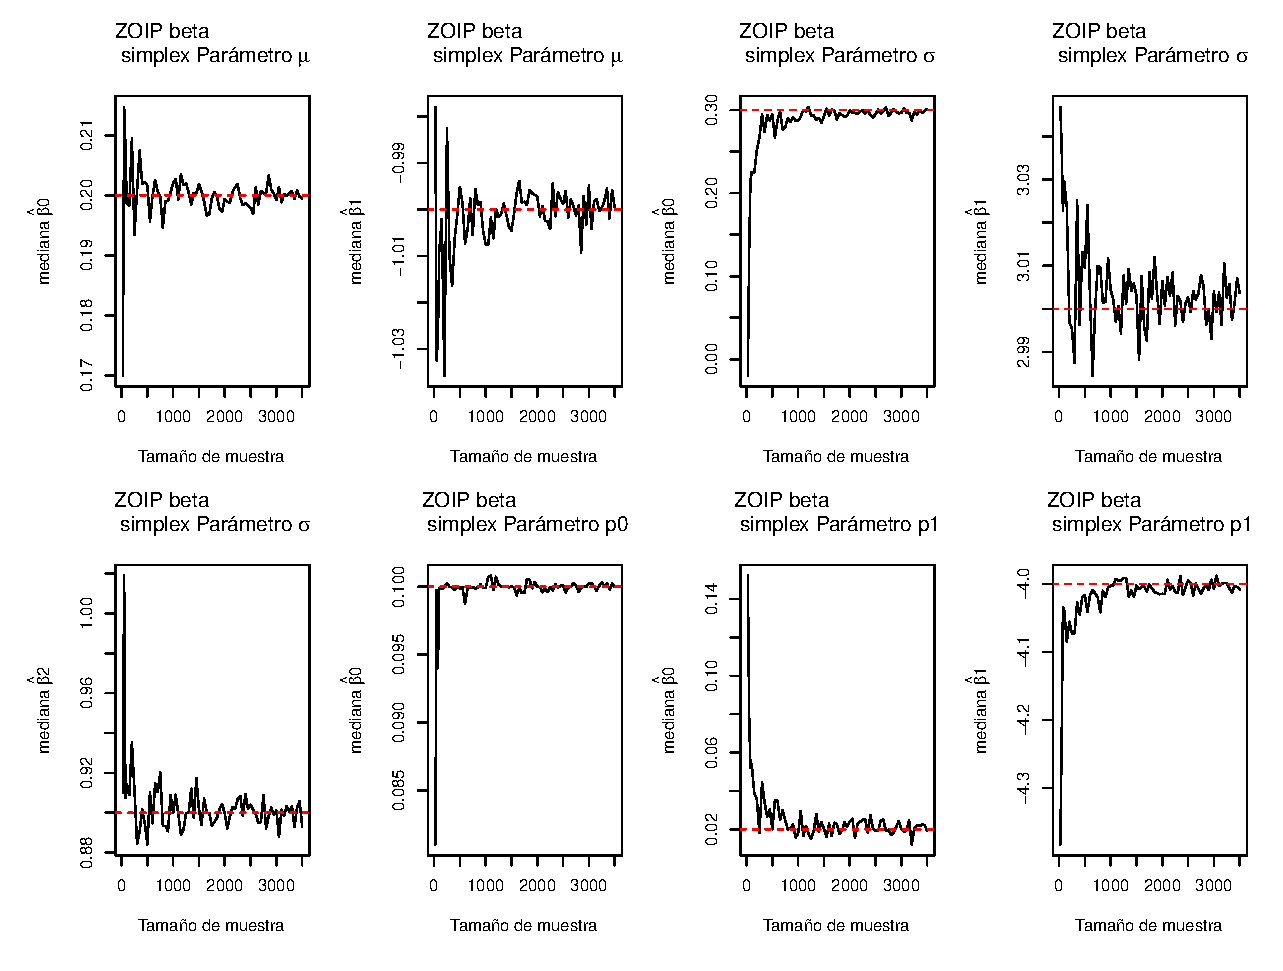
\includegraphics[scale=0.5]{Converg_Simplex.eps}	
		\caption{Simulaci\'{o}n de un modelo de regresi\'{o}n ZOIP-simplex con diferentes valores de $n$.}
		\label{Simu_simplex}
	\end{center}
\end{figure}

En la figura \ref{Simu_simplex} se describen los valores estimados para diferentes tama\~{n}os de muestra, cuando se elige realizar una regresi\'{o}n ZOIP-simplex, Se nota como todos los par\'{a}metros oscilan alrededor de los valores verdaderos y como estas oscilaciones se van reduciendo a trav\'{e}s de que el tama\~{n}o de muestra crece, sin embargo, unos par\'{a}metros toman mayor tiempo de convergencia como es el par\'{a}metro $\beta_1$ asociado al par\'{a}metro de dispersi\'{o}n ($\sigma$).\\



\begin{table}[!hbt]
{\scriptsize
\begin{center}
\begin{tabular}{|c|cc|ccc|c|cc|}\hline
\multirow{2}{*}{Familia} & \multicolumn{2}{|c|}{$\mu$} & \multicolumn{3}{|c|}{$\sigma$} & $p_0$ & \multicolumn{2}{|c|}{$p_1$} \\ \cline{2-9}
& $\hat{\beta}_0$& $\hat{\beta}_1$& $\hat{\beta}_0$& $\hat{\beta}_1$& $\hat{\beta}_2$& $\hat{\beta}_0$ & $\hat{\beta}_0$ & $\hat{\beta}_1$ \\ \hline \hline
R-S & 1.25 & 0.32 & 1.45 & 2.55 & 1.38 & 4.86 & 383.09 & 4.88 \\ 
F-C & 14.22 & 3.96 & 22.21 & 2.9 & 10.14 & 4.86 & 91.21 & 4.88 \\
original & 22.34 & 8.03 & 22.55 & 3.62 & 8.69 & 4.84 & 90.58 & 4.96 \\
simplex & 13.93 & 5.89 & 24.49 & 3.11 & 11.01 & 4.85 & 91.15 & 4.81 \\ \hline
\end{tabular}
\caption{Mediana del MAPE (Error porcentual absoluto medio) en porcentaje para los diferentes parametros en las diferentes parametrizaciones.}
\label{MAPE}
\end{center}
}
\end{table}

En la tabla \ref{MAPE} se muestra la mediana del MAPE de los diferentes par\'{a}metros regresores para cada posible caso de la distribuci\'{o}n o parametrizaci\'{o}n de la distribuci\'{o}n ZOIP, en dicha tabla se nota como el MAPE en los interceptos de cualquier regresi\'{o}n asociada a los par\'{a}metros de la distribuci\'{o}n ZOIP son un poco m\'{a}s grandes que los dem\'{a}s par\'{a}metros regresores de cada regresi\'{o}n, adem\'{a}s se comete un MAPE m\'{a}s grande en las regresiones asociadas a todos los par\'{a}metros de inflaci\'{o}n, esto nos permite concluir que hallar los par\'{a}metros verdaderos en los par\'{a}metros de inflaci\'{o}n es un poco m\'{a}s dif\'{\i}cil que en los par\'{a}metros de localizaci\'{o}n y escala como lo son $\mu$ y $\sigma$, esto se debe a que se posee una menor cantidad de datos en cero y uno, en este escenario de simulaci\'{o}n elegido. Por otro lado, el intercepto asociado a la regresi\'{o}n del par\'{a}metro de inflaci\'{o}n de los unos posee un MAPE muy grande, por lo que nos permite concluir que a pesar de que los diferentes par\'{a}metros estimados en la simulaci\'{o}n oscilan alrededor del valor real este todav\'{\i}a tiene una variabilidad muy grande por lo que hace que este MAPE sea grande y el par\'{a}metro no haya convergido con un tama\~{n}o de muestra de 3500.\\

\begin{figure}
	\begin{center}
		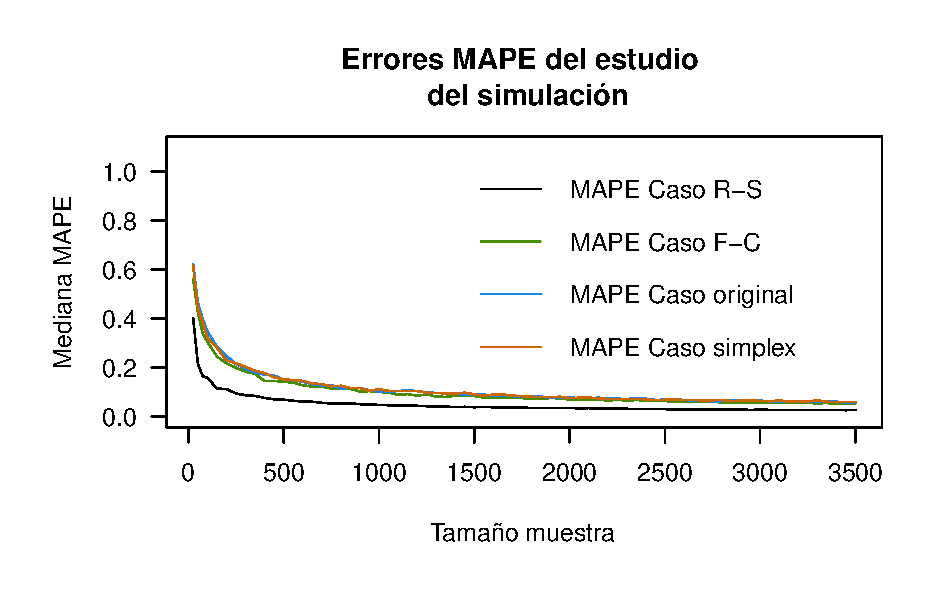
\includegraphics[scale=0.6]{MAPE_gnral.eps}	
		\caption{Mape (Error porcentual absoluto medio) para modelo de regresion ZOIP si\-mu\-la\-do para distintas parametrizaciones y valores de $n$.}
		\label{Mape_gnrl}
	\end{center}
\end{figure}

En la figura \ref{Mape_gnrl} se muestra la mediana del MAPE de la mediana del MAPE de todos los par\'{a}metros asociados a cada parametrizaci\'{o}n y distribuci\'{o}n para diferentes tama\~{n}os de muestra, en ella se evidencia como el caso de la regresi\'{o}n ZOIP-beta con parametrizaci\'{o}n \cite{Stasinopoulos2} tiene un MAPE menor, donde este tiene asociados unos par\'{a}metros distintos con una distribuci\'{o}n ZOIP con menor variabilidad, por lo que no es del todo comparable con las dem\'{a}s parametrizaciones y distribuciones, se nota un MAPE menor al $20\%$ a partir de un tama\~{n}o de muestra mayor a 500, por lo que se puede concluir que con un tama\~{n}o de muestra mayor a 500 el modelo tendr\'{a} un MAPE aceptable para la estimaci\'{o}n de todos los par\'{a}metros de la regresi\'{o}n ZOIP, sin embargo, esto siempre depender\'{a} de la variabilidad que posean los datos.

\subsection{Datos reales}

En una entidad financiera tiene gran importancia conocer el comportamiento del porcentaje de utilizaci\'{o}n de las tarjetas de cr\'{e}dito (tdc), con el fin de conocer el comportamiento de la cartera de tarjeta de cr\'{e}dito, adem\'{a}s de detectar los diferentes factores que pueden afectar este tipo de cartera. Se define a $y$ como el porcentaje de uso de una tdc, es de notar que $y$ se encuentra entre cero y uno, pero adicional es normal que se tengan tdc que no sean utilizadas ($y=0$) y tdc que est\'{a}n utilizadas en la totalidad de su cupo asignado ($y=1$), por lo que se trata a $y$ como una variable aleatoria perteneciente a datos proporcionales inflados con ceros y unos, es decir $y$ puede ser explicada a partir de una distribuci\'{o}n ZOIP. Se tiene un total de 9206 tarjetas de cr\'{e}dito. Se quiere estudiar el impacto de algunas variables sobre el porcentaje de utilizaci\'{o}n de una tdc, para ello se busca ajustar un modelo de regresi\'{o}n ZOIP mediante la funci\'{o}n \code{RM.ZOIP} del paquete \pkg{ZOIP} de \proglang{R}, que permita explicar el comportamiento del porcentaje de utilizaci\'{o}n de una tdc mediante las siguientes tres variables, \textsl{Score:} variable entre cero y 1000 que para nuestro caso se cambiara de escala entre cero y uno, est\'{a} explica la calificaci\'{o}n del comportamiento de pago del cliente asociada a la tdc, que pertenece a la entidad financiera, donde cero es la peor calificacion y uno un comportamiento de pago ideal; \textsl{Prom Cuotas:} se define como el promedio de cantidad de cuotas al que ha diferido sus compras en los \'{u}ltimos seis meses; \textsl{Cupo tdc Entidad:} es el cupo total asignado a la tdc, esta ser\'{a} tratada como el logaritmo de su cupo m\'{a}s uno, para una mayor estabilidad de su varianza.\\

En el modelo de regresi\'{o}n ZOIP se deben definir cuatro diferentes modelos de regresi\'{o}n para ser ajustados, de tal forma que nos permita ver el efecto de las variables descritas anteriormente sobre cada uno de los par\'{a}metros de la distribuci\'{o}n ZOIP, adicionalmente dependiendo de la parametrizaci\'{o}n o distribuci\'{o}n que se est\'{e} utilizando, se debe utilizar una funci\'{o}n enlace adecuada para cada regresi\'{o}n, en las ecuaciones dadas en \eqref{A_eq_reg} se pueden ver los modelos de regresi\'{o}n a aplicar en cada par\'{a}metro, en estas ecuaciones se ve que dependen de una funci\'{o}n enlace $h(\cdot)$, en la tabla \ref{T_F_enlace2} se muestran las diferentes funciones enlaces adecuadas para cada par\'{a}metro dependiendo de la distribuci\'{o}n escogida y/o la parametrizaci\'{o}n.\\

Si $y_{i} \sim ZOIP(\mu_{i},\sigma_{i},p_{0i}, p_{1i}),$

\begin{equation}
\begin{split}
&h_1(\mu_{i})=\beta_0+\beta_1 x_{1i}+\beta_2 x_{2i}+\beta_3 x_{3i},\\
&h_2(\sigma_{i})=\beta_0+\beta_1 x_{1i}+\beta_2 x_{2i}+\beta_3 x_{3i},\\
&h_3(p_{0i})=\beta_0+\beta_1 x_{1i}+\beta_2 x_{2i}+\beta_3 x_{3i},\\
&h_4(p_{1i}) =\beta_0+\beta_1 x_{1i}+\beta_2 x_{2i}+\beta_3 x_{3i},
\end{split}
\label{A_eq_reg}
\end{equation}

donde $y_i$ es porcentaje de utilizacion de la i-esima tdc, $x_{1i}$: es el valor del score del i-esimo individuo asociada a la tarjeta de cr\'{e}dito, $x_{2i}$: es valor del promedio de cuotas al que difiere sus compras de la i-esima tarjeta de cr\'{e}dito, $x_{3i}$: es el valor del cupo otorgado de la i-esima tarjeta de cr\'{e}dito. 

\begin{table}[!hbt]
{\scriptsize
\begin{center}
\begin{tabular}{|c|c|c|}\hline
Familia & Par\'{a}metro & $h(\cdot)$ \\ \hline
\multirow{4}{*}{R-S} & $\mu$ & Logit \\
 & $\sigma$ & Logit \\
 & $p_0$ & Logit \\
 & $p_1$ & Logit \\ \hline

\multirow{4}{*}{F-C} & $\mu$ & Logit \\
 & $\sigma$ & Log. \\
 & $p_0$ & Logit \\
 & $p_1$ & Logit \\ \hline

\multirow{4}{*}{original} & $\mu$ & Log. \\
 & $\sigma$ & Log. \\
 & $p_0$ & Logit \\
 & $p_1$ & Logit \\ \hline

\multirow{4}{*}{simplex} & $\mu$ & Logit \\
 & $\sigma$ & Log. \\
 & $p_0$ & Logit \\
 & $p_1$ & Logit \\ \hline

\end{tabular}
\caption{Funciones de enlace adecuadas para cada par\'{a}metro, seg\'{u}n su distribuci\'{o}n y/o parametrizaci\'{o}n para el modelo de regresi\'{o}n ZOIP en el porcentaje de utilizaci\'{o}n de una tdc.}
\label{T_F_enlace2}
\end{center}
}
\end{table}

En las ecuaciones dadas en \eqref{A_eq_reg} se puede ver como los par\'{a}metros $\mu$, $\sigma$, $p_0$, $p_1$ ser\'{a}n explicados por las variables score, cupo asignado a su tdc y el promedio al que difiere sus compras, bajo estas ecuaciones podemos observar como se explica el porcentaje utilizaci\'{o}n de una tdc, la variabilidad de este porcentaje de utilizaci\'{o}n, el por que un cliente no llega a utilizar nunca su tdc y adicional y contrariamente a lo anterior, por que un cliente utiliza la total capacidad de su tdc.\\

\begin{table}[!hbt]
{\scriptsize
\begin{center}
\begin{tabular}{|c|c|c|ccc|c|c|}\hline
Familia & Par\'{a}metro & $\beta$'s & Estimaci\'{o}n & Error est\'{a}ndar & Valor P & Log-Verosimilitud & Iteraciones \\ \hline \hline
\multirow{12}{*}{R-S} & \multirow{4}{*}{$\mu$} & $\hat{\beta}_0$ & -0.046	&0.050	&0.3618 & \multirow{12}{*}{-5414.738} & \multirow{12}{*}{125}  \\
& & $\hat{\beta}_1$ & -0.354	&0.107	&0.0009 & &\\
& & $\hat{\beta}_2$ & 0.022	&0.002	&$<2.2e^{-16}$ & & \\
& & $\hat{\beta}_3$ & -0.025	&0.009	&0.0074 & & \\ \cline{2-6}
& \multirow{4}{*}{$\sigma$} & $\hat{\beta}_0$ & 0.822	&0.038	&$<2.2e^{-16}$  & &\\
& & $\hat{\beta}_1$ & -0.197	&0.078	&0.0114  & &\\
& & $\hat{\beta}_2$ & -0.006	&0.002	&0.0013  & &\\
& & $\hat{\beta}_3$ & -0.003	&0.007	&0.6741  & &\\ \cline{2-6}
& \multirow{4}{*}{$p_0$} & $\hat{\beta}_0$ & -1.496	&0.101	&$<2.2e^{-16}$  & &\\
& & $\hat{\beta}_1$ & 0.724	&0.185	&$8.87e^{-5}$  & &\\
& & $\hat{\beta}_2$ & -0.153	&0.009	&$<2.2e^{-16}$  & &\\
& & $\hat{\beta}_3$ & 0.002	&0.015	&0.1243  & &\\ \cline{2-6}
& \multirow{4}{*}{$p_1$} & $\hat{\beta}_0$ &-1.480	&0.095	&$<2.2e^{-16}$  & &\\
& & $\hat{\beta}_1$ & -0.630	&0.254	&0.0132  & &\\
& & $\hat{\beta}_2$ & 0.011	&0.006	&0.0666  & &\\
& & $\hat{\beta}_3$ & -0.069	&0.022	&0.0022  & &\\ \hline

\end{tabular}
\caption{Parametros regresores estimados de un modelo de regresi\'{o}n ZOIP-beta con parametrizaci\'{o}n Rigby y Stasinopoulos (2005) en el porcentaje de utilizaci\'{o}n de una tdc.}
\label{T_Apli_CC_RS}
\end{center}
}
\end{table}


\begin{table}[!hbt]
{\scriptsize
\begin{center}
\begin{tabular}{|c|c|c|ccc|c|c|}\hline
Familia & Par\'{a}metro & $\beta$'s & Estimaci\'{o}n & Error est\'{a}ndar & Valor P & Log-Verosimilitud & Iteraciones \\ \hline \hline
\multirow{12}{*}{F-C} & \multirow{4}{*}{$\mu$} & $\hat{\beta}_0$ & -0.045	&0.050	&0.3667  & \multirow{12}{*}{-5414.605} & \multirow{12}{*}{105} \\
& & $\hat{\beta}_1$ & -0.354	&0.107	&0.0009   & &\\
& & $\hat{\beta}_2$ & 0.022	&0.002	&$<2.2e^{-16}$   & &\\
& & $\hat{\beta}_3$ & -0.025	&0.009	&0.0074   & &\\ \cline{2-6}
& \multirow{4}{*}{$\sigma$} & $\hat{\beta}_0$ & 0.068	&0.045	&0.1286   & &\\
& & $\hat{\beta}_1$ & 0.238	&0.094	&0.0117   & &\\
& & $\hat{\beta}_2$ & 0.007	&0.002	&0.0012   & &\\
& & $\hat{\beta}_3$ & 0.003	&0.008	&0.6854   & &\\ \cline{2-6}
& \multirow{4}{*}{$p_0$} & $\hat{\beta}_0$ & -1.496	&0.101	&$<2.2e^{-16}$  & &\\
& & $\hat{\beta}_1$ & 0.724	&0.185	&$8.87e^{-5}$  & &\\
& & $\hat{\beta}_2$ & -0.153	&0.009	&$<2.2e^{-16}$  & &\\
& & $\hat{\beta}_3$ & 0.002	&0.015	&0.1243  & &\\ \cline{2-6}
& \multirow{4}{*}{$p_1$} & $\hat{\beta}_0$ &-1.480	&0.095	&$<2.2e^{-16}$  & &\\
& & $\hat{\beta}_1$ & -0.630	&0.254	&0.0132  & &\\
& & $\hat{\beta}_2$ & 0.011	&0.006	&0.0666  & &\\
& & $\hat{\beta}_3$ & -0.069	&0.022	&0.0022  & &\\ \hline

\end{tabular}
\caption{Parametros regresores estimados de un modelo de regresi\'{o}n ZOIP-beta con parametrizaci\'{o}n Ferrari y Cribari-Neto (2004) en el porcentaje de utilizaci\'{o}n de una tdc.}
\label{T_Apli_CC_FC}
\end{center}
}
\end{table}


\begin{table}[!hbt]
{\scriptsize
\begin{center}
\begin{tabular}{|c|c|c|ccc|c|c|}\hline
Familia & Par\'{a}metro & $\beta$'s & Estimaci\'{o}n & Error est\'{a}ndar & Valor P & Log-Verosimilitud & Iteraciones \\ \hline \hline
\multirow{12}{*}{original} & \multirow{4}{*}{$\mu$} & $\hat{\beta}_0$ & -0.649	&0.048	&$<2.2e^{-16}$  & \multirow{12}{*}{-5415.386} & \multirow{12}{*}{121} \\
& & $\hat{\beta}_1$ & 0.035	&0.103	&0.7311   & &\\
& & $\hat{\beta}_2$ & 0.019	&0.002	&$<2.2e^{-16}$   & &\\
& & $\hat{\beta}_3$ & -0.011	&0.009	&0.2267 & & \\ \cline{2-6}
& \multirow{4}{*}{$\sigma$} & $\hat{\beta}_0$ & -0.611	&0.054	&$<2.2e^{-16}$   & &\\
& & $\hat{\beta}_1$ & 0.397	&0.111	&0.0003   & &\\
& & $\hat{\beta}_2$ & -0.002	&0.003	&0.4724   & &\\
& & $\hat{\beta}_3$ & 0.015	&0.010	&0.1456   & &\\ \cline{2-6}
& \multirow{4}{*}{$p_0$} & $\hat{\beta}_0$ & -1.496	&0.101	&$<2.2e^{-16}$  & &\\
& & $\hat{\beta}_1$ & 0.724	&0.185	&$8.87e^{-5}$  & &\\
& & $\hat{\beta}_2$ & -0.153	&0.009	&$<2.2e^{-16}$  & &\\
& & $\hat{\beta}_3$ & 0.002	&0.015	&0.1243  & &\\ \cline{2-6}
& \multirow{4}{*}{$p_1$} & $\hat{\beta}_0$ &-1.480	&0.095	&$<2.2e^{-16}$  & &\\
& & $\hat{\beta}_1$ & -0.630	&0.254	&0.0132  & &\\
& & $\hat{\beta}_2$ & 0.011	&0.006	&0.0666  & &\\
& & $\hat{\beta}_3$ & -0.069	&0.022	&0.0022  & &\\ \hline


\end{tabular}
\caption{Parametros regresores estimados de un modelo de regresi\'{o}n ZOIP-beta con parametrizaci\'{o}n original en el porcentaje de utilizaci\'{o}n de una tdc.}
\label{T_Apli_CC_Ori}
\end{center}
}
\end{table}


\begin{table}[!hbt]
{\scriptsize
\begin{center}
\begin{tabular}{|c|c|c|ccc|c|c|}\hline
Familia & Par\'{a}metro & $\beta$'s & Estimaci\'{o}n & Error est\'{a}ndar & Valor P & Log-Verosimilitud & Iteraciones \\ \hline \hline
\multirow{12}{*}{simplex} & \multirow{4}{*}{$\mu$} & $\hat{\beta}_0$ & 0.180	&0.050	&0.0003  & \multirow{12}{*}{-22385.78} & \multirow{12}{*}{117} \\
& & $\hat{\beta}_1$ & -3.890	&0.206	&$<2.2e^{-16}$   & &\\
& & $\hat{\beta}_2$ & 0.166	&0.004	&$<2.2e^{-16}$   & &\\
& & $\hat{\beta}_3$ & -0.128	&0.019	&$5.85e^{-12}$   & &\\ \cline{2-6}
& \multirow{4}{*}{$\sigma$} & $\hat{\beta}_0$ & 11.59	&0.062	&$<2.2e^{-16}$   & &\\
& & $\hat{\beta}_1$ & 0.063	&0.240	&0.7918   & &\\
& & $\hat{\beta}_2$ & 0.134	&0.004	&$<2.2e^{-16}$  & &\\
& & $\hat{\beta}_3$ & 0.344	&0.023	&$<2.2e^{-16}$   & &\\ \cline{2-6}
& \multirow{4}{*}{$p_0$} & $\hat{\beta}_0$ & -1.496	&0.101	&$<2.2e^{-16}$  & &\\
& & $\hat{\beta}_1$ & 0.724	&0.185	&$8.87e^{-5}$  & &\\
& & $\hat{\beta}_2$ & -0.153	&0.009	&$<2.2e^{-16}$  & &\\
& & $\hat{\beta}_3$ & 0.002	&0.015	&0.1243  & &\\ \cline{2-6}
& \multirow{4}{*}{$p_1$} & $\hat{\beta}_0$ &-1.480	&0.095	&$<2.2e^{-16}$  & &\\
& & $\hat{\beta}_1$ & -0.630	&0.254	&0.0132  & &\\
& & $\hat{\beta}_2$ & 0.011	&0.006	&0.0666  & &\\
& & $\hat{\beta}_3$ & -0.069	&0.022	&0.0022  & &\\ \hline

\end{tabular}
\caption{Parametros regresores estimados de un modelo de regresi\'{o}n ZOIP-simplex en el porcentaje de utilizaci\'{o}n de una tdc.}
\label{T_Apli_CC_Sim}
\end{center}
}
\end{table}

En las tablas \ref{T_Apli_CC_RS}, \ref{T_Apli_CC_FC}, \ref{T_Apli_CC_Ori}, \ref{T_Apli_CC_Sim} se tiene informaci\'{o}n sobre como las covariables influyen en los par\'{a}metros de los cuatro diferentes modelos ajustados de la regresi\'{o}n ZOIP, primero se puede ver que al modelar el par\'{a}metro de la media, es decir, el porcentaje medio de utilizaci\'{o}n de la tdc, la variable regresora score afecta de manera negativa y significativa en cada uno de los modelos ajustados, excepto en el mo\-de\-lo con parametrizaci\'{o}n original, en el cual el par\'{a}metro no dio significativo, esto nos indica que a un mejor comportamiento de pago, menos utilizaci\'{o}n de la tdc, sobre el par\'{a}metro del promedio de cuotas diferidas vemos como el par\'{a}metro $\beta_2$ sin excepci\'{o}n alguna en todos los modelos es la variable m\'{a}s significativa que permite explicar la proporci\'{o}n media de la utilizaci\'{o}n de una tdc, esto nos indica que a medida que los clientes difieren a mayores cuotas sus compras con la tdc estar\'{a}n utilizando m\'{a}s su tdc, algo muy l\'{o}gico, desde el punto de vista del problema; ahora el par\'{a}metro $\beta_3$ asociado al cupo de su tdc tiene un efecto negativo aunque no muy significativo sobre la variable respuesta, lo cual indicar\'{\i}a que a mayor cupo en su tdc un poco menos de utilizaci\'{o}n de la tdc estar\'{a} acompa\~{n}ado.\\

Al analizar el efecto de la variabilidad de la utilizaci\'{o}n de las tdc, se observa como el par\'{a}metro de score tiene un efecto positivo sobre la precisi\'{o}n de la utilizaci\'{o}n de la tdc, en el modelo ZOIP-beta parametrizaci\'{o}n \cite{Stasinopoulos2} este efecto parece ser negativo, pero $\sigma$ al estar representando la dispersi\'{o}n y no la precisi\'{o}n, estar\'{\i}a dando un efecto positivo sobre la precisi\'{o}n, por lo tanto a mejor comportamiento de pago la utilizaci\'{o}n de la tdc ser\'{a}n m\'{a}s parecidas entre los individuos, cabe resaltar que $\beta_1$ no es significativo en el modelo simplex. Adem\'{a}s el par\'{a}metro $\beta_3$ asociado al cupo de la tdc no influye sobre la variabilidad en ninguno de los modelos propuestos, excepto en modelo de regresi\'{o}n ZOIP-simplex que tiene un efecto positivo sobre la variabilidad de los porcentajes de utilizaci\'{o}n de las tdc.\\

Por otra parte el efecto de que alguien no utilice su tdc es exactamente igual en los cuatro modelos propuestos, esto por la metodolog\'{\i}a de estimaci\'{o}n de m\'{a}xima verosimilitud, y se puede observar como el comportamiento de pago y la cantidad de cuotas a las que se difiere las compras el cliente afectan de manera significativa la no utilizaci\'{o}n de las tdc. Adem\'{a}s es de resaltar que si los clientes no difieren a grandes cuotas sus compras y su comportamiento de pago es muy bueno estos clientes tendr\'{a}n mayor probabilidad de no utilizar para nada las tdc.\\

En el porcentaje de utilizaci\'{o}n global de la tdc, vemos como las tres covariables incluidas en el modelo afectan de manera significativa la utilizaci\'{o}n por completo de la tdc y vemos como la variable que es m\'{a}s significativa es el cupo de las tdc y que este tiene un efecto negativo sobre la probabilidad de utilizar por completo mi tdc, lo que me indica que a mayor cupo menor probabilidad de utilizar por completo de mi tdc (efecto que hab\'{\i}amos evidenciado en la explicaci\'{o}n de la utilizaci\'{o}n media de las tdc), el mismo efecto pasa sobre la variable score que me indica que a peor comportamiento de pago m\'{a}s utilizaci\'{o}n la tdc, sin embargo, si el cliente difiere a grandes cuotas su compras este tendera a tener una mayor probabilidad de utilizar por completo su tdc. cabe resaltar que el efecto de las covariables sobre la probabilidad de utilizar por completo la tdc es totalmente contrario al efecto causado sobre la probabilidad de no utilizar para nada la tdc, algo l\'{o}gico y esperado.\\

Al analizar el valor de la log-verosimilitud se observa que el mejor modelo de regresi\'{o}n que explica el porcentaje de utilizaci\'{o}n de una tdc en esta entidad financiera es la regresi\'{o}n ZOIP-beta, ya que posee un valor de log-verosimilitud menor que el modelo de regresi\'{o}n ZOIP-simplex, sin embargo, no importa la parametrizaci\'{o}n que se tenga en la regresi\'{o}n ZOIP-beta, porque el valor de la log-verosimilitud son significativamente iguales, sin embargo, el modelo que requiere menor n\'{u}mero de iteraciones para ser ajustado es la regresi\'{o}n ZOIP-beta parametrizaci\'{o}n \cite{Ferrari2} seguido por la parametrizaci\'{o}n original y por \'{u}ltimo la parametrizacion de \cite{Stasinopoulos2}.


%%%%%%%%%%%%%%%%%%%%%%%%%%%%%%%%%%%%%%%%%%%%%%%%%%%%%%%%%%%%%%%%%%%%%%%%%%%%%%%%%%%%%%%%%%%%%%%%%%%%%%%%%%%%%%%%%%%%%%%%%%%%%%%%%%%%%%%%%%%%%%%%%%%%%%%%%%%%%%%%%%

\section{Conclusi\'{o}n}

El modelo de regresi\'{o}n ZOIP, es un modelo de regresi\'{o}n de efectos fijos que es desarrollado bajo la distribuci\'{o}n ZOIP y el cual se encarga de encontrar las covariables o factores que m\'{a}s influyen en una variable respuesta cuya distribuci\'{o}n asociada es una distribuci\'{o}n ZOIP. La estimaci\'{o}n del efecto de las covariables sobre la variable respuesta se realiza mediante m\'{a}xima verosimilitud, dicha maximizaci\'{o}n de la verosimilitud no tiene una soluci\'{o}n cerrada anal\'{\i}ticamente, por lo que se realiza computacionalmente y el paquete \pkg{ZOIP} de \proglang{R} da una soluci\'{o}n a esto. Seg\'{u}n los estudios de simulaci\'{o}n realizados en este trabajo, las estimaciones convergen con un tama\~{n}o de muestra moderado a sus valores reales; aunque en ocasiones ocurre que las convergencias de los efectos de las covariables asociadas a los par\'{a}metros de inflaci\'{o}n requieren un mayor n\'{u}mero de muestras para demostrar su convergencia.\\

En el modelo de regresi\'{o}n ZOIP y el paquete \pkg{ZOIP} de \proglang{R} es posible realizar de una ma\-ne\-ra muy sencilla los principales tipos de regresiones para datos proporciones inflados con ceros y unos que existen, como la regresi\'{o}n simplex y la regresi\'{o}n beta bajo diferentes parametrizaciones, adem\'{a}s el modelo de regresi\'{o}n ZOIP permite realizar ajustes a modelos inflados unilateralmente, es decir, donde solo haya datos proporcionales con valores cero o uno, e incluso realizar un ajuste sobre un modelo de regresi\'{o}n para datos proporcionales sin inflaciones.


\chapter{Cap\'{\i}tulo 4: Modelo de regresi\'{o}n ZOIP con efectos mixtos}\label{cap4}
%{\Huge \textbf{Modelo de regresi\'{o}n ZOIP con efectos mixtos\\}}

Los modelos de regresi\'{o}n mixtos han sido de mucho inter\'{e}s en la \'{u}ltima \'{e}poca, por su capacidad de estimar el efecto de una variable sobre el modelo, a trav\'{e}s de la estimaci\'{o}n de la varianza de la distribuci\'{o}n de la variable, estos fueron introducidos de una manera general por \cite{Laird1}. Es por esto que los modelos de regresi\'{o}n mixtos tambi\'{e}n han sido implementados cuando la variable respuesta es tomada por una variable aleatoria perteneciente a datos proporcionales, tal es el caso de \cite{Stasinopoulos2} en los modelos aditivos generalizados para localizaci\'{o}n, escala y forma (Gamlss) que implementan el modelo de regresi\'{o}n beta con intercepto aleatorio normal, as\'{\i} otros autores como \cite{Verkuilen1} y \cite{Bonat1} proponen modelos de regresi\'{o}n beta con efectos aleatorios normales, estimados a partir de m\'{a}xima verosimilitud marginal y metodolog\'{\i}as bayesianas. \cite{Figueroa1} extienden el modelo propuesto por \cite{Ferrari2} a un modelo con efectos fijos y aleatorios bajo la distribuci\'{o}n normal y bajo la distribuci\'{o}n t en estructuras de regresi\'{o}n tanto para el par\'{a}metro de la media, como del par\'{a}metro de precisi\'{o}n, la estimaci\'{o}n de los par\'{a}metros del modelo de regresi\'{o}n fue realizado bajo una perspectiva bayesiana, mediante implementaciones computacionales del muestreador de Gibbs. \cite{Usuga1} desarrollan el modelo de regresi\'{o}n beta mixto para datos proporcionales longitudinales, bajo intercepto y pendiente aleatoria normal y no normal, la estimaci\'{o}n de los par\'{a}metros es realizada v\'{\i}a m\'{a}xima verosimilitud y la cuadratura de Gauss-Hermite adaptativa. Otros autores como \cite{Song1} implementan un modelo de regresi\'{o}n mixto para una variable respuesta bajo la distribuci\'{o}n simplex, \cite{Bonat2} tambi\'{e}n realiza un an\'{a}lisis de verosimilitud del modelo beta mixto, donde la estimaci\'{o}n de los par\'{a}metros de regresi\'{o}n es realizada bajo algoritmos MCMC.\\

Como se pudo notar anteriormente, se ve que las metodolog\'{\i}as de estimaci\'{o}n de los pa\-r\'{a}\-me\-tros del modelo de regresi\'{o}n mixto no tienen una soluci\'{o}n cerrada anal\'{\i}ticamente y es un poco m\'{a}s complicada cuando se trata de una variable respuesta perteneciente a datos proporcionales, por lo que se utilizan ciertas aproximaciones o en la mayor\'{\i}a de los casos metodolog\'{\i}as y algoritmos bayesianos para la estimaci\'{o}n de los par\'{a}metros regresores. Una de las metodolog\'{\i}as utilizadas es la aproximaci\'{o}n de la funci\'{o}n de verosimilitud v\'{\i}a la cuadratura de Gauss-Hermite adaptativa, utilizada e implementada en los modelos de regresi\'{o}n beta mixtos por \cite{Usuga1} y es utilizada para la estimaci\'{o}n del modelo de regresi\'{o}n ZOIP mixto, dicha cuadratura fue implementada anteriormente por \cite{Fahrmeir1} sobre los modelos lineales generalizados. Diversos estudios para la estimaci\'{o}n de par\'{a}metros sobre modelos estad\'{\i}sticos han sido implementados mediante esta t\'{e}cnica, por ejemplo, el trabajo realizado por \cite{Liu1} y \cite{Smithson1} que estima los par\'{a}metros del modelo de regresi\'{o}n beta bajo la cuadratura de Gauss-Hermite. Por otra parte, se han realizado diversas modificaciones sobre la cuadratura de Gauss-Hermite original, tales como la cuadratura de Gauss-Hermite adaptativa y algunas mejoras sobre esta como la cuadratura de Gauss-Hermite adaptativa con \textit{pruning} \citep{Hernandez1}.\\

Los modelos de regresi\'{o}n mixtos que se han mencionado anteriormente sobre datos proporcionales, no se encuentran con presencia de datos en cero y/o uno, es decir inflados con ceros y/o unos, por lo que otros autores como \cite{Ospina2} presentaron una distribuci\'{o}n beta inflada con ceros o con unos, mediante una combinaci\'{o}n de una distribuci\'{o}n discreta y una distribuci\'{o}n continua dada por la distribuci\'{o}n beta con parametrizaci\'{o}n de \cite{Ferrari2} y la cual dio pie para que m\'{a}s adelante \cite{Ospina1} propusieran una clase general de modelos de regresi\'{o}n beta inflados en cero y uno. Recientemente \cite{Kosmidis1} han estudiado los modelos de regresi\'{o}n inflados para datos proporcionales, pero basados en una distribuci\'{o}n distinta a la propuesta por \cite{Ospina1}, sin embargo, cabe aclarar que los anteriores modelos son modelos de regresi\'{o}n para efectos fijos, es decir, no incluyen alg\'{u}n efecto aleatorio, por lo que otros autores como \cite{Galvis1} incluyen efectos aleatorios dentro de los modelos de regresi\'{o}n inflados con ceros y/o unos, basados en la distribuci\'{o}n propuesta por \cite{Ospina2}y otras distribuciones para datos proporcionales, como la distribuci\'{o}n simplex y beta-rectangular, la estimaci\'{o}n de los par\'{a}metros de regresi\'{o}n se realiz\'{o} mediante metodolog\'{\i}as bayesianas, MCMC.\\

Este cap\'{\i}tulo se encuentra organizado de la siguiente manera: primero se presenta el modelo de regresi\'{o}n ZOIP mixto basado en la distribuci\'{o}n ZOIP visto en el cap\'{\i}tulo \ref{cap2} y su debida estimaci\'{o}n, mediante m\'{a}xima verosimilitud, se muestra los diferentes tipos de cuadratura de Gauss-Hermite, para que posteriormente se muestre la aproximaci\'{o}n de la funci\'{o}n de verosimilitud v\'{\i}a la cuadratura de Gauss-Hermite adaptativa multidimensional, en la si\-gui\-en\-te secci\'{o}n se presenta la implementaci\'{o}n del modelo de regresi\'{o}n ZOIP mixto en el paquete \pkg{ZOIP} de \proglang{R} y por \'{u}ltimo se presenta unas aplicaciones a datos simulados y a datos reales.


%%%%%%%%%%%%%%%%%%%%%%%%%%%%%%%%%%%%%%%%%%%%%%%%%%%%%%%%%%%%%%%%%%%%%%%%%%%%%%%%%%%%%%%%%%%%%%%%%%%%%%%%%%%%%%%%%%%%%%%%%%%%%%%%%%%%%%%%%%%%%%%%%%%%%%%%%%%%%%%%%%

\section{Modelo de regresi\'{o}n ZOIP mixto}


%Una estructura jer\'{a}rquica de dos niveles considerada para un modelo con variable respuesta dada por la distribuci\'{o}n para datos proporcionales inflados con ceros y/o unos (ZOIP), vista en la secci\'{o}n \ref{Sec_dist_zoip}. 

Sea $y_{ij}$ la $j-$\'{e}sima medida del $i-$\'{e}simo grupo, una escritura matem\'{a}tica para el modelo es la siguiente:


%las cantidades si asumisos interceptos aleatorios $\gamma_{1i}$ y $\gamma_{2i}$, los cuales son independientes y cada uno sigue una distribuci\'{o}n normal con media cero y desviaci\'{o}n est\'{a}ndar $\lambda_1$ y $\lambda_2$, respectivamente. Asumimos tambi\'{e}n que los interceptos aleatorios $\gamma_{1i}$ y $\gamma_{2i}$ son independientes entre s\'{\i}.

\begin{align}
\begin{split}
y_{ij}| \gamma_{1i},\gamma_{2i} & \overset{\text{ind}}{\sim} ZOIP(\mu_{ij},\sigma_{ij},p_{0ij}, p_{1ij}),\\
	h_1(\mu_{ij}) &= \mathbf{x}_{ij1}^{\top} \boldsymbol{\beta}_1+ \gamma_{1i},\\
	h_2(\sigma_{ij}) &= \mathbf{x}_{ij2}^{\top} \boldsymbol{\beta}_2+ \gamma_{2i},\\
	h_3(p_{0ij}) &= \mathbf{x}_{ij3}^{\top} \boldsymbol{\beta}_3,\\
	h_4(p_{1ij}) &= \mathbf{x}_{ij4}^{\top} \boldsymbol{\beta}_4,\\
	\gamma_{1i} & \overset{\text{i.i.d}}{\sim}  N(0,\lambda_1^2),\\
	\gamma_{2i} & \overset{\text{i.i.d}}{\sim}  N(0,\lambda_2^2),
\end{split}
\label{Mod_pmix}
\end{align}

%\[
%y_{ij}| \gamma_{1i},\gamma_{2i} \overset{\text{ind}}{\sim} ZOIP(\mu_{ij},\sigma_{ij},p_{0ij}, p_{1ij}),
%\]
%\[
%\gamma_{1i} \overset{\text{i.i.d}}{\sim}  N(0,\lambda_1^2),
%\]
%\[
%\gamma_{2i} \overset{\text{i.i.d}}{\sim}  N(0,\lambda_2^2),
%\]
%\\

con $i=1,2,\ldots, N$ y $j=1,2,\ldots, n_i$. Los par\'{a}metros $\mu$, $\sigma$, $p_0$, $p_1$ son modelados en funci\'{o}n de un conjunto de covariables tales que los $\mathbf{x}_{ij1}$, $\mathbf{x}_{ij2}$, $\mathbf{x}_{ij3}$ y $\mathbf{x}_{ij4}$, son vectores de covariables conocidos de dimensi\'{o}n $k_1$, $k_2$, $k_3$ y $k_4$ respectivamente. Los $\boldsymbol{\beta}_1$, $\boldsymbol{\beta}_2$, $\boldsymbol{\beta}_3$ y $\boldsymbol{\beta}_4$ son vectores de par\'{a}metros desconocidos fijos asociados a las covariables y $\gamma_{1i}$, $\gamma_{2i}$ son los interceptos aleatorios asociados al $i-$\'{e}simo grupo y cada uno distribuido normal con media cero y desviaci\'{o}n est\'{a}ndar $\lambda_1$ y $\lambda_2$, respectivamente, llamados componentes de varianza, asumimos tambi\'{e}n que los interceptos aleatorios $\gamma_{1i}$ y $\gamma_{2i}$ son independientes entre s\'{\i}. Adem\'{a}s las funciones $h_1(\cdot)$, $h_2(\cdot)$, $h_3(\cdot)$ y $h_4(\cdot)$ son funciones de enlace conocidas y apropiadas para mapear de los reales a los valores admisibles del par\'{a}metro, adem\'{a}s son funciones estrictamente mon\'{o}tonas y doblemente diferenciables. Las posibles funciones para el par\'{a}metro $\mu$ y $\sigma$ son logit, probit, clog-log, o log dependiendo de la parametrizaci\'{o}n usada, para los par\'{a}metros de inflaci\'{o}n $p_0$ y $p_1$ son posibles funciones de enlace como logit, probit, clog-log.

% Los par\'{a}metros $\mu$, $\sigma$, $p_0$ y $p_1$ son modelados linealmente en funci\'{o}n de un conjunto de covariables respectivamente, por:


%\[
%h_1(\mu_{ij})=\mathbf{x}_{ij1}^{\top} \boldsymbol{\beta}_1+ \gamma_{1i},
%\]
%\[
%h_2(\sigma_{ij})=\mathbf{x}_{ij2}^{\top} \boldsymbol{\beta}_2+ \gamma_{2i},
%\]
%\[
%h_3(p_{0ij})=\mathbf{x}_{ij3}^{\top} \boldsymbol{\beta}_3,
%\]
%\[
%h_4(p_{1ij})=\mathbf{x}_{ij4}^{\top} \boldsymbol{\beta}_4
%\] 

\subsection{Inferencia estad\'{\i}stica}

Para la estimaci\'{o}n de los par\'{a}metros del modelo de regresi\'{o}n dado por la expresi\'{o}n \eqref{Mod_pmix}, por medio de m\'{a}xima verosimilitud, es necesario definir el vector de par\'{a}metros y la funci\'{o}n de verosimilitud.

El vector de par\'{a}metros para el modelo \eqref{Mod_pmix} es $\boldsymbol{\theta}=(\boldsymbol{\beta_1}^{\top},\boldsymbol{\beta_2}^{\top},\boldsymbol{\beta_3}^{\top}, \boldsymbol{\beta_4}^{\top},\lambda_1,\lambda_2)^{\top}$ y pertenece al espacio:
\[
\Theta=\left\{\boldsymbol{\theta} \in \mathbb{R}^k | \boldsymbol{\beta_1} \in \mathbb{R}^{k_1}, \boldsymbol{\beta_2} \in \mathbb{R}^{k_2}, \boldsymbol{\beta_3} \in \mathbb{R}^{k_3}, \boldsymbol{\beta_4} \in \mathbb{R}^{k_4}, \lambda_1 \in \mathbb{R}^+, \lambda_2 \in \mathbb{R}^+  \right\},
\]

en el que $k=k_1+k_2+k_3+k_4+2$. La distribuci\'{o}n marginal de $\mathbf{y}_i=(y_{1i},\ldots, y_{n_i}i)^{\top}$ es dada por:

\[
f_y(\mathbf{y}_i;\boldsymbol{\theta})=\int_{\mathbb{R}^2}\prod_{j=1}^{n_i}f(y_{ij}|\gamma_{1i},\gamma_{2i})\cdot f(\gamma_{1i}|\lambda_1) f(\gamma_{2i}|\lambda_2) d\gamma_{1i}d\gamma_{2i},
\]

Entonces la funci\'{o}n de verosimilitud $L(\boldsymbol{\theta})$:



\begin{align*}
L(\boldsymbol{\theta}) &= \prod_{i=1}^{N}f_y(\mathbf{y}_i;\boldsymbol{\theta})\\
&= \prod_{i=1}^{N}\int_{\mathbb{R}^2}\prod_{j=1}^{n_i}f_y(y_{ij}|\gamma_{1i},\gamma_{2i})\cdot f(\gamma_{1i}|\lambda_1) f(\gamma_{2i}|\lambda_2) d\gamma_{1i}d\gamma_{2i},
\end{align*}

As\'{\i} la funci\'{o}n de log-verosimilitud $\ell(\boldsymbol{\theta})$ esta dado por:

\begin{equation}
\ell(\boldsymbol{\theta})=\sum_{i=1}^{N}log \left[\int_{\mathbb{R}^2}\prod_{j=1}^{n_i}f_y(y_{ij}|\gamma_{1i},\gamma_{2i})\cdot f(\gamma_{1i}|\lambda_1) f(\gamma_{2i}|\lambda_2) d\gamma_{1i}d\gamma_{2i}\right],
 \label{func_ver_mix}
\end{equation}


donde $f(y_{ij}|\gamma_{1i},\gamma_{2i})$ es la funci\'{o}n de densidad de probabilidad ZOIP y $f(\gamma_{1i}|\lambda_1)$ y $f(\gamma_{2i}|\lambda_2)$ son funciones de densidades de probabilidad normales con desviaciones est\'{a}ndar $\lambda_1$ y $\lambda_2$, respectivamente.\\

Para encontrar el $\boldsymbol{\theta}$ que maximiza la funci\'{o}n $\ell(\boldsymbol{\theta})$ es necesario solucionar la integral $N$ veces en $\mathbb{R}^2$, sin embargo esta integral no tiene forma cerrada, por lo que es necesario utilizar t\'{e}cnicas computacionales para la soluci\'{o}n de esta, t\'{e}cnicas tales como aproximaciones de Laplace, algoritmos EM, integraci\'{o}n Monte Carlo o t\'{e}cnicas bayesianas. Para solucionar dicha funci\'{o}n de log-verosimilitud en seste trabajo, se utiliz\'{o} el m\'{e}todo de integraci\'{o}n num\'{e}rica Gauss-Hermite adaptativa multidimensional con y sin \textit{pruning}, tal como se describe en la siguiente secci\'{o}n.


\subsection{Cuadratura de Gauss-Hermite}\label{sec:Cuadratura}

\subsubsection{Cuadratura de Gauss-Hermite unidimensional}

La cuadratura de Gauss-Hermite (GQ) es una herramienta \'{u}til para aproximar una integral de una funci\'{o}n $g(x)$ sobre $\Re$ con una suma ponderada, donde la variable $x$ es reemplazada por una cuadratura de $n$ puntos o nodos. Cada punto de la cuadratura es denotado por $p_i$, es evaluado en la funci\'{o}n y los resultados son ponderados por los pesos de la cuadratura asociados $w_i$.
\[
\int_\Re{g(x)dx}\approx\sum_{i=1}^{n}{g(p_i)exp(p_i^2)w_i.}
\]
\\
El conjunto de los $n$ puntos de la cuadratura $\textbf{P}=\left\{p_1,p_2,\ldots,p_n\right\}$ corresponde a las ra\'{\i}ces del polinomio de Hermite dado por:

\[
H_n{(x)}=(-1)^ne^{-x^2}\frac{d^n}{dx^n}e^{-x^2},
\]
\\
con pesos asociados $\textbf{W}=\left\{w_1,w_2,\ldots,w_n\right\}$ dados por

\[
w_i=\frac{2^{n-1}n!\sqrt{\pi}}{n^2{[H_{n-1}(x_i)]}^2}.
\]

\subsubsection{Cuadratura de Gauss-Hermite adaptativa}

\textbf{Unidimensional\\}
La cuadratura de Gauss-Hermite adaptativa (AGQ) es propuesta por \cite{Liu1}; \citep{Pinheiro1}, es b\'{a}sicamente una transformaci\'{o}n de los puntos asociados a la cuadratura, centrando y extendiendo alrededor del m\'{a}ximo valor de $\hat{x}$ de la funci\'{o}n $log(g(x))$. La transformaci\'{o}n de los puntos de la cuadratura $p_i$ definido como $p_i^*$, est\'{a} dado por \\
$p_i^*=\sqrt{2}\hat{\sigma}p_i+\hat{x}$ donde:

\[
\hat{\sigma}^2={\left[\left. -\frac{d^2}{dx^2}log(g(x))\right|_{x=\hat{x}}\right]^{-1}}.
\]
\\
As\'{\i}, la aproximaci\'{o}n de la integral de $g(x)$ sobre $\Re$ est\'{a} dada por:

\[
\int_\Re{g(x)dx}\approx\sqrt{2}\hat{\sigma}\sum_{i=1}^{n}{g(p_i^*)exp(p_i^2)w_i.}
\]

\textbf{Multidimensional\\}
Si extendemos la AGQ a una integral de dimensi\'{o}n $q$ de la funci\'{o}n $g(x)$ sobre $\Re^q$, en este caso, con una cuadratura de $n$ puntos, $\textbf{Z}$ est\'{a} basado en el producto cartesiano de $\textbf{P}$, y los pesos de la cuadratura de $\textbf{A}$ est\'{a}n basados similarmente en el producto Kronecker, denotado por $\otimes$, los pesos originales $\textbf{W}$, son dados:

\[
\textbf{Z}=\underbrace{P \times \ldots \times P}_{q\ \text{veces}}=P^q,
\]

\[
\textbf{A}=\underbrace{W \otimes \ldots \otimes W}_{q\ \text{veces}}.
\]
\\
As\'{\i}, la expresi\'{o}n para la integral aproximada de $g(x)$ sobre $\Re^q$ est\'{a} dado por:

\[
\int_{\Re^q}{g(x)dx}\approx|\hat{Q}|^{1/2} 2^{q/2}\sum_{i=1}^{n^q}g(z_i^*)exp(z_i^{\top}z_i)a_i,
\]
\\
donde $z_i$ y $a_i$ corresponden a los elementos de $\textbf{Z}$ y $\textbf{A}$, respectivamente. Los nuevos puntos de la cuadratura $z_i^*$ estan centrados en el m\'{a}ximo de $\hat{x}$ del $\log(g(x))$ y est\'{a} dado por \\
$z_i^*=\hat{x}+\sqrt{2}\hat{Q}^{1/2}z_i$, donde $\hat{Q}^{1/2}$ corresponde a la descomposici\'{o}n de Cholesky de la curvatura de la matriz $\hat{Q}$, que se encuentra dada por:

\[
\hat{Q}={\left[\left. -\frac{d^2}{dx^2}\log(g(x))\right|_{x=\hat{x}}\right]^{-1}}.
\]

\subsubsection{Cuadratura de Gauss-Hermite adaptativa con \textit{pruning}}

Es claro que los resultados obtenidos por la AGQ son mejores que los de GQ, debido a que se encuentran centrados, sin embargo, la AGQ requiere un tiempo de optimizaci\'{o}n m\'{a}s elevado, debido a la transformaci\'{o}n de los puntos de cuadratura, pero no todos los puntos de la AGQ aportan de manera significativa un valor sobre la soluci\'{o}n de la integral, es por esto que \cite{Hernandez1} desarrolla un mejoramiento de la AGQ, donde elimina los puntos de la cuadratura que no son significativos sobre la soluci\'{o}n de la integral, de modo que no afectan de manera significativa los resultados finales de la integral, pero si afectan de manera positiva el tiempo de ejecuci\'{o}n, dicho mejoramiento es llamado cuadratura de Gauss-Hermite con \textit{pruning}.\\

La cuadratura de Gauss-Hermite adaptativa con \textit{pruning} consiste en eliminar puntos de la cuadratura, tales que el peso $a_i$ asociado al punto es menor que un valor de referencia $\theta$, estos puntos tienen la caracter\'{\i}stica de estar en los extremos de la regi\'{o}n de integraci\'{o}n, de este modo al ser una cuadratura adaptativa los puntos de los extremos no influyen de manera significativa sobre el resultado de la integraci\'{o}n num\'{e}rica aproximada, la referencia $\theta$ est\'{a} dado por:

\[
\theta=\frac{w_{[1]}w_{[\frac{n+1}{2}]}}{n^{q-1}}.
\]
\\
donde $w_{[1]}$ y $w_{[\frac{n+1}{2}]}$ corresponden respectivamente, a el valor m\'{\i}nimo y la mediana de los pesos originales \textbf{W} Ver m\'{a}s detalles en \cite{Hernandez1}.


\subsection{Aproximaci\'{o}n de la funci\'{o}n de verosimilitud v\'{\i}a cuadratura de Gauss-Hermite}

En la funci\'{o}n de log-verosimilitud definida en \eqref{func_ver_mix} se tiene que para cada $i$-\'{e}simo grupo se debe resolver la siguiente integral:

\begin{align*}
I_i &= \int_{\Re^2}{\prod_{j=1}^{n_i}f_y(y_{ij}|\gamma_{1i},\gamma_{2i})\cdot f(\gamma_{1i}|\lambda_1) f(\gamma_{2i}|\lambda_2) d\gamma_{1i}d\gamma_{2i}}\\
&=\int_{\Re^2}{\prod_{j=1}^{n_i}f_y(y_{ij}|\gamma_{1i},\gamma_{2i})\cdot \frac{\exp({\gamma_{1i}^2}/{2\lambda_1^2})}{\lambda_1\sqrt{2\pi}} \cdot \frac{\exp({\gamma_{2i}^2}/{2\lambda_2^2})}{\lambda_2\sqrt{2\pi}} d\gamma_{1i}d\gamma_{2i}}
\end{align*}

Si se realiza el siguiente cambio de variables

\begin{equation*}
\begin{aligned}
b_{1i}&=\frac{\gamma_{1i}}{\sqrt{2}\lambda_1}\\
\therefore b_{1i}^2&=\frac{\gamma_{1i}^2}{2\lambda_1^2}\\
\therefore \gamma_{1i}&=\sqrt{2}\lambda_1b_{1i}\\
\end{aligned}
\quad
\begin{aligned}
b_{2i}&=\frac{\gamma_{2i}}{\sqrt{2}\lambda_2}\\
b_{2i}^2&=\frac{\gamma_{2i}^2}{2\lambda_2^2}\\
\gamma_{2i}&=\sqrt{2}\lambda_2 b_{2i}
\end{aligned}
\end{equation*}

Por lo anterior se tiene que la integral $I_i$ se convierte en:

\begin{equation}
I_i=\int_{\Re^2}{\prod_{j=1}^{n_i}f(y_{ij}|\sqrt{2}\lambda_1b_{1i},\sqrt{2}\lambda_2 b_{2i};\boldsymbol{\beta_1}, \boldsymbol{\beta_2}, \boldsymbol{\beta_3}, \boldsymbol{\beta_4})\cdot \frac{exp(-b_{1i}^2) exp(-b_{2i}^2)}{\pi} db_{1i}db_{2i}}
\label{Int_vero_mix}
\end{equation}

La integral definida en \eqref{Int_vero_mix} tiene una forma factible para ser aproximada usando la cuadratura de Gauss-Hermite adaptativa multidimensional con o sin \textit{pruning}, vista en la secci\'{o}n \ref{sec:Cuadratura}, de este modo la integral $I_i$ es aproximada por:

\[
I_i=\sum_{k_1=1}^{Q_1}{\sum_{k_2=1}^{Q_2}{\prod_{j=1}^{n_i}f(y_{ij}|\sqrt{2}\lambda_1 z_{k_1},\sqrt{2}\lambda_2 z_{k_2};\boldsymbol{\beta_1}, \boldsymbol{\beta_2}, \boldsymbol{\beta_3}, \boldsymbol{\beta_4})\cdot \frac{w_{k_1}w_{k_2}}{\pi}}},
\]

donde $z_{k_1}$ y $z_{k_2}$ son los puntos de la cuadratura, $w_{k_1}$ y $w_{k_2}$ son los pesos asociados a los puntos de la cuadratura, por lo tanto la funci\'{o}n de verosimilitud aproximada es dada por:

\[
L(\boldsymbol{\theta})=\prod_{i=1}^{N}{\left[\sum_{k_1=1}^{Q_1}{\sum_{k_2=1}^{Q_2}{\prod_{j=1}^{n_i}f(y_{ij}|\sqrt{2}\lambda_1 z_{k_1},\sqrt{2}\lambda_2 z_{k_2};\boldsymbol{\beta_1}, \boldsymbol{\beta_2}, \boldsymbol{\beta_3}, \boldsymbol{\beta_4})\cdot \frac{w_{k_1}w_{k_2}}{\pi}}}\right]}
\]

y la funci\'{o}n de log verosimilitud esta dada por:

\begin{equation}
\ell(\boldsymbol{\theta})=\sum_{i=1}^{N}log{\left[\sum_{k_1=1}^{Q_1}{\sum_{k_2=1}^{Q_2}{\prod_{j=1}^{n_i}f(y_{ij}|\sqrt{2}\lambda_1 z_{k_1},\sqrt{2}\lambda_2 z_{k_2};\boldsymbol{\beta_1}, \boldsymbol{\beta_2}, \boldsymbol{\beta_3}, \boldsymbol{\beta_4})\cdot \frac{w_{k_1}w_{k_2}}{\pi}}}\right]}
\label{LOG_vero_mix}
\end{equation}

Con la funci\'{o}n de log verosimilitud anterior se pueden utilizar algoritmos de optimizaci\'{o}n, tales como las funciones de \proglang{R}, \code{nlminb} u \code{optim} de \proglang{R} para hallar los estimadores m\'{a}ximos veros\'{\i}miles.\\

La estimaci\'{o}n de pa\-r\'{a}\-me\-tros del modelo de regresi\'{o}n ZOIP con intercepto aleatorio en $\mu$ y $\sigma$ en esta investigaci\'{o}n se hizo utilizando m\'{a}xima verosimilitud v\'{\i}a cuadratura de Gauss-Hermite adaptativa multidimensional con o sin \textit{pruning}, que fue implementado en el paquete \pkg{ZOIP} de \proglang{R}, por medio de la funci\'{o}n \code{RMM.ZOIP}.


%%%%%%%%%%%%%%%%%%%%%%%%%%%%%%%%%%%%%%%%%%%%%%%%%%%%%%%%%%%%%%%%%%%%%%%%%%%%%%%%%%%%%%%%%%%%%%%%%%%%%%%%%%%%%%%%%%%%%%%%%%%%%%%%%%%%%%%%%%%%%%%%%%%%%%%%%%%%%%%%%%%%%%%%%%%%%%%%%%%%%%%
\section{Modelo de regresi\'{o}n ZOIP mixto en el paquete \pkg{ZOIP}}

En esta secci\'{o}n se mostrara como ajustar un modelo de regresi\'{o}n ZOIP con interceptos aleatorios en los par\'{a}metros de $\mu$ y $\sigma$, mediante el paquete \pkg{ZOIP} de \proglang{R}, utilizando el m\'{e}todo de m\'{a}xima verisimilitud y su aproximaci\'{o}n mediante la cuadratura de Gauss-Hermite adaptativa multidimensional con o sin \textit{pruning}.

\subsection{Funci\'{o}n RMM.ZOIP} 

La funci\'{o}n \code{RMM.ZOIP} estima los par\'{a}metros de un modelo regresi\'{o}n ZOIP con y sin covariables y con interceptos aleatorios en los par\'{a}metros de $\mu$ y $\sigma$, dicha estimaci\'{o}n se realiza v\'{\i}a m\'{a}xima verosimilitud utilizando la cuadratura de Gauss-Hermite adaptativa multidimensional con o sin \textit{pruning}. La funci\'{o}n \code{RMM.ZOIP} usa los optimizadores \code{nlminb} u \code{optim} para la estimaci\'{o}n de los efectos fijos, as\'{\i} mismo y con la ayuda de la aproximaci\'{o}n de la cuadratura de Gauss-Hermite se estiman los componentes de varianza de $\lambda_1$ y $\lambda_2$. La estructura de la funci\'{o}n \code{RMM.ZOIP} es la siguiente:

\begin{verbatim}
RMM.ZOIP(formula.mu, formula.sigma = ~1, formula.p0 = ~1, 
    formula.p1 = ~1, data, formula.random, link = c("identity", 
        "identity", "identity", "identity"), family = "R-S", 
    optimizer = "nlminb", n.points = 11, pruning = TRUE)
\end{verbatim}

Los argumentos de la funci\'{o}n \code{RMM.ZOIP} son:


\begin{itemize}[noitemsep, nolistsep]

\item \code{formula.mu}: f\'{o}rmula que define la variable respuesta y la estructura de covariables para modelar el par\'{a}metro $\mu$, por ejemplo si se escribe \code{y $\sim$ x1 + x2} significa que la variable respuesta es $y$ y que $h(\mu)=\beta_0 + \beta_1 x_1 + \beta_2 x_2$.
\item \code{formula.sigma}: f\'{o}rmula que define la funci\'{o}n de regresi\'{o}n de efectos fijos, para el par\'{a}metro $\sigma$, un valor posible es \code{$\sim$ x1}, por defecto \code{$\sim$ 1}.
\item \code{formula.p0}: f\'{o}rmula que define la funci\'{o}n de regresi\'{o}n de efectos fijos, para el par\'{a}metro $p_0$, un valor posible es \code{$\sim $x1}, por defecto \code{$\sim $1}.
\item \code{formula.p1}: f\'{o}rmula que define la funci\'{o}n de regresi\'{o}n de efectos fijos, para el par\'{a}metro $p_1$, un valor posible es \code{$\sim $x1}, por defecto \code{$\sim $1}.
\item \code{data}: es el conjunto de datos en formato \code{data.frame} donde deben estar las variables tal cual como est\'{a}n en las f\'{o}rmulas.
\item \code{formula.random}: f\'{o}rmula que define el efecto mixto dentro del modelo, debe ser solo el intercepto aleatorio que se tendr\'{a} en cuenta en el par\'{a}metro de la media y la dispersi\'{o}n, la estructura admisible es la siguiente \code{formula.random = ~1 | G1}, donde \code{G1} es la variable que indica los grupos o sujetos en el modelo, siempre debe ser definido.
\item \code{family}: elecci\'{o}n de la parametrizaci\'{o}n de la distribuci\'{o}n beta o distribuci\'{o}n deseada en la parte continua de la distribuci\'{o}n ZOIP. El valor de \code{``R-S''} indicar\'{a} la distribuci\'{o}n beta con parametrizaci\'{o}n \cite{Stasinopoulos2}, si toma el valor de \code{``F-C''} se utilizar\'{a} la distribuci\'{o}n beta parametrizaci\'{o}n \cite{Ferrari2}, el valor de \code{``Original''} se utilizar\'{a} la distribuci\'{o}n beta con parametrizaci\'{o}n original, \code{``Simplex''} utilizar\'{a} la distribuci\'{o}n simplex.
\item \code{link}: es un vector con las funciones enlace adecuadas para cada par\'{a}metro a estimar de acuerdo a las opciones escogidas en los par\'{a}metros de familia y f\'{o}rmula. Si la funci\'{o}n de regresi\'{o}n no posee covariables para la explicaci\'{o}n de los par\'{a}metros de $\mu$, $\sigma$, $p_0$ o $p_1$; entonces se debe utilizar como funci\'{o}n enlace la opci\'{o}n \code{identity}, independientemente de la parametrizaci\'{o}n deseada (familia). Los posibles valores para las funciones enlace son \code{identity}, \code{logit} y \code{log}. Por defecto \code{link=c(``identity'',``identity'',``identity'',``identity'')}.
\item \code{optimizer}: elecci\'{o}n del optimizador, utilizado para encontrar la convergencia de la m\'{a}xima verosimilitud en los par\'{a}metros de efectos fijos, se puede elegir el valor de \code{``nlminb''} u \code{``optim''}, por defecto \code{``nlminb''}.
\item \code{n.points}: n\'{u}mero de puntos a utilizar en la aproximaci\'{o}n de la funci\'{o}n de ve\-ro\-si\-mi\-li\-tud por medio de la cuadratura de Gauss-Hermite adaptativa multidimensional, por defecto es 11, se recomienda no dar un valor muy grande a este par\'{a}metro, por que afectara de manera significativamente los tiempos de convergencia del modelo.
\item \code{pruning}: es un valor booleano que indica si se utiliza \textit{pruning} o no, para la cuadratura de Gauss-Hermite adaptativa multidimensional, por defecto es TRUE.

\end{itemize}

En el siguiente ejemplo se mostrar\'{a} el ajuste de un modelo de regresi\'{o}n ZOIP mixto, usando un conjunto de datos simulados. primero se muestra el c\'{o}digo utilizado para generar los datos, luego se muestra c\'{o}mo usar la funci\'{o}n \code{RMM.ZOIP} para ajustar el modelo y por \'{u}ltimo la salida del modelo. Los datos simulados se generan de una distribuci\'{o}n ZOIP con parametrizaci\'{o}n \cite{Stasinopoulos2}, los par\'{a}metros $\mu$ y $\sigma$ tendr\'{a}n un intercepto aleatorio y una covariable discreta definida como el logaritmo natural de la cantidad de d\'{\i}as (2, 10, 20, 40), los par\'{a}metros de inflaci\'{o}n son fijados como $p_0=p_1=0.1$, el n\'{u}mero de grupos o sujetos ser\'{a} $N=21$ grupos.


\begin{align*}
\begin{split}
y_{ij}| \gamma_{1i},\gamma_{2i} & \overset{\text{ind}}{\sim} ZOIP(\mu_{ij},\sigma_{ij},p_{0}, p_{1}),
\end{split}\\
\begin{split}
	h_1(\mu_{ij}) &= 1.6-1.3 \log(dias) + \gamma_{1i},
\end{split}\\
\begin{split}
	h_2(\sigma_{ij}) &= 0.1-0.8\log(dias) + \gamma_{2i},
\end{split}\\
\begin{split}
	p_{0} &= 0.1,
\end{split}\\
\begin{split}
	p_{1} &= 0.1,
\end{split}\\
\begin{split}
	\gamma_{1i} & \overset{\text{i.i.d}}{\sim}  N(0,\lambda_1=1),
\end{split}\\
\begin{split}
	\gamma_{2i} & \overset{\text{i.i.d}}{\sim}  N(0,\lambda_2=0.5),
\end{split}
\end{align*}

De esta forma el vector de par\'{a}metros $\theta$ a estimar es $\theta=(1.6, -1.3, 0.1, -0.8, 0.1, 0.1, 1, 0.5)^{\top}$.\\

Se carga el paquete \pkg{ZOIP} y se definen los diferentes valores de los par\'{a}metros de la distribuci\'{o}n ZOIP, para ser simulada.


\begin{verbatim}
library(ZOIP)
N <- 21  # Numeros de grupos o sujetos

Times <- c(2, 10, 20, 40)  # cantidad de dias

subject <- rep(1:N, each = length(Times))
# numero de sujetos en la muestra repetidos tantas veces
# haya dias

Days <- rep(Times, times = N)
gamma1i <- rep(rnorm(n = N, sd = 1), each = length(Times))
gamma2i <- rep(rnorm(n = N, sd = 0.5), each = length(Times))

neta1 <- 1.6 + gamma1i - 1.3 * log(Days)
neta2 <- 0.1 + gamma2i - 0.8 * log(Days)

mu <- 1/(1 + exp(-neta1))
sigma <- 1/(1 + exp(-neta2))

p0 <- 0.1
p1 <- 0.1
\end{verbatim}

Se verifica que no hayan valores de $\mu$ y $\sigma$ iguales a unos o a ceros, debido a que el dominio de los par\'{a}metros de $\mu$ y $\sigma$ en la parametrizaci\'{o}n de \cite{Stasinopoulos2} esta entre cero y uno, tal como se vio en la seccion \ref{Sec:Dist_rigby}, para luego simular los valores de la variable respuesta.

\begin{verbatim}
mu[mu == 1] <- 0.999
mu[mu == 0] <- 0.001

sigma[sigma == 1] <- 0.999
sigma[sigma == 0] <- 0.001

family <- "R-S"

Y <- rZOIP(n = length(mu), mu = mu, sigma = sigma, p0 = p0, 
						p1 = p1, family = family)
base <- data.frame(Y, Days, subject)
\end{verbatim}

Se definen los argumentos de la funci\'{o}n \code{RMM.ZOIP}, tales como las regresiones a ser ajustadas a cada uno de los par\'{a}metros de la distribuci\'{o}n ZOIP.

\begin{verbatim}
formula.mu <- Y ~ log(Days)
formula.sigma <- ~log(Days)
formula.p0 <- ~1
formula.p1 <- ~1

formula.random <- ~1 | subject

link <- c("logit", "logit", "identity", "identity")

optimizer <- "nlminb"
n.points <- 11
pruning <- TRUE

mod <- RMM.ZOIP(formula.mu = formula.mu, formula.sigma = formula.sigma, 
    formula.p0 = formula.p0, formula.p1 = formula.p1, data = base, 
    formula.random = formula.random, link = link, family = family, 
    optimizer = optimizer, n.points = n.points, pruning = pruning)
mod #Para ver la salida del modelo
\end{verbatim}

En el paquete \pkg{ZOIP} se tiene una funci\'{o}n gen\'{e}rica (m\'{e}todo S3) llamada print que sirve para mostrar los resultados de un modelo de regresi\'{o}n mixto para datos proporcionales, los resultados obtenidos se muestran a continuaci\'{o}n.

\begin{verbatim}
## Call:
## RMM.ZOIP(formula.mu = formula.mu, formula.sigma = formula.sigma, 
##     formula.p0 = formula.p0, formula.p1 = formula.p1, data = base, 
##     formula.random = formula.random, link = link, family = family, 
##     optimizer = optimizer, n.points = n.points, pruning = pruning)
## 
##  Results: 
## 
##  Estimated fixed coefficients for h(mu): 
## (Intercept)   log(Days) 
##    1.845423   -1.331609 
## 
##  Estimated fixed coefficients for h(sigma): 
## (Intercept)   log(Days) 
##   0.2795793  -0.5611416 
## 
##  Estimated fixed coefficients for h(p0): 
## (Intercept) 
##  0.08319893 
## 
##  Estimated fixed coefficients for h(p1): 
## (Intercept) 
##   0.1191148 
##  Estimated random coefficients for h(mu) and h(sigma) 
##                                      log(.)
## Random Intercept mu    0.7610678 -0.2730329
## Random Intercept sigma 0.5038028 -0.6855703
## 
##  message 
## [1] "relative convergence (4)"
## 
##  time 
## [1] 227.48
## 
##  iterations 
## [1] 39
## 
##  Log-likelihood 
## [1] 15.75655
\end{verbatim}

De la salida anterior se obtienen varios resultados importantes del modelo ajustado. Leyendo de arriba hacia abajo, se observa primero los efectos fijos estimados para el par\'{a}metro $\mu$, luego los efectos fijos estimados para el par\'{a}metro $\sigma$, luego los valores estimados del par\'{a}metro de inflaci\'{o}n de ceros $p_0$, despu\'{e}s los efectos estimados de la regresi\'{o}n del par\'{a}metro de inflaci\'{o}n de unos $p_1$. seguido de la estimaci\'{o}n de los interceptos aleatorios para $\mu$ y para $\sigma$, en ella se muestra una matriz donde la primera columna son los valores de la desviaci\'{o}n est\'{a}ndar asociada a la distribuci\'{o}n normal, es decir, el valor asociado a $\lambda_1$ y $\lambda_2$, dichos valores generan el efecto aleatorio sobre los par\'{a}metros de $\mu$ y $\sigma$ en su intercepto, respectivamente, la segunda columna nos muestra el valor del logaritmo natural de $\lambda_1$ y $\lambda_2$, respectivamente; luego el siguiente resultado es el valor de la log verosimilitud del modelo ajustado, para ser utilizado como posible comparaci\'{o}n entre modelos, despu\'{e}s se muestra un mensaje de convergencia heredado del algoritmo de optimizaci\'{o}n \code{nlminb} u \code{optim}, luego el tiempo que demor\'{o} el ajuste del modelo en segundos y por \'{u}ltimo el n\'{u}mero de iteraciones necesarias para la convergencia del algoritmo de b\'{u}squeda. encontrar la m\'{a}xima verosimilitud.\\

En el paquete \pkg{ZOIP} se tiene una funci\'{o}n gen\'{e}rica de m\'{e}todo S3 (\code{summary}) que permite obtener una tabla resumen usual en modelos de regresi\'{o}n, esta funci\'{o}n dar\'{a} resultados m\'{a}s detallados de la estimaci\'{o}n de los par\'{a}metros, tendr\'{a} como resultado para cada par\'{a}metro de regresi\'{o}n del modelo ZOIP mixto, el valor estimado, el error est\'{a}ndar asociado, el valor Z de la distribuci\'{o}n normal y su respectivo valor p; esto ayudar\'{a} al usuario del paquete \pkg{ZOIP} a concluir con m\'{a}s argumentos el ajuste de sus par\'{a}metros y covariables dentro del modelo de regresi\'{o}n ZOIP mixto ajustado.


\begin{verbatim}
summary(mod)
## ---------------------------------------------------------------
## Fixed effects for logit(mu) 
## ---------------------------------------------------------------
##             Estimate Std. Error  z value  Pr(>|z|)    
## (Intercept)  1.84542    0.32408   5.6944 1.238e-08 ***
## log(Days)   -1.33161    0.10306 -12.9202 < 2.2e-16 ***
## ---
## Signif. codes:  0 *** 0.001 ** 0.01 * 0.05 . 0.1   1
## ---------------------------------------------------------------
## Fixed effects for logit(sigma) 
## ---------------------------------------------------------------
##             Estimate Std. Error z value  Pr(>|z|)    
## (Intercept)  0.27958    0.40333  0.6932    0.4882    
## log(Days)   -0.56114    0.12949 -4.3335 1.468e-05 ***
## ---
## Signif. codes:  0 *** 0.001 ** 0.01 * 0.05 . 0.1   1
\end{verbatim}
\begin{verbatim}
## ---------------------------------------------------------------
## Fixed effects for identity(p0) 
## ---------------------------------------------------------------
##             Estimate Std. Error z value Pr(>|z|)   
## (Intercept) 0.083199   0.030112   2.763 0.005727 **
## ---
## Signif. codes:  0 *** 0.001 ** 0.01 * 0.05 . 0.1   1
## ---------------------------------------------------------------
## Fixed effects for identity(p1) 
## ---------------------------------------------------------------
##             Estimate Std. Error z value  Pr(>|z|)    
## (Intercept) 0.119115   0.035352  3.3694 0.0007532 ***
## ---
## Signif. codes:  0 *** 0.001 ** 0.01 * 0.05 . 0.1   1
## ---------------------------------------------------------------
## ---------------------------------------------------------------
## Random effects for mu and sigma 
## ---------------------------------------------------------------
##                        Estimate Std. Error z value  Pr(>|z|)    
## Random Intercept mu     0.76107    0.23334  3.2616 0.0011077 ** 
## Random Intercept sigma  0.50380    0.14046  3.5867 0.0003349 ***
## ---
## Signif. codes:  0 *** 0.001 ** 0.01 * 0.05 . 0.1   1
## ---------------------------------------------------------------
## ---------------------------------------------------------------
\end{verbatim}

De los anteriores resultados se puede observar que los todos los par\'{a}metros ajustados son significativos y bastantes parecidos a los elementos de $\theta$, sin embargo, se podr\'{\i}a decir que el valor que no es significativo y que no es tan cercano al valor real es el intercepto del par\'{a}metro $\sigma$ el cual se estima como 0.27 y el valor real es 0.1, no es mucha la diferencia y mucho m\'{a}s si se observa la desviaci\'{o}n est\'{a}ndar del par\'{a}metro estimado, el cual es 0.4, pero la salida del modelo me indica con un valor p de 0.49 que no es significativo. La funci\'{o}n \code{RMM.ZOIP} entrega siempre los valores estimados sin ninguna funci\'{o}n enlace de por medio.
 
%%%%%%%%%%%%%%%%%%%%%%%%%%%%%%%%%%%%%%%%%%%%%%%%%%%%%%%%%%%%%%%%%%%%%%%%%%%%%%%%%%%%%%%%%%%%%%%%%%%%%%%%%%%%%%%%%%%%%%%%%%%%%%%%%%%%%%%%%%%%%%%%%%%%%%%%%%%%%%%%%%
\section{Aplicaci\'{o}n}

En esta secci\'{o}n se muestran diferentes resultados sobre el ajuste de un modelo de regresi\'{o}n ZOIP con intercepto aleatorio en el par\'{a}metro de $\mu$ y $\sigma$, por medio del paquete \pkg{ZOIP}. Primero se realiz\'{o} el ajuste de un modelo de regresi\'{o}n ZOIP mixto con datos reales, en donde la variable respuesta fue el porcentaje de utilizaci\'{o}n de la tarjeta de cr\'{e}dito (tdc), valorado por el efecto de la ciudad donde vive la persona que le pertenece la tdc. Segundo se realiz\'{o} un estudio de simulaci\'{o}n del modelo de regresi\'{o}n ZOIP mixto basado en la aplicaci\'{o}n a datos reales. Este estudio nos permite analizar la convergencia de la estimaci\'{o}n de los pa\-r\'{a}\-me\-tros asociados a los efectos fijos y aleatorios del modelo de regresi\'{o}n mixto, adem\'{a}s poder analizar y determinar cu\'{a}l es la mejor alternativa para estimar los modelos de regresi\'{o}n ZOIP mixto, sobre las diferentes opciones de utilizar la cuadratura de Gauss-Hermite adaptativa multidimensional.

\subsection{Datos reales}

En una entidad financiera es importante estudiar los efectos de ciertas variables sobre el porcentaje de utilizaci\'{o}n de las tarjetas de cr\'{e}dito de la entidad, esto dar\'{a} respuestas a la activaci\'{o}n de campa\~{n}as publicitarias y estudios de mercadeo para incentivar la utilizaci\'{o}n de las tdc, de acuerdo a la situaci\'{o}n o caracter\'{\i}sticas de la persona due\~{n}a de la tdc. Por esta raz\'{o}n se analiz\'{o} el efecto que tienen las variables \textsl{total mora} y \textsl{ciudad}, sobre el porcentaje de utilizaci\'{o}n de la tdc. La variable \textsl{total mora} indica el tiempo en meses que la tarjeta ha entrado en mora en toda la vida de la tdc y la \textsl{ciudad} se refiere d\'{o}nde vive el cliente a quien pertenece de la tdc. Estas dos variables son importantes para la entidad financiera porque ayudan a explicar el porcentaje de utilizaci\'{o}n de una tdc para cuando un cliente ha llegado a estar en mora varios meses y vive en cierta ciudad, por lo que indicar\'{a} a la entidad financiera, como actuar sobre ciertas personas de inter\'{e}s. Para poder cuantificar dicho efecto se plante\'{o} un modelo de regresi\'{o}n ZOIP-beta con intercepto aleatorio en el par\'{a}metro de la media y la varianza, dado por la variable \textsl{ciudad} y un efecto fijo en la media y la varianza dado por la variable \textsl{total mora}, el modelo es planteado bajo la distribuci\'{o}n ZOIP-beta con parametrizaci\'{o}n de \cite{Stasinopoulos2}.\\

La base de datos cuenta con 15 tarjetas de cr\'{e}dito por cada una de las 10 ciudades (Bogot\'{a}, Medell\'{\i}n, Cali, Barranquilla, Bucaramanga, Cartagena, C\'{u}cuta, Ibagu\'{e}, Envigado y Neiva) el modelo considerado en esta aplicaci\'{o}n es:\\


\begin{equation}
\begin{split}
y_{ij}| \gamma_{1i},\gamma_{2i} &\overset{\text{ind}}{\sim} ZOIP(\mu_{ij},\sigma_{ij},p_0, p_1),\\
h_1(\mu_{ij})&=\beta_{10}+\gamma_{1i}+\beta_{21} x_{1ij},\\
h_2(\sigma_{ij})&=\beta_{20}+\gamma_{2i}+\beta_{21} x_{1ij},\\
h_3(p_{0})&=\beta_{30},\\
h_4(p_{1})&=\beta_{40},
\end{split}
\label{A_eq_reg_mix}
\end{equation}

donde $y_{ij}$ es porcentaje de utilizaci\'{o}n de la $j$-\'{e}sima tdc perteneciente a la $i$-\'{e}sima ciudad, $i=1,2,\ldots, 10$, es decir, $N=10$ asociada a las 10 ciudades; $j=1,2,\ldots, 15$, es decir, $n_i=15$ asociada al n\'{u}mero de tdc por cada ciudad, en este caso todas las ciudades tienen el mismo n\'{u}mero de observaciones, es decir, se cuenta con una muestra balanceada; $x_{1ij}$: es el valor del tiempo en mora en meses de la $j$-\'{e}sima tdc asociada a la $i$-\'{e}sima ciudad; $\gamma_{1i}$ y $\gamma_{2i}$ son los interceptos aleatorios para los par\'{a}metros de la media y la varianza, respectivamente, asociados a la $i$-\'{e}sima ciudad y provenientes de la distribuci\'{o}n normal con media cero y desviaci\'{o}n est\'{a}ndar $\lambda_1$ para $\gamma_{1i}$ y $\lambda_2$ para $\gamma_{2i}$. Las funciones enlaces asociadas a cada regresi\'{o}n se tomaron como una funci\'{o}n $logit$, esto debido a que el modelo de regresi\'{o}n ZOIP-beta mixto se plante\'{o} bajo la parametrizaci\'{o}n de \cite{Stasinopoulos2} y este deber\'{a} utilizar dicha funci\'{o}n enlace, tal cual como se explic\'{o} en el cap\'{\i}tulo anterior.\\

\begin{table}[!hbt]
{\scriptsize
\begin{center}
\begin{tabular}{|c|c|ccc|}\hline
Par\'{a}metro & $\beta$'s & Estimaci\'{o}n & Error est\'{a}ndar & Valor P \\ \hline \hline
\multirow{3}{*}{$\mu$} & $\hat{\beta}_{10}$ & -1.13	&0.24	&$5.4e^{-6}$\\
& $\hat{\beta}_{11}$ & 0.33	&0.13	&0.008\\
& $\hat{\lambda}_1$ & 0.51	&0.304	&$0.093$ \\ \hline
\multirow{3}{*}{$\sigma$} & $\hat{\beta}_{20}$ & 0.33	&0.20	&$0.095$\\
& $\hat{\beta}_{21}$ & 0.14	&0.09	&0.157\\
& $\hat{\lambda}_2$ & 0.40	&0.31	&0.199 \\ \hline
$p_0$ & $\hat{\beta}_{30}$ & 0.23	&0.03	&$3.4e^{-11}$ \\ \hline
$p_1$ & $\hat{\beta}_{40}$ &0.07	&0.02	&0.0011 \\ \hline
\end{tabular}
\caption{Estimaci\'{o}n de los efectos fijos y los componentes de varianza $\lambda_1$ y $\lambda2$ del modelo de regresi\'{o}n ZOIP mixto para el porcentaje utilizaci\'{o}n de una tdc.}
\label{T_Apli_mix}
\end{center}
}
\end{table}

En la tabla \ref{T_Apli_mix} se muestra la estimaci\'{o}n de los efectos fijos y componentes de varianza $\lambda_1$ y $\lambda2$ del modelo de regresi\'{o}n ZOIP-beta mixto, estimado v\'{\i}a m\'{a}xima verosimilitud y mediante la aproximaci\'{o}n de la cuadratura de Gauss-Hermite adaptativa multidimensional utilizando 11 puntos de cuadratura con \textit{pruning}. En esta tabla se evidencia como al tener un tiempo de mora m\'{a}s alto aumenta el porcentaje medio y la varianza de utilizaci\'{o}n de las tdc, adem\'{a}s se observa que $\hat{\lambda}_1=0.51$ dando as\'{\i} que $\gamma_{1i} \sim N(0, 0.51^2)$, lo que nos permite ver el efecto del cambio de ciudad sobre el porcentaje medio de utilizaci\'{o}n de las tdc, el valor $\hat{\lambda}_2$ es de $0.4$, evidenciando que $\gamma_{2i} \sim N(0, 0.40^2)$, lo que nos indicar\'{a} cuantificar el efecto del cambio de ciudad sobre la variabilidad del porcentaje de utilizaci\'{o}n de las tdc, por otra parte se evidencia que alrededor de un 23\% de las tdc no se utilizan para nada y que un 7\% tienen utilizado la totalidad de su cupo de la tarjeta de cr\'{e}dito. Por \'{u}ltimo, el modelo fue ajustado mediante la funci\'{o}n \code{RMM.ZOIP} del paquete \pkg{ZOIP}, tardando un total de 83.5 segundos en un computador con una memoria RAM de 8GB y un procesador Intel(R) Core(TM) i5, un tiempo relativamente prudente para el ajuste un modelo complejo, como lo es el modelo de regresi\'{o}n ZOIP-beta mixto.\\

El modelo propuesto en \eqref{A_eq_reg_mix} se puede reescribir con los par\'{a}metros estimados as\'{\i}:

\begin{equation}
\begin{split}
y_{ij}| \gamma_{1i},\gamma_{2i} & \overset{\text{ind}}{\sim} ZOIP(\mu_{ij},\sigma_{ij},p_0, p_1),\\
h_1(\mu_{ij})&=-1.13+\gamma_{1i}+0.33 x_{1ij},\\
h_2(\sigma_{ij})&=0.33+\gamma_{2i}+0.14 x_{1ij},\\
h_3(p_{0})&=0.23,\\
h_4(p_{1})&=0.07,
\end{split}
\label{A_eq_reg_mix2}
\end{equation}

donde $\gamma_{1i} \sim N(0, 0.51^2)$ y $\gamma_{2i} \sim N(0, 0.40^2)$.

\subsection{Datos simulados}

En esta secci\'{o}n se muestran los resultados de un estudio de simulaci\'{o}n para estudiar el proceso de estimacion de par\'{a}metros en el modelo ZOIP mixto bajo la parametrizacion de \cite{Stasinopoulos2}. Para el estudio de simulacion se tom\'{o} la estructura del modelo final ajustado en la aplicaci\'{o}n a datos reales de la secci\'{o}n anterior, as\'{\i} como se describi\'{o} en el modelo estimado en \eqref{A_eq_reg_mix2}. En el estudio de simulacion se plantearon 18 escenarios de simulaci\'{o}n y se realizaron 1000 r\'{e}plicas en cada escenario; los escenarios correspondon a todas las combinaciones entre, variar el n\'{u}mero de puntos de la cuadratura de Gauss-Hermite ($Q=3 , Q=10, Q=20$), variar el tama\~{n}o de muestra de cada grupo o ciudad ($n_i=5, n_i=20, n_i=50$) y tener en cuenta si la cuadratura de Gauss-Hermite adaptativa multidimensional se realizar\'{a} con o sin \textit{pruning}.\\

\begin{figure}
	\begin{center}
		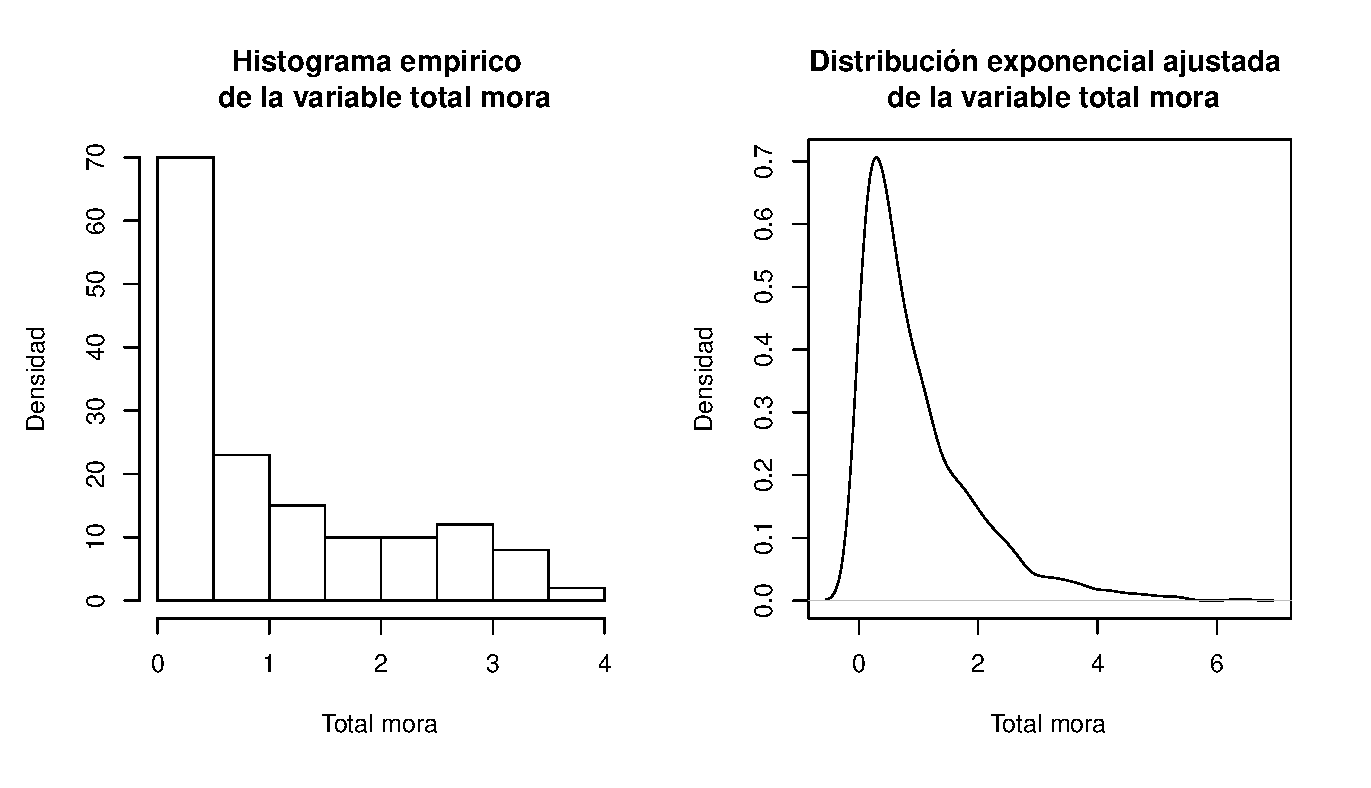
\includegraphics[scale=0.6]{Ajuste_expo_mix.eps}	
		\caption{Ajuste de la distribuci\'{o}n exponencial a la variable \textsl{total mora}}
		\label{Ajuste_expo_mix}
	\end{center}
\end{figure}

Para poder variar el tama\~{n}o de muestra de cada ciudad fue necesario encontrar la distribuci\'{o}n que genera la covariable \textsl{total mora}. En la figura \ref{Ajuste_expo_mix} se muestra como la distribuci\'{o}n exponencial con par\'{a}metro $\lambda=1.075$ describe de forma adecuada el comportamiento de la variable \textsl{total mora} descrita a partir de los datos reales obtenidos en la secci\'{o}n anterior, se eligi\'{o} una distribuci\'{o}n exponencial ya que es una distribuci\'{o}n bastante pertinente para modelar variables de tiempo y en este caso es v\'{a}lido para la definici\'{o}n de la variable \textsl{total mora}.\\

A continuaci\'{o}n se muestran los resultados de la simulaci\'{o}n del modelo de regresi\'{o}n ZOIP-beta mixto, realizada bajo la funci\'{o}n \code{RMM.ZOIP} del paquete \pkg{ZOIP} de \proglang{R}.\\

\begin{table}[!hbt]
{\scriptsize
\begin{center}
\begin{tabular}{|c|c|c|c|c|c|c|c|}\hline
& & \multicolumn{3}{|c|}{Con \textit{pruning}} & \multicolumn{3}{|c|}{Sin \textit{pruning}} \\ \hline
Par\'{a}metro & Valor verdadero de $\beta$'s & $n_i=5$ & $n_i=20$ & $n_i=50$ & $n_i=5$ & $n_i=20$ & $n_i=50$ \\ \hline \hline
\multirow{3}{*}{$\mu$} & $\beta_{10}=-1.13$ & -1.137	&-1.110	&-1.076	&-1.128	&-1.120	&-1.080 \\ 
& $\beta_{11}=0.33$ & 0.321	&0.327	&0.326	&0.331	&0.330	&0.327 \\
& $\lambda_1=0.51$ & 0.879	&0.576	&0.507	&0.882	&0.568	&0.498 \\ \hline
\multirow{3}{*}{$\sigma$} & $\beta_{20}=0.33$ & 0.445	&0.380	&0.336	&0.452	&0.377	&0.345 \\ 
& $\beta_{21}=0.14$ & 0.072	&0.118	&0.132	&0.066	&0.121	&0.133\\
& $\lambda_2=0.4$ & 0.728	&0.450	&0.396	&0.727	&0.456	&0.398\\ \hline
$p_0$& $\beta_{30}=0.23$ &0.220	&0.230	&0.230	&0.220	&0.230	&0.230 \\ \hline
$p_1$& $\beta_{40}=0.07$ &0.060	&0.070	&0.070	&0.060	&0.070	&0.072 \\ \hline
Mediana del tiempo(Seg)& &115.72	&130.85	&140.58	&61.69	&163.36	&218.68 \\ \hline
Mediana del num. iteraciones& &22	&30	&34	&22	&30	&34 \\ \hline
\end{tabular}
\caption{Mediana de los par\'{a}metros estimados en el modelo ZOIP mixto para tres tama\~{n}os de muestra y con la estrategia de con y sin \textit{pruning} y para todos los valores de $Q$.}
\label{T_Sim_mix_ni}
\end{center}
}
\end{table}

En la tabla \ref{T_Sim_mix_ni} se muestran las medianas de los valores estimados para cada uno de los par\'{a}metros del modelo simulado considerando tres tama\~{n}os de muestra $n_i$ y si se utiliz\'{o} \textit{pruning} o no. En dicha tabla se nota como los valores de $\lambda_1$ y $\lambda_2$ asociados a los interceptos aleatorios van convergiendo a su valor verdadero a medida que el tama\~{n}o de muestra va aumentando sin importar si se hizo con o sin \textit{pruning}; adem\'{a}s se nota como las estimaciones de las pendientes $\beta_{11}$ y $\beta_{21}$ va convergiendo a medida que el tama\~{n}o de muestra va creciendo, este par\'{a}metro da un valor muy plausible desde tama\~{n}os de muestra peque\~{n}os, sin importar si se hizo con o sin \textit{pruning}. Este \'{u}ltimo fen\'{o}meno se evidencia tambi\'{e}n con los par\'{a}metros de inflaci\'{o}n $p_0$ y $p_1$ en los que se tiene un valor muy cercano al real desde los tama\~{n}os de muestra peque\~{n}os. En cuesti\'{o}n del tiempo de ejecuci\'{o}n se ve como es reducido en aproximadamente un 50\% cuando se utiliza la metodolog\'{\i}a de la cuadratura de Gauss-Hermite adaptativa con \textit{pruning}, con respecto a no utilizar \textit{pruning}. Sobre el n\'{u}mero de iteraciones se observa como al aumentar el tama\~{n}o de la muestra se requiere una cantidad mayor de iteraciones.\\

\begin{table}[!hbt]
{\scriptsize
\begin{center}
\begin{tabular}{|c|c|c|c|c|c|c|c|}\hline
& & \multicolumn{3}{|c|}{Con \textit{pruning}} & \multicolumn{3}{|c|}{Sin \textit{pruning}} \\ \hline
Par\'{a}metro & Valor verdadero de $\beta$'s & $Q=3$ & $Q=10$ & $Q=20$ & $Q=3$ & $Q=10$ & $Q=20$ \\ \hline \hline
\multirow{3}{*}{$\mu$} & $\beta_{10}=-1.13$ & -1.122	& -1.069	& -1.120	& -1.117	& -1.076	& -1.129 \\ 
& $\beta_{11}=0.33$& 0.323	&0.322	&0.333	&0.334	&0.322	&0.329 \\
& $\lambda_1=0.51$ & 0.632	&0.626	&0.634	&0.629	&0.616	&0.623 \\ \hline
\multirow{3}{*}{$\sigma$} & $\beta_{20}=0.33$ & 0.400	&0.365	&0.366	&0.382	&0.379	&0.373 \\ 
& $\beta_{21}=0.14$ & 0.117	&0.119	&0.120	&0.123	&0.117	&0.121 \\
& $\lambda_2=0.4$& 0.490	&0.487	&0.491	&0.501	&0.482	&0.486 \\ \hline
$p_0$& $\beta_{30}=0.23$ &0.228	&0.228	&0.226	&0.226	&0.226	&0.226 \\ \hline
$p_1$& $\beta_{40}=0.07$ &0.068	&0.070	&0.070	&0.070	&0.068	&0.070 \\ \hline
Mediana del tiempo(Seg)& &75.295	&128.28	&271.825	&74.295	&162.35	&367.545 \\ \hline
Mediana del num. iteraciones& &30	&29	&29	&29	&29	&29 \\ \hline
\end{tabular}
\caption{Mediana de los par\'{a}metros estimados en el modelo ZOIP mixto para tres diferentes n\'{u}meros de puntos de la cuadratura de Gauss-Hermite y con la estrategia de con y sin \textit{pruning} y para todos los tama\~{n}os de muestra.}
\label{T_Sim_mix_ncua}
\end{center}
}
\end{table}

En la tabla \ref{T_Sim_mix_ncua} se muestran las medianas de los valores estimados de cada uno de los par\'{a}metros del modelo simulado considerando tres diferentes n\'{u}meros de puntos de la cuadratura de Gauss-Hermite $Q$ y si se utiliz\'{o} \textit{pruning} o no. En dicha tabla se observa que cuando se utiliza una mayor cantidad de puntos de cuadratura $Q$ se evidencia una peque\~{n}a mejora en la convergencia de los valores reales de los efectos fijos y los componentes de varianza $\lambda_1$ y $\lambda_2$. Con respecto a la utilizaci\'{o}n de \textit{pruning} o no, se observa que las estimaciones de los par\'{a}metros no tienen una diferencia significativa, por lo que es mejor utilizar la cuadratura de Gauss-Hermite adaptativa con \textit{pruning} porque al parecer se obtienen resultados similares, pero con una reducci\'{o}n significativa del tiempo de estimaci\'{o}n de los par\'{a}metros. El n\'{u}mero de iteraciones utilizadas para la estimaci\'{o}n de los par\'{a}metros no se ve influenciado por la cantidad de puntos utilizados en la cuadratura o si se utiliza \textit{pruning} o no.\\

\begin{figure}
	\begin{center}
		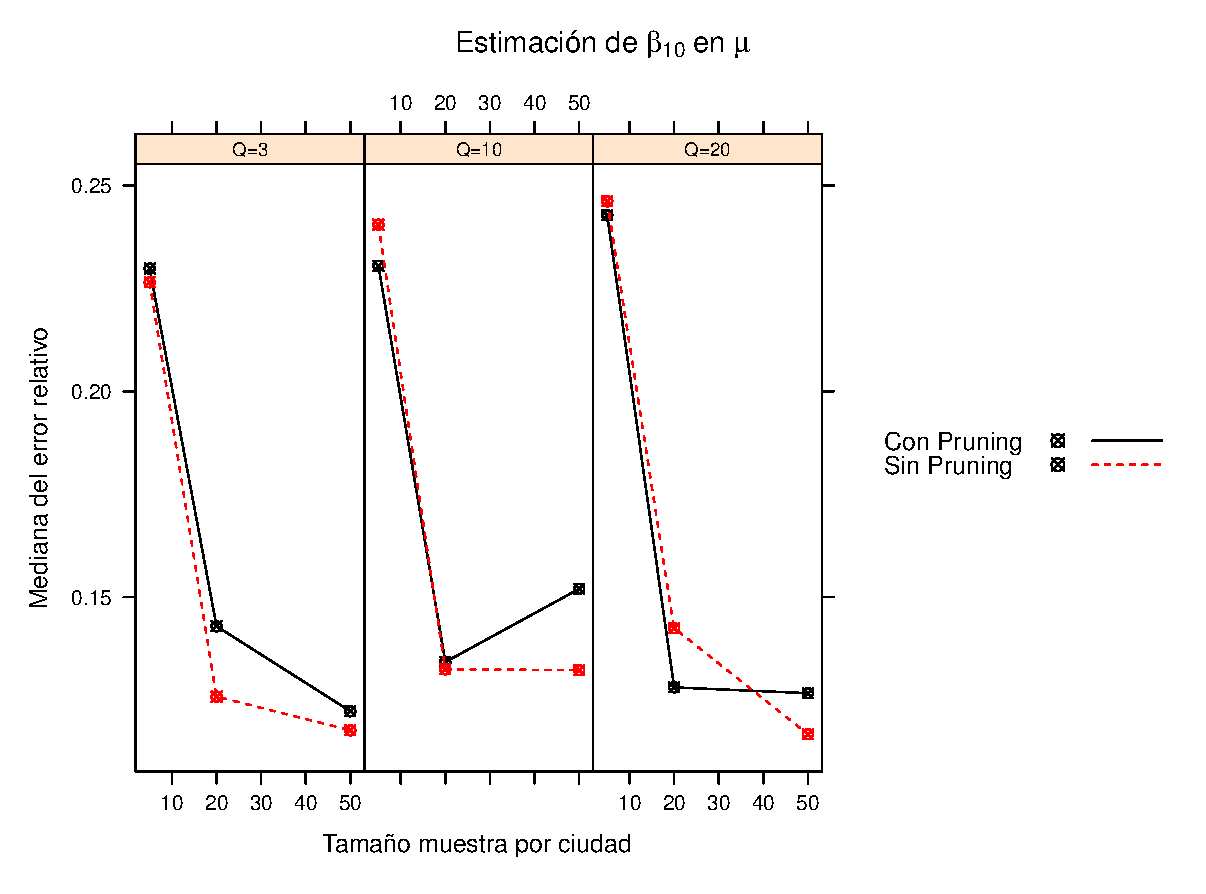
\includegraphics[scale=0.6]{MAPE_beta0_mu.eps}	
		\caption{Mediana del error relativo para la estimaci\'{o}n del par\'{a}metro $\beta_{10}$ asociado a $\mu$, variando el tama\~{n}o de muestra, el n\'{u}mero de puntos de la cuadratura y  la utilizaci\'{o}n de \textit{pruning}.}
		\label{MAPE_bo_mu}
	\end{center}
\end{figure}

La mediana del error relativo de un par\'{a}metro estimado, es \'{u}til para cuantificar en t\'{e}rminos porcentuales el error cometido en la estimaci\'{o}n sin que se vea afectado por algunos valores extremos y es calculado a partir de hallar el error relativo de las 1000 r\'{e}plicas de cada escenario de simulaci\'{o}n para cada par\'{a}metro estimado y calcular la mediana a los mil valores calculados. El error relativo se puede definir como $|(\theta-\hat{\theta})/\theta|$, donde $\theta$ representa cualquier par\'{a}metro del modelo de regresi\'{o}n ZOIP mixto y $\hat{\theta}$ su estimaci\'{o}n.\\

En la figura \ref{MAPE_bo_mu} se muestra la mediana del error relativo sobre el intercepto fijo ($\beta_{10}$) asociado a $\mu$ al variar el tama\~{n}o de muestra $n_i$, el n\'{u}mero de puntos de la cuadratura $Q$ y la utilizaci\'{o}n de \textit{pruning}. En dicha figura se observa que al aumentar el tama\~{n}o de muestra en cada ciudad se obtiene una reducci\'{o}n de la mediana del error relativo de $\beta_{10}$, sin embargo, al aumentar el n\'{u}mero de puntos de la cuadratura se obtienen errores relativos muy parecidos en todos los tama\~{n}os de muestra, por lo que se podr\'{\i}a decir que el aumento del n\'{u}mero de puntos de cuadratura no mejora la estimaci\'{o}n del intercepto fijo sobre el par\'{a}metro $\mu$, por otra parte no se obtiene una diferencia en los errores relativos cuando se utiliza \textit{pruning} y cuando no, aunque, existe un escenario de simulaci\'{o}n cuando el tama\~{n}o de muestra es 50 y $Q=10$ el error relativo de la utilizaci\'{o}n de \textit{pruning} es m\'{a}s grande del que no utiliza.\\



\begin{figure}
	\begin{center}
		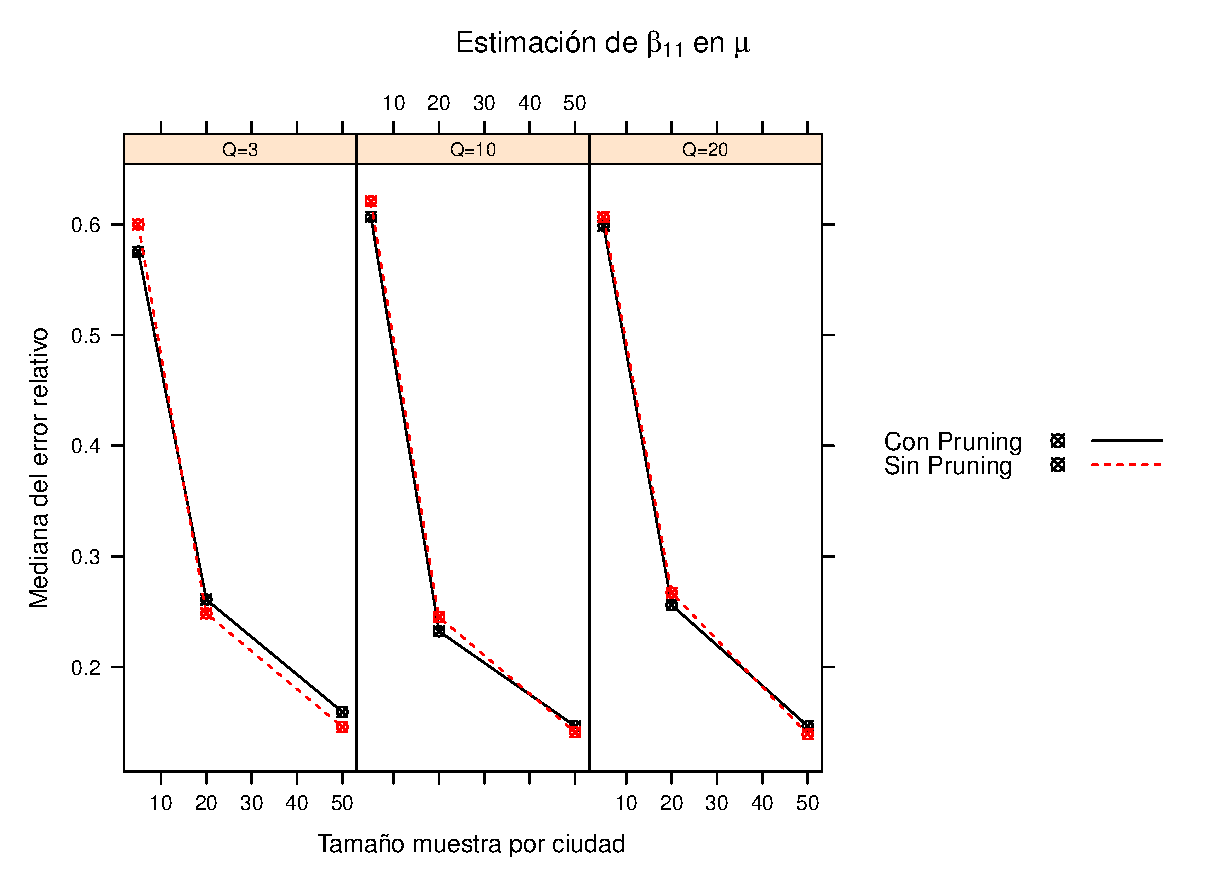
\includegraphics[scale=0.6]{MAPE_beta1_mu.eps}	
		\caption{Mediana del error relativo para la estimaci\'{o}n del par\'{a}metro $\beta_{11}$ asociado a $\mu$, variando el tama\~{n}o de muestra, el n\'{u}mero de puntos de la cuadratura y  la utilizaci\'{o}n de \textit{pruning}.}
		\label{MAPE_beta1_mu}
	\end{center}
\end{figure}

En la figura \ref{MAPE_beta1_mu} se muestra la mediana del error relativo sobre el valor del efecto fijo de la variable \textsl{total mora} sobre $\mu$, a partir de variar el tama\~{n}o de muestra $n_i$, el n\'{u}mero de puntos de la cuadratura $Q$ y si se utiliza \textit{pruning} o no. En dicha figura se muestra como el tama\~{n}o de muestra al ser aumentado obtiene una reducci\'{o}n de la mediana del error relativo, adem\'{a}s al aumentar el n\'{u}mero de puntos de la cuadratura se obtienen errores un poco menores, cuando se aumentan el n\'{u}mero de puntos de la cuadratura, lo que nos permite observar que el aumento del n\'{u}mero de puntos de la cuadratura, no afecta demasiado en la estimaci\'{o}n de este efecto fijo, por otra parte se obtienen errores muy parecidos cuando se utiliza \textit{pruning} y cuando no, por lo que esto no afecta la estimaci\'{o}n del par\'{a}metro.\\


\begin{figure}
	\begin{center}
		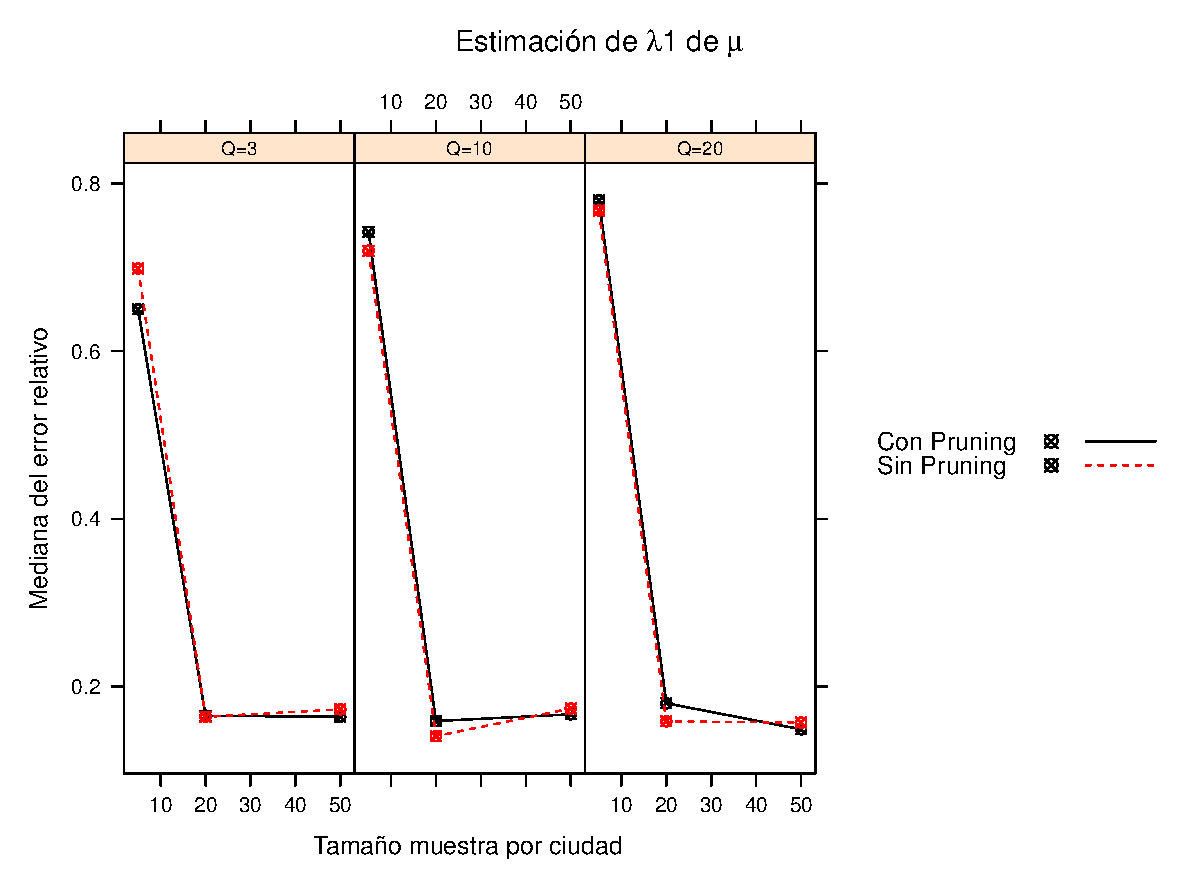
\includegraphics[scale=0.6]{MAPE_lambda1_mu.eps}	
		\caption{Mediana del error relativo para la estimaci\'{o}n del par\'{a}metro $\lambda_1$ desviaci\'{o}n est\'{a}ndar del intercepto aleatorio asociado a la $\mu$, variando el tama\~{n}o de muestra, el n\'{u}mero de puntos de la cuadratura y la utilizaci\'{o}n de \textit{pruning}.}
		\label{MAPE_lambda1_mu}
	\end{center}
\end{figure}

En la figura \ref{MAPE_lambda1_mu} se muestra la mediana del error relativo sobre el valor de la desviaci\'{o}n est\'{a}ndar de la distribuci\'{o}n normal que genera el intercepto aleatorio ($\gamma_1$) del par\'{a}metro de $\mu$, al variar el tama\~{n}o de muestra $n_i$, el n\'{u}mero de puntos de la cuadratura $Q$ y si se utiliza \textit{pruning} o no. En dicha figura se muestra como el tama\~{n}o de muestra al ser aumentado obtiene una reducci\'{o}n de la mediana del error relativo, adem\'{a}s al aumentar el n\'{u}mero de puntos de la cuadratura se obtienen errores menores cuando se aumentan el n\'{u}mero de puntos de la cuadratura, dicha mejora es de alrededor de un 2\% cuando el tama\~{n}o de muestra es m\'{a}s grande $n_i\geq20$ y $Q=20$, este an\'{a}lisis no se ve afectado por el hecho de utilizar \textit{pruning}, por lo que se podr\'{\i}a decir que el aumento del n\'{u}mero de puntos de cuadratura mejora la estimaci\'{o}n del intercepto aleatorio sobre la media cuando el tama\~{n}o de muestra es relativamente grande, por otra parte se obtienen errores relativamente parecidos cuando se utiliza \textit{pruning} y cuando no.\\


\begin{figure}
	\begin{center}
		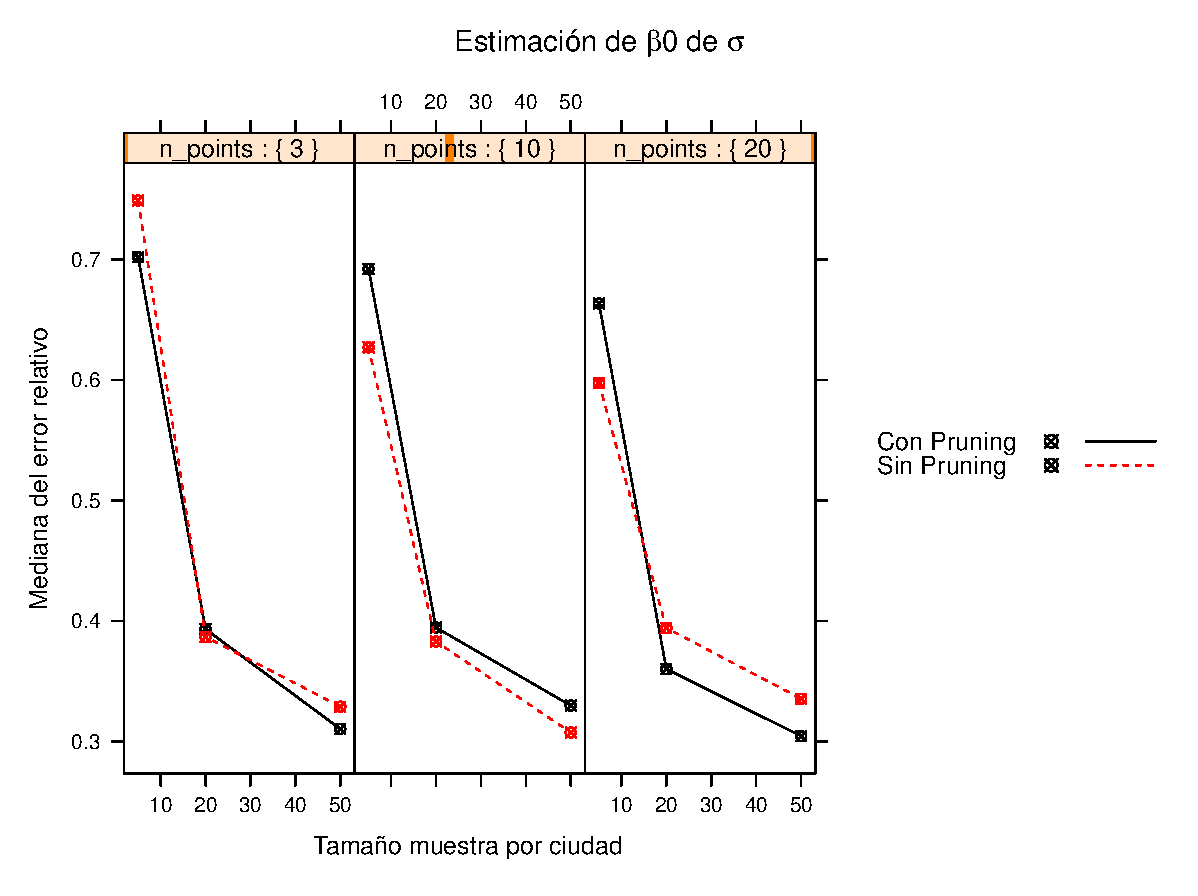
\includegraphics[scale=0.6]{MAPE_beta0_sigma.eps}	
		\caption{Mediana del error relativo para la estimaci\'{o}n del par\'{a}metro $\beta_{20}$ asociado a $\sigma$, variando el tama\~{n}o de muestra, el n\'{u}mero de puntos de la cuadratura y  la utilizaci\'{o}n de \textit{pruning}.}
		\label{MAPE_beta0_sigma}
	\end{center}
\end{figure}

En la figura \ref{MAPE_beta0_sigma} se muestra la mediana del error relativo sobre el intercepto fijo ($\beta_{20}$) del par\'{a}metro de $\sigma$ al variar el tama\~{n}o de muestra $n_i$, el n\'{u}mero de puntos de la cuadratura $Q$ y si se utiliza \textit{pruning} o no. En dicha figura se muestra como cuando se aumenta el tama\~{n}o de muestra en cada ciudad, se obtiene una reducci\'{o}n de la mediana del error relativo, por otra parte al aumentar el n\'{u}mero de puntos de la cuadratura se obtienen errores muy parecidos en todos los tama\~{n}os de muestra, sin embargo, cuando $Q=20$ y se realiza sin la metodolog\'{\i}a \textit{pruning} se nota una reducci\'{o}n en el error, Ahora si observamos las medianas de los errores relativos son relativamente parecidos cuando se utiliza \textit{pruning} y cuando no, sin embargo, se puede rescatar que hay puntos como cuando el tama\~{n}o de muestra es $20$ o $50$ y $Q=20$ el error relativo de la metodolog\'{\i}a sin utilizar \textit{pruning} se ve reducido, mejorando as\'{\i} la estimaci\'{o}n del par\'{a}metro $\beta_{20}$.\\


\begin{figure}
	\begin{center}
		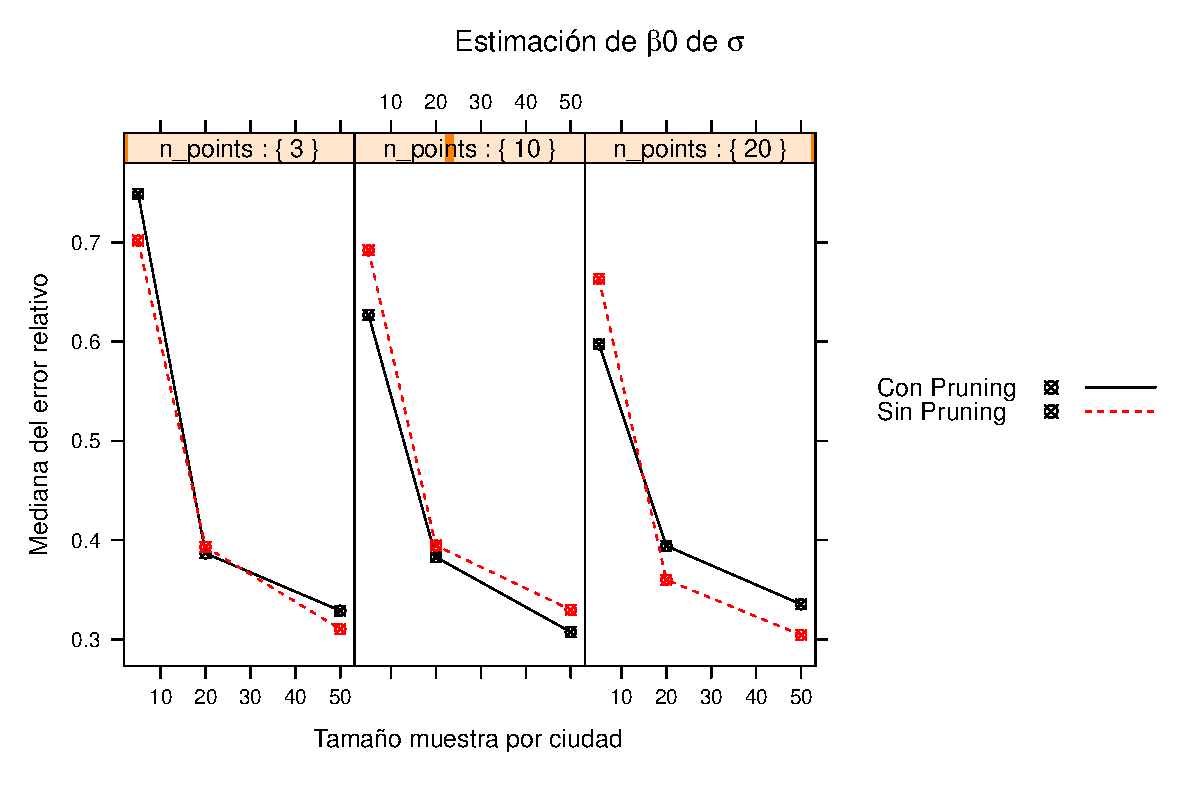
\includegraphics[scale=0.6]{MAPE_beta1_sigma.eps}	
		\caption{Mediana del error relativo para la estimaci\'{o}n del par\'{a}metro $\beta_{21}$ asociado a $\sigma$, variando el tama\~{n}o de muestra, el n\'{u}mero de puntos de la cuadratura y  la utilizaci\'{o}n de \textit{pruning}.}
		\label{MAPE_beta1_sigma}
	\end{center}
\end{figure}

En la figura \ref{MAPE_beta1_sigma} se muestra la mediana del error relativo sobre el valor del efecto fijo de la variable \textsl{total mora} sobre el par\'{a}metro $\sigma$ al variar el tama\~{n}o de muestra $n_i$, el n\'{u}mero de puntos de la cuadratura $Q$ y si se utiliza \textit{pruning} o no. En dicha figura se muestra como el tama\~{n}o de muestra al ser aumentado obtiene una reducci\'{o}n del error relativo, adem\'{a}s al aumentar el n\'{u}mero de puntos de la cuadratura no se obtiene una mejora significativa de la mediana del error relativo, otro aspecto que es importante resaltar es que las estimaciones no se ven afectadas por el hecho de utilizar la metodolog\'{\i}a \textit{pruning}.\\


\begin{figure}
	\begin{center}
		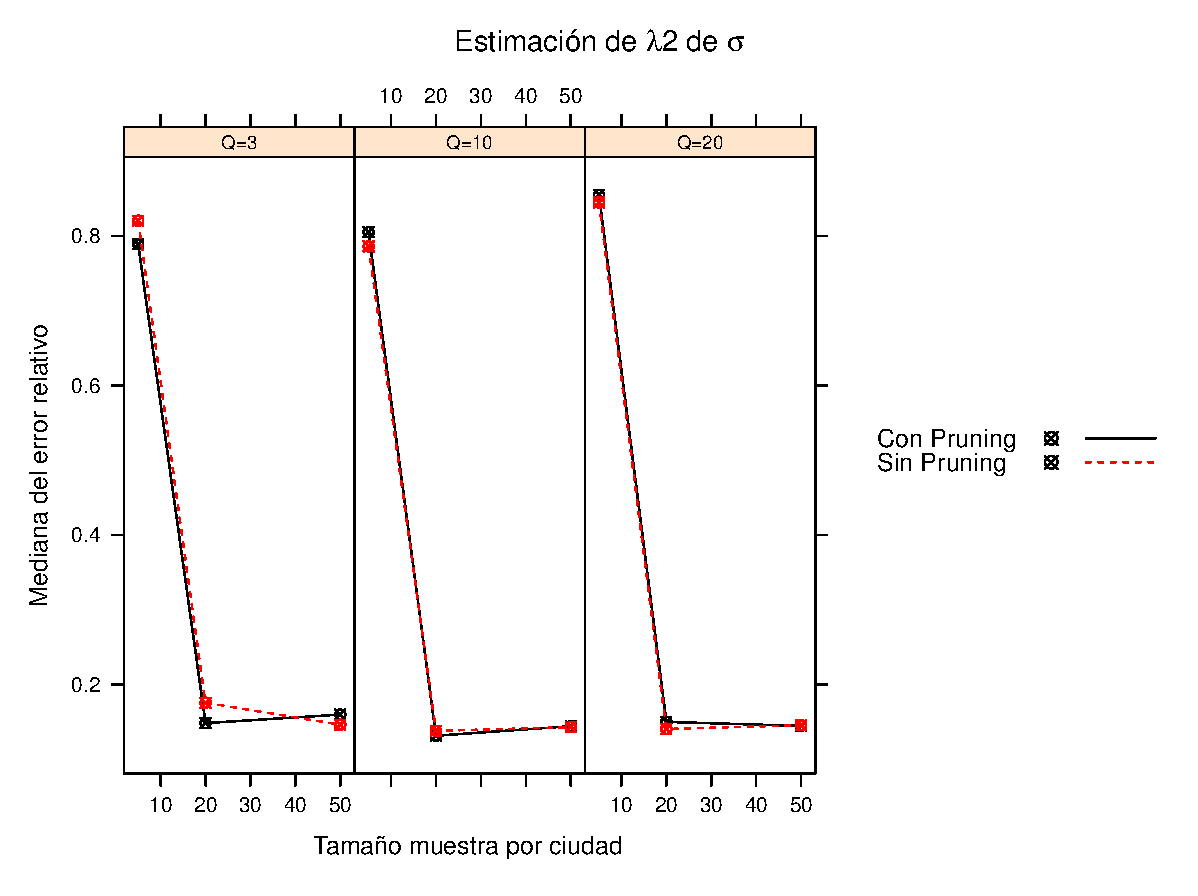
\includegraphics[scale=0.6]{MAPE_lambda2_sigma.eps}	
		\caption{Mediana del error relativo para la estimaci\'{o}n del par\'{a}metro $\lambda_2$ desviaci\'{o}n est\'{a}ndar del intercepto aleatorio asociado a $\sigma$, variando el tama\~{n}o de muestra, el n\'{u}mero de puntos de la cuadratura y la utilizaci\'{o}n de \textit{pruning}.}
		\label{MAPE_lambda2_sigma}
	\end{center}
\end{figure}

En la figura \ref{MAPE_lambda2_sigma} se muestra la mediana del error relativo sobre el valor de la desviaci\'{o}n est\'{a}ndar de la distribuci\'{o}n normal que genera el intercepto aleatorio ($\gamma_2$) del par\'{a}metro de $\sigma$ al variar el tama\~{n}o de muestra $n_i$, el n\'{u}mero de puntos de la cuadratura $Q$ y si se utiliza \textit{pruning} o no. En dicha figura se muestra como el tama\~{n}o de muestra al ser aumentado obtiene una reducci\'{o}n de la mediana del error relativo, adem\'{a}s al aumentar el n\'{u}mero de puntos de la cuadratura se obtienen errores un poco menores, la mejora de alrededor de un 2\% se nota a partir de $Q\geq10$ y cuando los tama\~{n}os de muestra de cada grupo es mayor o igual que 20, adem\'{a}s no se nota una diferencia cuando se utiliza la metodolog\'{\i}a \textit{pruning}, por lo que se podr\'{\i}a decir que el aumento del n\'{u}mero de puntos de cuadratura mejora la estimaci\'{o}n del intercepto aleatorio sobre la dispersi\'{o}n cuando el tama\~{n}o de muestra es relativamente grande, por otra parte se obtienen errores relativamente parecidos cuando se utiliza \textit{pruning} y cuando no, por lo que los valores de las estimaciones no se ven afectadas por la metodolog\'{\i}a \textit{pruning}.\\


\begin{figure}
	\begin{center}
		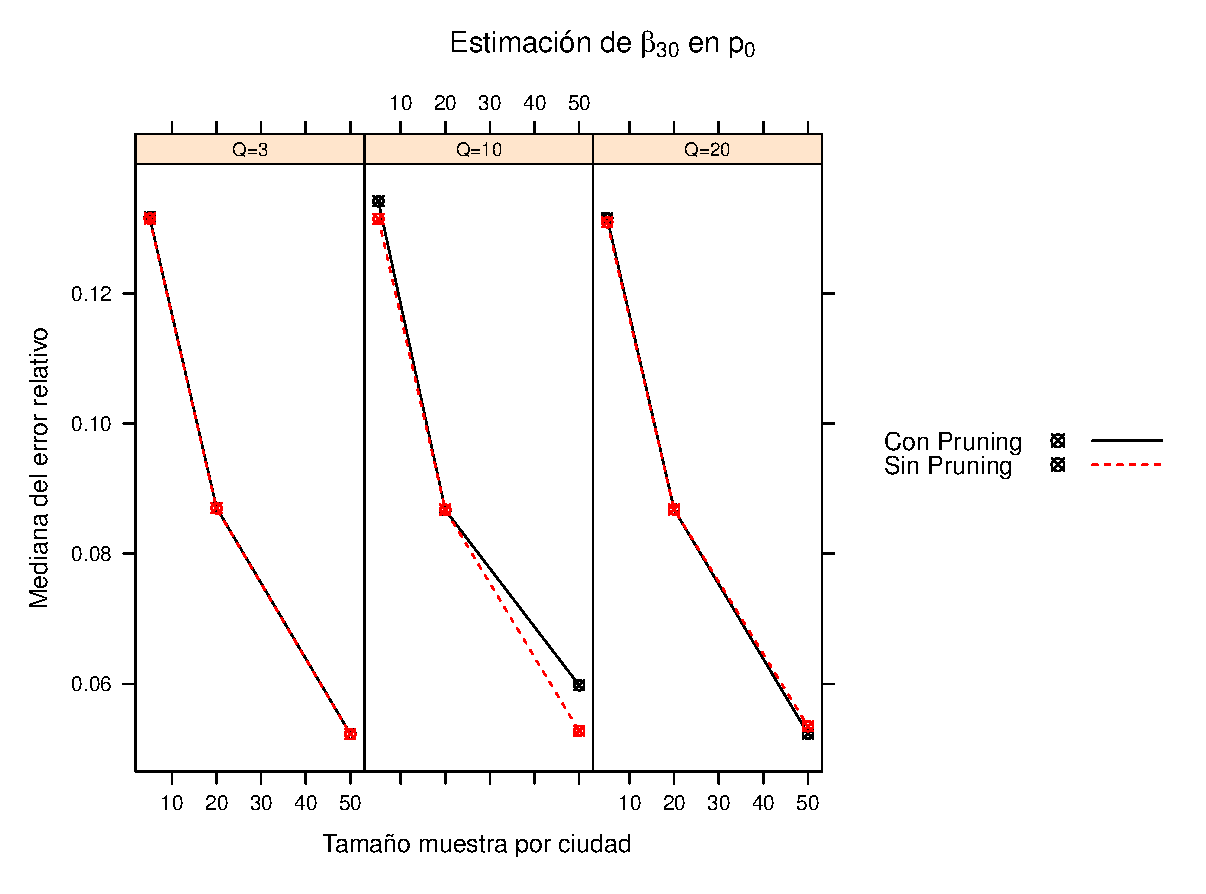
\includegraphics[scale=0.6]{MAPE_beta0_p0.eps}	
		\caption{Mediana del error relativo para la estimaci\'{o}n del par\'{a}metro $\beta_{30}$ asociado al par\'{a}metro de inflaci\'{o}n de ceros, variando el tama\~{n}o de muestra, el n\'{u}mero de puntos de la cuadratura y la utilizaci\'{o}n de \textit{pruning}.}
		\label{MAPE_beta0_p0}
	\end{center}
\end{figure}

En la figura \ref{MAPE_beta0_p0} se muestra la mediana del error relativo sobre el valor de la estimaci\'{o}n del porcentaje de ceros dentro del modelo de regresi\'{o}n ZOIP mixto al variar el tama\~{n}o de muestra $n_i$, el n\'{u}mero de puntos de la cuadratura $Q$ y si se utiliza \textit{pruning} o no. El par\'{a}metro estimado muy bien desde valores de tama\~{n}o de muestra peque\~{n}os, con una mediana del error relativo de alrededor del 13\%, sin embargo, se nota como a medida que el tama\~{n}o de muestra aumenta dicho error decrece r\'{a}pidamente; no se nota una diferencia al variar el n\'{u}mero de puntos de la cuadratura ni sobre la utilizaci\'{o}n de la metodolog\'{\i}a \textit{pruning}.\\

\begin{figure}
	\begin{center}
		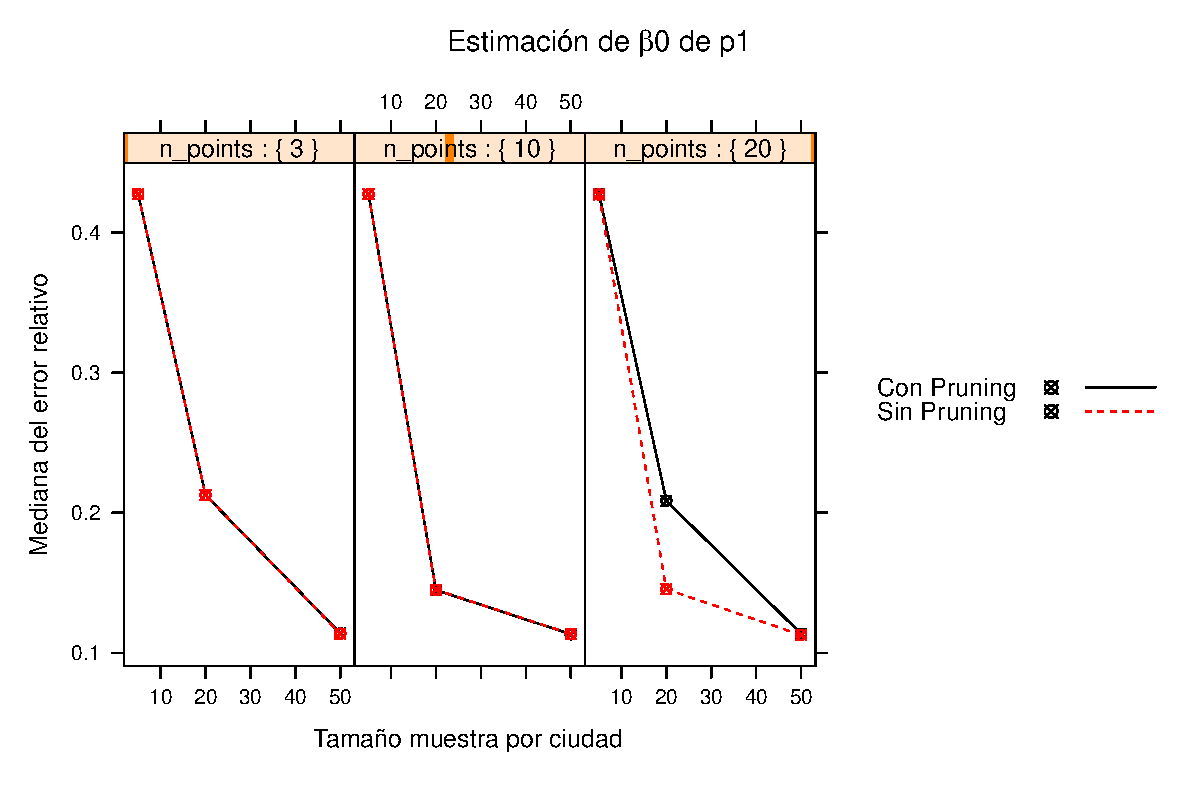
\includegraphics[scale=0.6]{MAPE_beta0_p1.eps}	
		\caption{Mediana del error relativo para la estimaci\'{o}n del par\'{a}metro $\beta_{40}$ asociado al par\'{a}metro de inflaci\'{o}n de unos, variando el tama\~{n}o de muestra, el n\'{u}mero de puntos de la cuadratura y la utilizaci\'{o}n de \textit{pruning}.}
		\label{MAPE_beta0_p1}
	\end{center}
\end{figure}

En la figura \ref{MAPE_beta0_p1} se muestra la mediana del error relativo sobre el valor de la estimaci\'{o}n del porcentaje de unos dentro del modelo de regresi\'{o}n ZOIP mixto al variar el tama\~{n}o de muestra $n_i$, el n\'{u}mero de puntos de la cuadratura $Q$ y si se utiliza \textit{pruning} o no. La estimaci\'{o}n de este par\'{a}metro se ve afectado por el tama\~{n}o de muestra elegido dentro de cada grupo, ya que se nota como al aumentar el tama\~{n}o de muestra la mediana del error relativo decrece r\'{a}pidamente Al aumentar el tama\~{n}o de muestra $n_i$. Adem\'{a}s se puede observar como no hay una diferencia entre la estimaci\'{o}n del par\'{a}metro variando del n\'{u}mero de puntos de la cuadratura ni tampoco sobre la utilizaci\'{o}n de la metodolog\'{\i}a \textit{pruning}, sin embargo cuando $Q=20$ y $n_i=20$, esto no se cumple a cabalidad.\\

\begin{figure}
	\begin{center}
		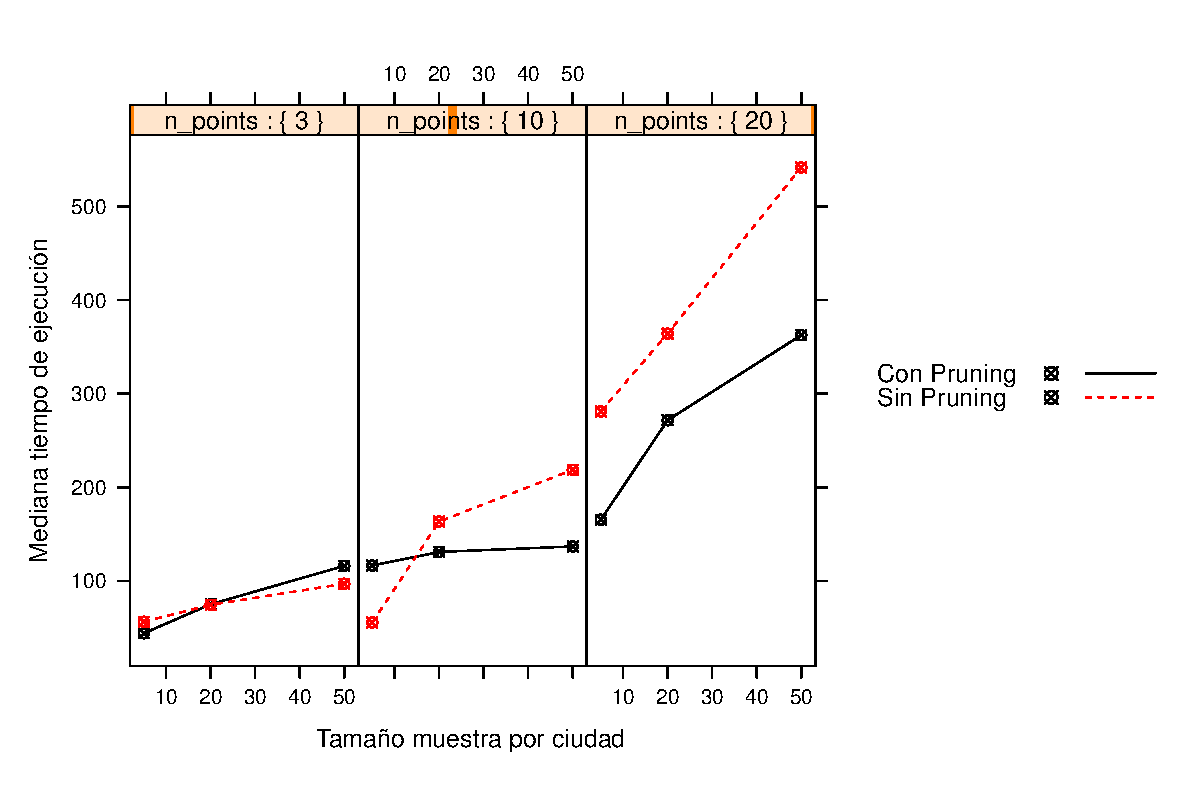
\includegraphics[scale=0.6]{time_mix_ZOIP.eps}	
		\caption{Mediana del tiempo de ejecuci\'{o}n del modelo de regresi\'{o}n ZOIP mixto, bajo la funci\'{o}n de \code{RMM.ZOIP} del paquete \pkg{ZOIP} de \proglang{R}.}
		\label{time_mix_ZOIP}
	\end{center}
\end{figure}

En la figura \ref{time_mix_ZOIP} se muestra la mediana del tiempo de ejecuci\'{o}n para el ajuste del modelo de regresi\'{o}n ZOIP mixto de ejecuci\'{o}n al variar el tama\~{n}o de muestra $n_i$, el n\'{u}mero de puntos de la cuadratura $Q$ y si se utiliza \textit{pruning} o no. Este modelo se ajust\'{o} utilizando la funci\'{o}n \code{RMM.ZOIP} del paquete \pkg{ZOIP}, en dicha figura se nota como a medida que se va aumentando el n\'{u}mero de puntos de la cuadratura y el tama\~{n}o de muestra la diferencia de utilizar la metodolog\'{\i}a \textit{pruning} se hace m\'{a}s favorable ya que se nota una reducci\'{o}n en el tiempo de ejecuci\'{o}n del modelo. Por todo el an\'{a}lisis previo hecho con la estimaci\'{o}n de todos los par\'{a}metros de regresi\'{o}n, en el cual se nota que por lo general sin importar cualquier sea la combinaci\'{o}n entre tama\~{n}o de muestra y el n\'{u}mero de puntos de la cuadratura, la utilizaci\'{o}n de la metodolog\'{\i}a \textit{pruning} no afecta la estimaci\'{o}n de los par\'{a}metros y viendo la figura \ref{time_mix_ZOIP} se ve que es m\'{a}s conveniente utilizar la metodolog\'{\i}a \textit{pruning}, porque esta genera un tiempo de ejecuci\'{o}n menor para ajustar el modelo y sin afectar de la estimaci\'{o}n de los efectos fijos ni de los componentes de varianza del modelo de regresi\'{o}n ZOIP mixto. Adem\'{a}s, se puede concluir que el hecho de aumentar el n\'{u}mero de puntos de la cuadratura s\'{o}lo beneficia a la estimaci\'{o}n de los componentes de varianza mas no de los efectos fijos, en general lo m\'{a}s recomendable para mejorar las estimaciones de todos los par\'{a}metros es aumentar el tama\~{n}o muestra dentro de cada grupo.


%%%%%%%%%%%%%%%%%%%%%%%%%%%%%%%%%%%%%%%%%%%%%%%%%%%%%%%%%%%%%%%%%%%%%%%%%%%%%%%%%%%%%%%%%%%%%%%%%%%%%%%%%%%%%%%%%%%%%%%%%%%%%%%%%%%%%%%%%%%%%%%%%%%%%%%%%%%%%%%%%%

\section{Conclusi\'{o}n}

El modelo de regresi\'{o}n ZOIP con efectos mixtos propuesto en este cap\'{\i}tulo permite modelar los par\'{a}metros de una variable respuesta de datos proporcionales inflados con ceros y/o unos, en funci\'{o}n de un conjunto de covariables. El modelo de regresi\'{o}n ZOIP mixto considera efectos fijos sobre cada uno de los par\'{a}metros de la distribuci\'{o}n ZOIP y permite incluir interceptos aleatorios en los par\'{a}metros de $\mu$ y $\sigma$. La estimaci\'{o}n de los par\'{a}metros del modelo se realiza por m\'{a}xima verosimilitud y con la ayuda de la aproximaci\'{o}n de la cuadratura de Gauss-Hermite adaptativa multidimensional. La estimaci\'{o}n de los par\'{a}metros del modelo puede ser realizada usando la funci\'{o}n \code{RMM.ZOIP} del paquete \pkg{ZOIP}, de una forma amigable para el usuario, en el paquete es posible realizar diferentes tipos de regresi\'{o}n ZOIP mixto, bajo diferentes distribuciones y parametrizaciones, adem\'{a}s de obtener resultados del modelo mediante funciones de metodolog\'{\i}a S3 de \proglang{R}.\\

El estudio de simulaci\'{o}n realizado sobre el modelo de regresi\'{o}n ZOIP mixto, permite sacar variar conclusiones sobre la mejor estimaci\'{o}n de los par\'{a}metros del modelo, una de estas conclusiones es que uno de los factores que mas influyen sobre la estimaci\'{o}n es el tama\~{n}o de muestra de cada uno de los grupos, es decir $n_i$, ya que este factor hace que el error relativo de la estimaci\'{o}n de todos los par\'{a}metros se vea reducido considerablemente cuando se aumenta. Otra conclusi\'{o}n igual de importante es que el hecho de utilizar la metodolog\'{\i}a \textit{pruning} hace que los valores de las estimaciones de los par\'{a}metros del modelo no cambien, pero s\'{\i} que el tiempo de ejecuci\'{o}n se vea reducido en un 50\%. Por ultimo se puede concluir que el efecto del numero de puntos de la cuadratura de Gauss-Hermite no influye demasiado en la estimaci\'{o}n de los par\'{a}metros de efectos fijos, aunque s\'{\i} afecta el aumento de este factor la estimaci\'{o}n de los componentes de varianza de los interceptos aleatorios, un numero prudente de puntos es entre cinco y quince, ya que el aumento considerado de este factor no influye en la mejor\'{\i}a de la estimaci\'{o}n de los par\'{a}metros, pero si en el aumento del tiempo de ejecuci\'{o}n.   
\chapter{Conclusiones y recomendaciones}\label{cap5}
\section{Conclusiones}

En este trabajo se propone una nueva clase de distribuciones y modelos de regresi\'{o}n para efectos fijos y mixtos para datos proporcionales inflados con ceros y/o unos, en la distribuci\'{o}n propuesta y los dos modelos de regresi\'{o}n, se integran tres diferentes parametrizaciones de la distribuci\'{o}n beta, adem\'{a}s a manera de distribuci\'{o}n alternativa de la beta se integra la distribuci\'{o}n simplex, estos modelos y distribuciones son muy flexibles, ya que en una sola distribuci\'{o}n o modelo de regresi\'{o}n se obtienen diferentes opciones de modelado.\\

La distribuci\'{o}n propuesta y en la que se basan todos los modelos de regresi\'{o}n, es la distribuci\'{o}n ZOIP, esta distribuci\'{o}n permite obtener diferentes distribuciones para datos proporciones inflados con ceros y/o unos, dicha distribuci\'{o}n permite ajustarse a datos que se encuentran inflados solo con ceros o solo con unos, incluso a datos proporcionales tradicionales, es decir, sin inflaciones. El modelo de regresi\'{o}n ZOIP es propuesto en este trabajo como el ajuste de un modelo de regresi\'{o}n con efectos fijos en los cuatro par\'{a}metros de distribuci\'{o}n ZOIP y es ajustado v\'{\i}a m\'{a}xima verosimilitud. Por \'{u}ltimo, se propone el modelo de regresi\'{o}n ZOIP mixto, el cual permite ajustar un modelo de regresi\'{o}n con efectos fijos en todos los par\'{a}metros de la distribuci\'{o}n ZOIP y tener en cuenta interceptos aleatorios normales en el par\'{a}metro de la media y la varianza, la estimaci\'{o}n de los par\'{a}metros fue realizada v\'{\i}a m\'{a}xima verosimilitud y mediante la aproximaci\'{o}n de la funci\'{o}n de verosimilitud, por medio de las diferentes alternativas de la cuadratura de Gauss-Hermite adaptativa multidimensional.\\
 
Fue propuesto un paquete de \proglang{R} llamado \pkg{ZOIP}, que permite obtener valores de la funci\'{o}n de densidad de probabilidad, funciones de distribuci\'{o}n acumulada y funci\'{o}n cuantil de la distribuci\'{o}n ZOIP, adem\'{a}s de generaci\'{o}n de valores aleatorios de dicha distribuci\'{o}n. Por otra parte, el paquete permite ajustar distribuciones ZOIP o modelos de regresi\'{o}n ZOIP, mediante algoritmos de optimizaci\'{o}n, como \code{nlimnb} o \code{optim}. Tambi\'{e}n, es posible ajustar los modelos de regresi\'{o}n ZOIP mixto, v\'{\i}a m\'{a}xima verosimilitud y la cuadratura de Gauss-Hermite adaptativa. El paquete \pkg{ZOIP}, tambi\'{e}n incluye en el ajuste de sus modelos algunas funciones de m\'{e}todo S3.\\

Se realizaron estudios de simulaci\'{o}n que permitieron ver la convergencia de los par\'{a}metros en el ajuste de la distribuci\'{o}n ZOIP, el modelo de regresi\'{o}n ZOIP y el modelo de regresi\'{o}n ZOIP mixto, adem\'{a}s esto permiti\'{o} concluir con que alternativas se encuentran las mejores estimaciones de los par\'{a}metros regresores de los modelos. En el modelo de regresi\'{o}n ZOIP mixto se encontr\'{o} que el hecho de utilizar la metodolog\'{\i}a \textit{pruning} ayuda a reducir los tiempos de ajuste del modelo en un 50\% cuando se utilizan grandes tama\~{n}os de muestra y el n\'{u}mero de puntos de la cuadratura de Gauss-Hermite es grande, adem\'{a}s se evidencio que el aumento del n\'{u}mero de puntos de la cuadratura afecta de manera positiva y en mayor proporci\'{o}n a los par\'{a}metros asociados a los interceptos aleatorios de los par\'{a}metros de la media y la varianza. Por \'{u}ltimo, se encontr\'{o} en todos los modelos que el aumento del tama\~{n}o de muestra es el mayor factor que hace que la estimaci\'{o}n de los par\'{a}metros regresores mejoren, considerablemente.\\

Por ultimo se realizaron aplicaciones a datos reales, para el ajuste de, distribuciones ZOIP, modelos de regresi\'{o}n ZOIP y modelos de regresi\'{o}n ZOIP mixtos sobre el porcentaje de utilizaci\'{o}n de una tarjeta de cr\'{e}dito asociada a una entidad financiera, en dicha aplicaci\'{o}n se evidencio que el ajuste de los modelos fueron satisfactorios y  fue posible encontrar diferentes factores que afectan al porcentaje de utilizaci\'{o}n de las tarjetas de cr\'{e}dito, lo que permitir\'{\i}a sacar conclusiones muy importantes para estrategias de mercadeo y fidelizaci\'{o}n de los clientes de la entidad financiera.


\section{Recomendaciones}

Como posibles trabajos futuros y recomendaciones se propone:

\begin{itemize}
	\item Extender la distribuci\'{o}n ZOIP a otras distribuciones para datos proporcionales no tomadas en cuenta en este trabajo, tales como la distribuci\'{o}n beta-rectangular y la distribuci\'{o}n LogitSep.
	\item Realizar un estudio de an\'{a}lisis de residuales para los par\'{a}metros estimados de los modelos de regresi\'{o}n ZOIP fijos y mixtos.
	\item Incluir un an\'{a}lisis de selecci\'{o}n de modelos en los modelos de regresi\'{o}n ZOIP fijos y mixtos.
	\item Incluir interceptos aleatorios en los par\'{a}metros asociados a la inflaci\'{o}n de la distribuci\'{o}n ZOIP, en el modelo de regresi\'{o}n ZOIP mixto, propuesto en este trabajo.
\item Incluir pendientes aleatorias en los diferentes par\'{a}metros de la regresi\'{o}n ZOIP.
	\item Extender los interceptos alea tiros en los par\'{a}metros de la media y la dispersi\'{o}n, a interceptos aleatorios no normales, o normales correlacionados.
	\item Incluir m\'{a}s funciones de m\'{e}todo S3 en el paquete \pkg{ZOIP}, tales como \code{plot}, \code{predict} \code{AIC}, \code{BIC}, entre otras.
	\item Realizar una comparaci\'{o}n entre la estimaci\'{o}n de los par\'{a}metros del modelo de regresi\'{o}n ZOIP mixto, por metodolog\'{\i}as bayesianas y utilizando m\'{a}xima verosimilitud y la cuadratura de Gauss-Hermite adaptativa.
		\item Mejorar la eficiencia de los algoritmos implementados en el paquete \pkg{ZOIP}, mediante la integraci\'{o}n del paquete \pkg{ZOIP} por las metodolog\'{\i}as implementadas en el paquete \pkg{RCPP}.
	\item Estudiar e implementar otras metodolog\'{\i}as de estimaci\'{o}n de los par\'{a}metros, nunca exploradas sobre los modelos de regresi\'{o}n mixtos para datos proporcionales inflados con ceros y/o con unos, tales como la metodolog\'{\i}a bayesiana INLA o los algoritmos propuestos por \cite{Ogden1}, sobre m\'{e}todos de reducci\'{o}n secuencial. 
	\item Evaluar m\'{a}s la simulaci\'{o}n del modelo de regresi\'{o}n ZOIP mixto propuesto, para las dem\'{a}s parametrizaciones de la distribuci\'{o}n ZOIP-beta y la distribuci\'{o}n ZOIP-simplex.
	\item Optimizar los algoritmos propuestos en el paquete \pkg{ZOIP}, para que el tiempo de estimaci\'{o}n los par\'{a}metros sean m\'{a}s cortos.
	\item Estudiar t\'{o}picos de los datos proporcionales inflados para datos proporcionales inflados con ceros y/o unos, como cuando m\'{a}s del 50\% de la muestra se encuentra inflada por ceros o por unos. se podr\'{\i}a evaluar la eficacia y convergencia de las funciones implementadas, en el paquete \pkg{ZOIP} mediante estudios de simulaci\'{o}n.
	\item Realizar mejoras continuas del paquete \pkg{ZOIP}, a medida que se vayan adquiriendo retroalimentaciones de los usuarios que utilizan el paquete.
	\item Extender los estudios de simulaci\'{o}n del modelo de regresi\'{o}n ZOIP mixto, cuando se tienen muestras no balanceadas.

\end{itemize}

\nocite{Seoane1}
\nocite{Lindstrom1}
\nocite{Evans1}
\nocite{kieschnick1}
\nocite{Cook1}
\nocite{Houston1}
\nocite{Venezuela1}
\nocite{Git1}

\chapter{Conclusiones y recomendaciones}
\section{Conclusiones}
Las conclusiones constituyen un cap\'{\i}tulo independiente y presentan, en forma l\'{o}gica, los resultados de la tesis  o trabajo de investigaci\'{o}n. Las conclusiones deben ser la respuesta a los objetivos o prop\'{o}sitos planteados. Se deben titular con la palabra conclusiones en el mismo formato de los t\'{\i}tulos de los cap\'{\i}tulos anteriores (T\'{\i}tulos primer nivel), precedida por el numeral correspondiente (seg\'{u}n la presente plantilla).\\

\section{Recomendaciones}
Se presentan como una serie de aspectos que se podr\'{\i}an realizar en un futuro para emprender investigaciones similares o fortalecer la investigaci\'{o}n realizada. Deben contemplar las perspectivas de la investigaci\'{o}n, las cuales son sugerencias, proyecciones o alternativas que se presentan para modificar, cambiar o incidir sobre una situaci\'{o}n espec\'{\i}fica o una problem\'{a}tica encontrada. Pueden presentarse como un texto con caracter\'{\i}sticas argumentativas, resultado de una reflexi\'{o}n acerca de la tesis o trabajo de investigaci\'{o}n.\\
\begin{appendix}
\chapter{Anexo: Nombrar el anexo A de acuerdo con su contenido}\label{AnexoA}
Los Anexos son documentos o elementos que complementan el cuerpo de la tesis o trabajo de investigaci\'{o}n y que se relacionan, directa o indirectamente, con la investigaci\'{o}n, tales como acetatos, cd, normas, etc.\\

\chapter{Anexo: Nombrar el anexo B de acuerdo con su contenido}
A final del documento es opcional incluir \'{\i}ndices o glosarios. \'{E}stos son listas detalladas y especializadas de los t\'{e}rminos, nombres, autores, temas, etc., que aparecen en el mismo. Sirven para facilitar su localizaci\'{o}n en el texto. Los \'{\i}ndices pueden ser alfab\'{e}ticos, cronol\'{o}gicos, num\'{e}ricos, anal\'{\i}ticos, entre otros. Luego de cada palabra, t\'{e}rmino, etc., se pone coma y el n\'{u}mero de la p\'{a}gina donde aparece esta informaci\'{o}n.\\

\chapter{Anexo: Nombrar el anexo C de acuerdo con su contenido}
MANEJO DE LA BIBLIOGRAF\'{I}A: la bibliograf\'{\i}a es la relaci\'{o}n de las fuentes documentales consultadas por el investigador para sustentar sus trabajos. Su inclusi\'{o}n es obligatoria en todo trabajo de investigaci\'{o}n. Cada referencia bibliogr\'{a}fica se inicia contra el margen izquierdo.\\

La NTC 5613 establece los requisitos para la presentaci\'{o}n de referencias bibliogr\'{a}ficas citas y notas de pie de p\'{a}gina. Sin embargo, se tiene la libertad de usar cualquier norma bibliogr\'{a}fica de acuerdo con lo acostumbrado por cada disciplina del conocimiento. En esta medida es necesario que la norma seleccionada se aplique con rigurosidad.\\

Es necesario tener en cuenta que la norma ISO 690:1987 (en Espa\~{n}a, UNE 50-104-94) es el marco internacional que da las pautas m\'{\i}nimas para las citas bibliogr\'{a}ficas de documentos impresos y publicados. A continuaci\'{o}n se lista algunas instituciones que brindan par\'{a}metros para el manejo de las referencias bibliogr\'{a}ficas:\\

\begin{center}
\centering%
\begin{tabular}{|p {7.5 cm}|p {7.5 cm}|}\hline
\arr{Instituci\'{o}n}&Disciplina de aplicaci\'{o}n\\\hline%
Modern Language Association (MLA)&Literatura, artes y humanidades\\\hline%
American Psychological Association (APA)&Ambito de la salud (psicolog\'{\i}a, medicina) y en general en todas las ciencias sociales\\\hline
Universidad de Chicago/Turabian &Periodismo, historia y humanidades.\\\hline
AMA (Asociaci\'{o}n M\'{e}dica de los Estados Unidos)&Ambito de la salud (psicolog\'{\i}a, medicina)\\\hline
Vancouver &Todas las disciplinas\\\hline
Council of Science Editors (CSE)&En la actualidad abarca diversas ciencias\\\hline
National Library of Medicine (NLM) (Biblioteca Nacional de Medicina)&En el \'{a}mbito m\'{e}dico y, por extensi\'{o}n, en ciencias.\\\hline
Harvard System of Referencing Guide &Todas las disciplinas\\\hline
JabRef y KBibTeX &Todas las disciplinas\\\hline
\end{tabular}
\end{center}

Para incluir las referencias dentro del texto y realizar lista de la bibliograf\'{\i}a en la respectiva secci\'{o}n, puede utilizar las herramientas que Latex suministra o, revisar el instructivo desarrollado por el Sistema de Bibliotecas de la Universidad Nacional de Colombia\footnote{Ver: www.sinab.unal.edu.co}, disponible en la secci\'{o}n "Servicios", opci\'{o}n "Tr\'{a}mites" y enlace "Entrega de tesis".

\end{appendix}
\addcontentsline{toc}{chapter}{\numberline{}Bibliograf\'{\i}a}
\bibliographystyle{plainnat}
\bibliography{BibliMSc}
\end{document}